% \iffalse meta-comment
% 
% 
% Copyright (C) 2009,2010,2011,2012 by Martin Wilhelm Leidig 
% <mwl@moss.in-berlin.de>
% Copyright (C) 2015,2016 by Enterprise Modelling and Information 
% Systems Architectures - An International Journal (EMISA)
% --------------------------------------------------------------------
%
% This work may be distributed and/or modified under the
% conditions of the LaTeX Project Public License (LPPL), either
% version 1.3c of this license or (at your option) any later
% version.  The latest version of this license is in the file:
%
% http://www.latex-project.org/lppl.txt
%
% This work is "maintained" (as per LPPL maintenance status) by
% Stefan Strecker <stefan.strecker@fernuni-hagen.de> and 
% Martin Sievers <martin.sievers@schoenerpublizieren.de>.
%
% This work consists of all files listed in manifest.txt.
%
% \fi
% 
% \CheckSum{0}
% \CharacterTable
%  {Upper-case    \A\B\C\D\E\F\G\H\I\J\K\L\M\N\O\P\Q\R\S\T\U\V\W\X\Y\Z
%   Lower-case    \a\b\c\d\e\f\g\h\i\j\k\l\m\n\o\p\q\r\s\t\u\v\w\x\y\z
%   Digits        \0\1\2\3\4\5\6\7\8\9
%   Exclamation   \!     Double quote  \"     Hash (number) \#
%   Dollar        \$     Percent       \%     Ampersand     \&
%   Acute accent  \'     Left paren    \(     Right paren   \)
%   Asterisk      \*     Plus          \+     Comma         \,
%   Minus         \-     Point         \.     Solidus       \/
%   Colon         \:     Semicolon     \;     Less than     \<
%   Equals        \=     Greater than  \>     Question mark \?
%   Commercial at \@     Left bracket  \[     Backslash     \\
%   Right bracket \]     Circumflex    \^     Underscore    \_
%   Grave accent  \`     Left brace    \{     Vertical bar  \|
%   Right brace   \}     Tilde         \~}
%
% \iffalse
%<*driver>
\ProvidesFile{emisa.dtx}
%</driver>
%<class>\NeedsTeXFormat{LaTeX2e}[1999/12/01]
%<class>\ProvidesClass{emisa}%
%<*class>
[2016/01/12 2.0BETA LaTeX class EMISA]
%</class>
%
%<*driver>
\begingroup 
%</driver>
%<*batchfile>
\input docstrip.tex
\keepsilent
\askforoverwritefalse
% \askforoverwritetrue
\askonceonly 
%<batchfile>\showprogress
%<batchfile>\askforoverwritetrue
% \usedir{tex/latex/\jobname}
%%% 
% this is for biblatex files:
\declarepreamble\biblatexpre

This file is part of the \jobname.cls interface to the biblatex package.
See there for more information.
------------------------------------------------------------------------

\endpreamble
%%% 
% this is for template files:
\declarepreamble\templatepre

This is a template for a document to be used with \jobname.cls.  
Just copy (not move) this file to your work space, and rename and use
it as you see fit.
------------------------------------------------------------------------

\endpreamble
%%% 
% this is for the class itself:
\declarepreamble\classpre

If you absolutely have to change \outFileName, please
do so in \jobname.dtx (after altering the name, of course!).

Copyright (C) 2009,2010,2011,2012 by Martin Wilhelm Leidig 
<mwl@moss.in-berlin.de>
Copyright (C) 2015,2016 by Enterprise Modelling and Information 
Systems Architectures - An International Journal (EMISA)
------------------------------------------------------------------------

This work may be distributed and/or modified under the
conditions of the LaTeX Project Public License (LPPL), either
version 1.3c of this license or (at your option) any later
version.  The latest version of this license is in the file:

http://www.latex-project.org/lppl.txt

This work is "maintained" (as per LPPL maintenance status) by
Stefan Strecker <stefan.strecker@fernuni-hagen.de> and 
Martin Sievers <martin.sievers@schoenerpublizieren.de>.

This work consists of all files listed in manifest.txt.
------------------------------------------------------------------------

\endpreamble
\AddGenerationDate
\generate{%
  \usepreamble\classpre
  \file{\jobname.cls}{\from{\jobname.dtx}{class}}
  \file{\jobname.ins}{\from{\jobname.dtx}{batchfile}}
  \usepreamble\biblatexpre
  \file{\jobname.bbx}{\from{\jobname.dtx}{biblatex,bbx}}
  \file{\jobname.cbx}{\from{\jobname.dtx}{biblatex,cbx}}
  \usepreamble\templatepre
  \file{\jobname-author-template.tex}{\from{\jobname.dtx}{template,article}}
}

\obeyspaces
\Msg{**********************************************************************}
\Msg{*}
\Msg{* To finish the installation you have to move the following}
\Msg{* file(s) into a directory searched by TeX.  In the following,}
\Msg{* TEXMF stands for any of the texmf trees in your system,}
\Msg{* probably the system-local or the user-local one.}
\Msg{*}
\Msg{* The class itself and the system-local configuration file}
\Msg{* is placed best in TEXMF/tex/latex/emisa:}
\Msg{*     \jobname.cls}
\Msg{*}
\Msg{* In most cases simply keeping those all together in the same}
\Msg{* directory might be the best solution.}
\Msg{*}
\Msg{* To produce the source documentation run the file \jobname.dtx}
\Msg{* through LaTeX; at least twice to get the cross references right.}
\Msg{* If you want an index after that, you need to run}
\Msg{*}
\Msg{*     makeindex -s gind.ist \jobname.idx}
\Msg{*}
\Msg{* and/or for a change history, use MakeIndex like this:}
\Msg{*}
\Msg{*     makeindex -s gglo.ist -o \jobname.gls \jobname.glo}
\Msg{*}
\Msg{* Then run LaTeX another time.}
\Msg{* Happy TeXing!}
\Msg{*}
\Msg{**********************************************************************}
%<batchfile>\endbatchfile
%</batchfile>
%<*driver>
\endgroup
%</driver>
%<*driver>
\documentclass[a4paper]{ltxdoc}
\usepackage[olddocinclude]{xdoc2}
\usepackage[british]{babel}
\usepackage[utf8]{inputenc}
\usepackage[T1]{fontenc}
\usepackage{newtxtext}
\usepackage[strict]{csquotes}
\usepackage{amssymb}
\usepackage{xspace}
\usepackage{fancyvrb}
\usepackage[lmargin=4.5cm,rmargin=2cm,bottom=4cm,top=2cm]{geometry}
\usepackage{array,booktabs,tabularx}
\usepackage{listings,lstautogobble}
\lstset{%
  extendedchars,
  language=[LaTeX]TeX,
  basicstyle=\MacroFont,
  commentstyle={\color{black!50}\bfseries},
  keywordstyle={},
  breaklines,
  emptylines=1,
  gobble=2
  }
\lstnewenvironment{examplecode}
{}
{}  
\usepackage[onehalfspacing]{setspace}
\usepackage[dvipsnames]{xcolor}
%\usepackage{hologo}
\usepackage{graphicx}
\usepackage[alwaysadjust,flushright]{paralist}
\setdefaultleftmargin{1.2em}{1.2em}{1.2em}{1.2em}{1.2em}{1.2em}%
\setdefaultenum{(1)}{}{}{}% 
\setdefaultitem
  {\textcolor{codelinenocolor}{$\vartriangleright$}}%
  {\textcolor{codelinenocolor}{$\circ$}}%
  {\textcolor{codelinenocolor}{\textendash}}%
  {\textcolor{codelinenocolor}{\textperiodcentered}}% 
\let\itemize\compactitem
\let\enditemize\endcompactitem
\let\enumerate\compactenum
\let\endenumerate\endcompactenum
\let\description\compactdesc
\let\enddescription\endcompactdesc
\colorlet{linkcolor}{red!80!blue}
\colorlet{anchorcolor}{black}
\colorlet{citecolor}{green!67!blue}
\colorlet{filecolor}{linkcolor}
\colorlet{urlcolor}{blue!80!black}
\usepackage[%
   pdftitle={},
   pdfauthor={},
   breaklinks,
   pagebackref,
   backref,
   hyperindex,
   linktocpage,
   bookmarksopen,
   bookmarksnumbered,
   colorlinks,
   linkcolor=linkcolor,
   anchorcolor=anchorcolor,
   citecolor=citecolor,
   filecolor=filecolor,
   urlcolor=urlcolor]{hyperref}
%
\providecommand*\pkg[1]{\textsf{#1}}
\makeatletter
\newcommand*\DescribeOption{%
   \leavevmode%
   \@bsphack%
   \begingroup%
    \MakePrivateLetters%
    \Describe@Option%
}%
\newcommand*\Describe@Option[1]{%
   \endgroup%
   \marginpar{%
      \raggedleft%
      \PrintDescribeEnv{#1}%
   }%
   \SpecialOptionIndex{#1}%
   \@esphack%
   \ignorespaces%
}%
\newcommand*\SpecialOptionIndex[1]{%
   \@bsphack%
   \index{%
      #1\actualchar{\protect\ttfamily#1} (option)\encapchar usage%
   }%
   \index{%
      options:\levelchar#1\actualchar{\protect\ttfamily#1}%
      \encapchar usage%
   }%
   \@esphack%
}%
%
\newcommand{\DTXname}{\jobname}
\newcommand{\DTXclassname}{\texorpdfstring{\cls{\MakeUppercase{\DTXname}}\xspace}{\DTXname}}
% 
\hfuzz200pt
% 
\parskip = 0.5\baselineskip plus  0.5\baselineskip
\setlength{\parindent}{0em}
% 
\renewcommand*\textfraction{0.01}%
\renewcommand*\topfraction{0.9}%
\let\bottomfraction\topfraction%
% 
\makeatletter
% \renewcommand*\l@section{\@dottedtocline{1}{0mm}{2.5em}}
\renewcommand*\l@subsection{\@dottedtocline{2}{0mm}{4.5em}}
\renewcommand*\l@subsubsection{\@dottedtocline{3}{0em}{4.5em}}
\renewcommand*\l@paragraph{\@dottedtocline{4}{0em}{6.5em}}
\renewcommand*\l@subparagraph{\@dottedtocline{5}{0em}{6.5em}}
\renewcommand*\l@figure{\@dottedtocline{1}{0mm}{2.5em}}
% \let\l@figure\l@subsection
\let\l@table\l@figure
\makeatother
%%%\numberwithin{figure}{section}
%%%\numberwithin{table}{section}
% 
\DeclareRobustCommand{\opt}[1]{{\fontfamily\ttdefault\upshape #1}}
\DeclareRobustCommand{\arg}[1]{{\fontfamily\ttdefault\upshape #1}}
\DeclareRobustCommand{\env}[1]{{\fontfamily\ttdefault\upshape #1}}
\DeclareRobustCommand{\pkg}[1]{{\fontfamily\sfdefault\upshape #1}}
\DeclareRobustCommand{\cls}[1]{{\normalfont\fontfamily\sfdefault\upshape #1}}
\DeclareRobustCommand{\file}[1]{{\fontfamily\ttdefault\itshape #1}}
% 
\newenvironment{syntax}[1][]
 {\par%
  \bgroup
  \ifx!#1!\let\tmp\relax\else\long\def\tmp{\par#1}\fi
  \begin{minipage}[t]{\linewidth}
    \raggedright
    \parskip=2pt%
    \textbf{Syntax:}
    \par%
    }%
 {\tmp
  \end{minipage}%
 \let\tmp\relax
  \egroup\par}
% 
\newcommand*{\Attn}[2][Attn.]{\par
 \textcolor{red}{%
   \emph{{\bfseries#1:}~}%
   \marginpar{\hfill\makebox[42mm][l]{{\color{red}\bfseries\Large !}${}\longrightarrow{}$}}%
   \emph{#2}}}%
% 
\newcommand*{\ToDo}[2][ToDo]{\par
 \textcolor{blue}{%
   \emph{{\bfseries#1:}~}%
   \marginpar{\hfill\makebox[42mm][l]{{\color{blue}\bfseries\Large !}${}\longrightarrow{}$}}%
   \emph{#2}}}%
% 
\makeatletter
\newcommand{\DTXmpbox}[2]{{%
  \setbox\z@=\hbox{\MacroFont#1\space\normalfont #2}%
  \expandafter\ifdim \wd\z@ > \marginparwidth
    \parbox[t]{\marginparwidth}{%
    \raggedleft
    \makebox[\marginparwidth][l]{\MacroFont#1}\newline
    \normalfont #2}%
  \else
    \box\z@
  \fi
  }}
%   
\NewMacroEnvironment{colordef}{\XD@grab@harmless\relax}{1}
 {\DTXmpbox{#1}{color}}
 {\XDMainIndex{\LevelSorted{#1}{\texttt{#1} (color)}}%
  \XDMainIndex{%
    \LevelSame{colors:}\LevelSorted{#1}{\texttt{#1}}%
 }}%
 {{#1 color}{\texttt{#1} color}}
 {}%
%   
\NewMacroEnvironment{bibmacro}{\XD@grab@harmless\relax}{1}
 {\DTXmpbox{#1}{bibmacro}}
 {\XDMainIndex{\LevelSorted{#1}{\texttt{#1} (bibmacro)}}%
  \XDMainIndex{%
    \LevelSame{bibmacros:}\LevelSorted{#1}{\texttt{#1}}%
 }}%
 {{#1 bibmacro}{\texttt{#1} bibmacro}}
 {}%
%   
\NewMacroEnvironment{bibformat}{\XD@grab@harmless\relax}{1}
 {\DTXmpbox{#1}{bibformat}}
 {\XDMainIndex{\LevelSorted{#1}{\texttt{#1} (bibformat)}}%
  \XDMainIndex{%
    \LevelSame{bibformats:}\LevelSorted{#1}{\texttt{#1}}%
 }}%
 {{#1 bibformat}{\texttt{#1} bibformat}}
 {}%
%   
\NewMacroEnvironment{bibdriver}{\XD@grab@harmless\relax}{1}
 {\DTXmpbox{#1}{bibdriver}}
 {\XDMainIndex{\LevelSorted{#1}{\texttt{#1} (bibdriver)}}%
  \XDMainIndex{%
    \LevelSame{bibdrivers:}\LevelSorted{#1}{\texttt{#1}}%
 }}%
 {{#1 bibdriver}{\texttt{#1} bibdriver}}
 {}%
\makeatother 
% 
\setlength{\MacrocodeTopsep}{-3pt}%
\setlength{\MacroTopsep}{0pt}%
% 
\setcounter{IndexColumns}{2}%
\setcounter{GlossaryColumns}{2}%
% 
\setlength{\MacroIndent}{22pt}%
\colorlet{codelinenocolor}{red!67!black}
\colorlet{moduletagcolor}{black!50}
\def\theCodelineNo{%
  \normalfont\ttfamily\mdseries\upshape
  \scriptsize
  \textcolor{codelinenocolor}{\arabic{CodelineNo}}\,}%
\makeatletter
\def\Module#1{{\color{moduletagcolor}\mod@math@codes$\langle\mathsf{#1}\rangle$}}%
\makeatother
\setcounter{StandardModuleDepth}{100}%
% 
\renewcommand{\theFancyVerbLine}{%
  \normalfont\ttfamily\mdseries\upshape
  \scriptsize
  \textcolor{black!50}{\arabic{FancyVerbLine}}}% 
\raggedbottom
% 
%%%\RaggedRightRightskip 0pt plus 4em
%%%\RaggedRightParfillskip 0pt plus 0.5\linewidth
% 
\EnableCrossrefs
\CodelineIndex
\RecordChanges
\begin{document}
\DeleteShortVerb{\|}
\DocInput{\jobname.dtx}
\end{document}
%</driver>
% \fi
%
% \GetFileInfo{emisa.dtx}
%
% 
%^^A%%%%%%%%%%%%%%%%%%%%%%%%%%%%%%%%%%%%%%%%%%%%%%%%%%%%%%%%%%%%%%%%%%%%%%%%%%%%
%^^A \DoNotIndex{\@M@T@}%%%
%^^A \DoNotIndex{\@abstract}%%%
%^^A \DoNotIndex{\@affil@address}%%%
%^^A \DoNotIndex{\@affil@email}%%%
%^^A \DoNotIndex{\@affil@name}%%%
%^^A \DoNotIndex{\@author}%%%
%^^A \DoNotIndex{\@copyrightholder}%%%
%^^A \DoNotIndex{\@copyrightyear}%%%
%^^A \DoNotIndex{\@coverIII}%%%
%^^A \DoNotIndex{\@coverII}%%%
%^^A \DoNotIndex{\@coverIV}%%%
%^^A \DoNotIndex{\@coverI}%%%
%^^A \DoNotIndex{\@editorial@box}%%%
%^^A \DoNotIndex{\@editorialboardbody}%%%
%^^A \DoNotIndex{\@editorialboardname}%%%
%^^A \DoNotIndex{\@guidelinesbody}%%%
%^^A \DoNotIndex{\@guidelinesname}%%%
%^^A \DoNotIndex{\@imprintbody}%%%
%^^A \DoNotIndex{\@imprintname}%%%
%^^A \DoNotIndex{\@issn}%%%
%^^A \DoNotIndex{\@issuedate}%%%
%^^A \DoNotIndex{\@issue}%%%
%^^A \DoNotIndex{\@journalname}%%%
%^^A \DoNotIndex{\@referee@spacing}%%%
%^^A \DoNotIndex{\@shortauthor}%%%
%^^A \DoNotIndex{\@shortsubtitle}%%%
%^^A \DoNotIndex{\@shorttitle}%%%
%^^A \DoNotIndex{\@specialissuetitleprefix}%%%
%^^A \DoNotIndex{\@specialissuetitle}%%%
%^^A \DoNotIndex{\@subtitle}%%%
%^^A \DoNotIndex{\@title}%%%
%^^A \DoNotIndex{\@tocauthor}%%%
%^^A \DoNotIndex{\@tocsubtitle}%%%
%^^A \DoNotIndex{\@toctitle}%%%
%^^A \DoNotIndex{\@volume}%%%
%^^A \DoNotIndex{\DeclareBibliographyAlias}%%%
%^^A \DoNotIndex{\DeclareBibliographyDriver}%%%
%^^A \DoNotIndex{\DeclareFieldAlias}%%%
%^^A \DoNotIndex{\DeclareFieldFormat}%%%
%^^A \DoNotIndex{\DeclareNameFormat}%%%
%^^A \DoNotIndex{\DeclareRangeChars}%%%
%^^A \DoNotIndex{\DefineBibliographyExtras}%%%
%^^A \DoNotIndex{\DefineBibliographyStrings}%%%
%^^A \DoNotIndex{\ExecuteBibliographyOptions}%%%
%^^A \DoNotIndex{\RequireBibliographyStyle}%%%
%^^A \DoNotIndex{\RequireCitationStyle}%%%
%^^A \DoNotIndex{\UrlBigBreakPenalty}%%%
%^^A \DoNotIndex{\UrlBigBreaks}%%%
%^^A \DoNotIndex{\UrlBreakPenalty}%%%
%^^A \DoNotIndex{\UrlBreaks}%%%
%^^A \DoNotIndex{\UrlEmergencyPenalty}%%%
%^^A \DoNotIndex{\UrlFont}%%%
%^^A \DoNotIndex{\UrlSpecials}%%%
%^^A \DoNotIndex{\Urlmuskip}%%%
%^^A \DoNotIndex{\abx@arxivpath}%%%
%^^A \DoNotIndex{\abx@pagerefstyle}%%%
% \DoNotIndex{\abx@tempa}%%%
% \DoNotIndex{\abx@tempb}%%%
% \DoNotIndex{\addcolon}%%%
% \DoNotIndex{\addcomma}%%%
% \DoNotIndex{\adddot}%%%
%^^A \DoNotIndex{\addhighpenspace}%%%
%^^A \DoNotIndex{\addlowpenspace}%%%
%^^A \DoNotIndex{\addperiod}%%%
%^^A \DoNotIndex{\addsemicolon}%%%
%^^A \DoNotIndex{\addspace}%%%
%^^A \DoNotIndex{\addtocentry}%%%
%^^A \DoNotIndex{\andmoredelim}%%%
%^^A \DoNotIndex{\andothersdelim}%%%
% \DoNotIndex{\appto,\gappto,\eappto,\xappto}%%%
%^^A \DoNotIndex{\bbx@lasthash}%%%
%^^A \DoNotIndex{\bibcpstring}%%%
%^^A \DoNotIndex{\bibstring}%%%
%^^A \DoNotIndex{\blx@bibfiles}%%%
%^^A \DoNotIndex{\clearfield}%%%
%^^A \DoNotIndex{\clearname}%%%
%^^A \DoNotIndex{\defbibenvironment}%%%
%^^A \DoNotIndex{\editorialboxmaxheight}%%%
%^^A \DoNotIndex{\endeditorialcontent}%%%
%^^A \DoNotIndex{\ifandothers}%%%
%^^A \DoNotIndex{\ifbibxstring}%%%
%^^A \DoNotIndex{\ifblank}%%%
%^^A \DoNotIndex{\iffieldequalstr}%%%
%^^A \DoNotIndex{\iffieldequals}%%%
%^^A \DoNotIndex{\iffieldundef}%%%
%^^A \DoNotIndex{\iffirstonpage}%%%
%^^A \DoNotIndex{\iflistundef}%%%
%^^A \DoNotIndex{\ifnamesequal}%%%
%^^A \DoNotIndex{\ifnameundef}%%%
%^^A \DoNotIndex{\ifpunctmark}%%%
%^^A \DoNotIndex{\ifthenelse}%%%
%^^A \DoNotIndex{\iftoggle}%%%
%^^A \DoNotIndex{\ifuseauthor}%%%
%^^A \DoNotIndex{\ifuseeditor}%%%
%^^A \DoNotIndex{\ifuseprefix}%%%
%^^A \DoNotIndex{\ifusetranslator}%%%
%^^A \DoNotIndex{\isdot}%%%
%^^A \DoNotIndex{\mkbibdateiso}%%%
%^^A \DoNotIndex{\mkbibdateshort}%%%
%^^A \DoNotIndex{\mkbibnameaffix}%%%
%^^A \DoNotIndex{\mkbibnamefirst}%%%
%^^A \DoNotIndex{\mkbibnamelast}%%%
%^^A \DoNotIndex{\mkbibnameprefix}%%%
%^^A \DoNotIndex{\mkbibparens}%%%
%^^A \DoNotIndex{\mkdatezeros}%%%
%^^A \DoNotIndex{\nameyeardelim}%%%
%^^A \DoNotIndex{\newbibmacro}%%%
% \DoNotIndex{\newblock}%%%
% \DoNotIndex{\newunit}%%%
%^^A \DoNotIndex{\para@font}%%%
% \DoNotIndex{\printfield}%%%
%^^A \DoNotIndex{\printfile}%%%
% \DoNotIndex{\printlist}%%%
% \DoNotIndex{\printnames}%%%
% \DoNotIndex{\printtext}%%%
% \DoNotIndex{\printurldate}%%%
%^^A \DoNotIndex{\renewbibmacro}%%%
%^^A \DoNotIndex{\sec@font}%%%
% \DoNotIndex{\setunit}%%%
%^^A \DoNotIndex{\sigEMISAlogoname}%%%
% \DoNotIndex{\thefield}%%%
% \DoNotIndex{\usebibmacro}%%%
% 
% \DoNotIndex{\ ,\!,\",\#,\$,\%,\&,\',\(,\),\*,\+,\,,\-,\.,\/}
% \DoNotIndex{\0,\1,\2,\3,\4,\5,\6,\7,\8,\9}
% \DoNotIndex{\:,\;,\=,\>,\?,\\PrintChar{125},\\,\],\^,\_,\`,\{,\|,\},\~,\‘,\'}
% \DoNotIndex{\@@par}
% \DoNotIndex{\@M}
% \DoNotIndex{\@addtoreset}
% \DoNotIndex{\@bsphack}
% \DoNotIndex{\@clubpenalty}
% \DoNotIndex{\@currsize}
% \DoNotIndex{\@dotsep}
% \DoNotIndex{\@dottedtocline}
% \DoNotIndex{\@empty}
% \DoNotIndex{\@esphack}
% \DoNotIndex{\@evenfoot}
% \DoNotIndex{\@evenhead}
% \DoNotIndex{\@evenmark}
% \DoNotIndex{\@firstofone}
% \DoNotIndex{\@firstoftwo}
% \DoNotIndex{\@fnsymbol}
% \DoNotIndex{\@footnotetext}
% \DoNotIndex{\@gobble}
% \DoNotIndex{\@hangfrom}
% \DoNotIndex{\@headmarkstyle}
% \DoNotIndex{\@ifstar}
% \DoNotIndex{\@latex@warning}
% \DoNotIndex{\@mainmatterfalse}
% \DoNotIndex{\@mainmattertrue}
% \DoNotIndex{\@makefnmark}
% \DoNotIndex{\@minus}
% \DoNotIndex{\@m}
% \DoNotIndex{\@ne}
% \DoNotIndex{\@nil}
% \DoNotIndex{\@noitemerr}
% \DoNotIndex{\@nomath}
% \DoNotIndex{\@nomenclaturefile}
% \DoNotIndex{\@oddfoot}
% \DoNotIndex{\@oddhead}
% \DoNotIndex{\@oddmark}
% \DoNotIndex{\@plus}
% \DoNotIndex{\@pnumwidth}
% \DoNotIndex{\@secondoftwo}
%^^A \DoNotIndex{\@spit}
%^^A \DoNotIndex{\@sspit}
% \DoNotIndex{\@startsection}
% \DoNotIndex{\@starttoc}
% \DoNotIndex{\@svsechd}
% \DoNotIndex{\@svsec}
% \DoNotIndex{\@tempa}
% \DoNotIndex{\@tempboxa}
% \DoNotIndex{\@tempb}
% \DoNotIndex{\@tempcnta}
% \DoNotIndex{\@tempcntb}
% \DoNotIndex{\@tempdima}
% \DoNotIndex{\@tempdimb}
% \DoNotIndex{\@tempdimc}
% \DoNotIndex{\@tempskipa}
% \DoNotIndex{\@thanks}
% \DoNotIndex{\@thefnmark}
% \DoNotIndex{\@tocrmarg}
% \DoNotIndex{\@topnum}
% \DoNotIndex{\@undefined}
% \DoNotIndex{\@xsect}
% \DoNotIndex{\@}
% \DoNotIndex{\AND}
% \DoNotIndex{\AddToShipoutPicture}
% \DoNotIndex{\AtBeginDocument}
% \DoNotIndex{\AtEndDocument}
% \DoNotIndex{\AtEndOfClass}
% \DoNotIndex{\AtTextLowerLeft}
% \DoNotIndex{\BODY}
% \DoNotIndex{\ClassInfo}
% \DoNotIndex{\ClassWarning}
% \DoNotIndex{\CurrentOption}
% \DoNotIndex{\DeclareOption}
% \DoNotIndex{\DeclareRobustCommand}
% \DoNotIndex{\DeclareTextCommand}
% \DoNotIndex{\DeclareTextCompositeCommand}
% \DoNotIndex{\ExecuteOptions}
% \DoNotIndex{\InputIfFileExists}
% \DoNotIndex{\Large}
% \DoNotIndex{\LoadClass}
% \DoNotIndex{\MakeUppercase}
% \DoNotIndex{\NOT}
% \DoNotIndex{\NeedsTeXFormat}
% \DoNotIndex{\NewEnviron}
% \DoNotIndex{\OR}
% \DoNotIndex{\OptionNotUsed,selectlanguage}
% \DoNotIndex{\OptionNotUsed}
% \DoNotIndex{\PassOptionsToClass}
% \DoNotIndex{\PassOptionsToPackage}
% \DoNotIndex{\PrintChar}
% \DoNotIndex{\ProcessOptions}
% \DoNotIndex{\ProvidesClass}
% \DoNotIndex{\ProvidesFile}
% \DoNotIndex{\RequirePackage}
% \DoNotIndex{\Z}
% \DoNotIndex{\abovedisplayshortskip}
% \DoNotIndex{\abovedisplayskip}
% \DoNotIndex{\addcontentsline}
% \DoNotIndex{\addtocontents}
% \DoNotIndex{\addvspace}
% \DoNotIndex{\advance}
% \DoNotIndex{\after@starttoc}
% \DoNotIndex{\aftergroup}
% \DoNotIndex{\arabic}
% \DoNotIndex{\arrayrulewidth}
% \DoNotIndex{\backmatter}
% \DoNotIndex{\baselineskip}
% \DoNotIndex{\baselinestretch}
% \DoNotIndex{\before@starttoc}
% \DoNotIndex{\begingroup}
% \DoNotIndex{\begingroup}
% \DoNotIndex{\begin}
% \DoNotIndex{\belowdisplayshortskip}
% \DoNotIndex{\belowdisplayskip}
% \DoNotIndex{\bfdefault}
% \DoNotIndex{\bfseries}
% \DoNotIndex{\bgroup}
% \DoNotIndex{\bibitemsep}
% \DoNotIndex{\bibnamedash}
% \DoNotIndex{\bibparsep}
% \DoNotIndex{\bibsetup}
% \DoNotIndex{\bigskipamount}
% \DoNotIndex{\boldmath}
% \DoNotIndex{\boolean}
% \DoNotIndex{\box}
% \DoNotIndex{\c@footnote}
% \DoNotIndex{\c@secnumdepth}
% \DoNotIndex{\c@tocdepth}
% \DoNotIndex{\catcode}
% \DoNotIndex{\centering}
% \DoNotIndex{\circ}
% \DoNotIndex{\cleardoublepage}
% \DoNotIndex{\clearpage}
% \DoNotIndex{\closein}
% \DoNotIndex{\closeout}
% \DoNotIndex{\clubpenalty}
% \DoNotIndex{\col@number}
% \DoNotIndex{\colorbox}
% \DoNotIndex{\colorlet}
% \DoNotIndex{\color}
% \DoNotIndex{\columnwidth}
% \DoNotIndex{\compactdesc}
% \DoNotIndex{\compactenum}
% \DoNotIndex{\compactitem}
% \DoNotIndex{\contentsline}
% \DoNotIndex{\contentsname}
% \DoNotIndex{\copyright}
% \DoNotIndex{\csname}
% \DoNotIndex{\day}
% \DoNotIndex{\defcounter}
% \DoNotIndex{\definecolor}
% \DoNotIndex{\def}
% \DoNotIndex{\description}
% \DoNotIndex{\documentclass}
% \DoNotIndex{\dotfill}
% \DoNotIndex{\dotfil}
% \DoNotIndex{\dotspace}
% \DoNotIndex{\do}
% \DoNotIndex{\edef}
% \DoNotIndex{\egroup}
% \DoNotIndex{\else}
% \DoNotIndex{\emergencystretch}
% \DoNotIndex{\emph}
% \DoNotIndex{\empty}
% \DoNotIndex{\encodingdefault}
% \DoNotIndex{\endcompactdesc}
% \DoNotIndex{\endcompactenum}
% \DoNotIndex{\endcompactitem}
% \DoNotIndex{\endcsname}
% \DoNotIndex{\enddescription}
% \DoNotIndex{\endenumerate}
% \DoNotIndex{\endgroup}
% \DoNotIndex{\endgroup}
% \DoNotIndex{\enditemize}
% \DoNotIndex{\endlist}
% \DoNotIndex{\end}
% \DoNotIndex{\enspace}
% \DoNotIndex{\ensuremath}
% \DoNotIndex{\enumerate}
% \DoNotIndex{\errmessage}
% \DoNotIndex{\everydisplay}
% \DoNotIndex{\expandafter}
% \DoNotIndex{\extracolsep}
% \DoNotIndex{\familydefault}
% \DoNotIndex{\fboxsep}
% \DoNotIndex{\fcolorbox}
% \DoNotIndex{\finalnamedelim}
% \DoNotIndex{\fi}
% \DoNotIndex{\floatstyle}
% \DoNotIndex{\flushbottom}
% \DoNotIndex{\fontsize}
% \DoNotIndex{\footins}
% \DoNotIndex{\footnoterule}
% \DoNotIndex{\footnote}
% \DoNotIndex{\footskip}
% \DoNotIndex{\framebox}
% \DoNotIndex{\frenchspacing}
% \DoNotIndex{\futurelet}
% \DoNotIndex{\gdef}
% \DoNotIndex{\geometry}
% \DoNotIndex{\global}
% \DoNotIndex{\hbox}
% \DoNotIndex{\headheight}
% \DoNotIndex{\headsep}
% \DoNotIndex{\height}
% \DoNotIndex{\hfill}
% \DoNotIndex{\hfuzz}
% \DoNotIndex{\hline}
% \DoNotIndex{\hrulefill}
% \DoNotIndex{\hrule}
% \DoNotIndex{\hsize}
% \DoNotIndex{\hskip}
% \DoNotIndex{\hspace}
% \DoNotIndex{\hss}
% \DoNotIndex{\ht}
% \DoNotIndex{\huge}
% \DoNotIndex{\idotsint}
% \DoNotIndex{\ifdim}
% \DoNotIndex{\ifeof}
% \DoNotIndex{\ifnum}
% \DoNotIndex{\ifx}
% \DoNotIndex{\if}
% \DoNotIndex{\ignorespacesafterend}
% \DoNotIndex{\ignorespaces}
% \DoNotIndex{\iiiint}
% \DoNotIndex{\iiint}
% \DoNotIndex{\iint}
% \DoNotIndex{\immediate}
% \DoNotIndex{\includegraphics}
% \DoNotIndex{\indexpagestyle}
% \DoNotIndex{\index}
% \DoNotIndex{\input}
% \DoNotIndex{\interlinepenalty}
% \DoNotIndex{\intitlepunct}
% \DoNotIndex{\itemindent}
% \DoNotIndex{\itemize}
% \DoNotIndex{\itemsep}
% \DoNotIndex{\item}
% \DoNotIndex{\itshape}
% \DoNotIndex{\jobname}
% \DoNotIndex{\kern}
% \DoNotIndex{\labelnamepunct}
% \DoNotIndex{\labelsep}
% \DoNotIndex{\labelwidth}
% \DoNotIndex{\large}
% \DoNotIndex{\leftmargin}
% \DoNotIndex{\let}
% \DoNotIndex{\let}
% \DoNotIndex{\linewidth}
% \DoNotIndex{\list}
% \DoNotIndex{\llap}
% \DoNotIndex{\long}
% \DoNotIndex{\loop}
% \DoNotIndex{\m@ne}
% \DoNotIndex{\makebox}
% \DoNotIndex{\makeindex}
% \DoNotIndex{\makelabel}
% \DoNotIndex{\marginparpush}
% \DoNotIndex{\mathchardef}
% \DoNotIndex{\mathchar}
% \DoNotIndex{\mbox}
% \DoNotIndex{\mdseries}
% \DoNotIndex{\medskipamount}
% \DoNotIndex{\medskip}
% \DoNotIndex{\message}
% \DoNotIndex{\month}
% \DoNotIndex{\moveleft}
% \DoNotIndex{\newcommandtwoopt}
% \DoNotIndex{\newcommand}
% \DoNotIndex{\newcounter}
% \DoNotIndex{\newcount}
% \DoNotIndex{\newdimen}
% \DoNotIndex{\newenvironment}
% \DoNotIndex{\newif}
% \DoNotIndex{\newlength}
% \DoNotIndex{\newlinechar}
% \DoNotIndex{\newpage}
% \DoNotIndex{\newread}
% \DoNotIndex{\newsavebox}
% \DoNotIndex{\newtoks}
% \DoNotIndex{\newwrite}
% \DoNotIndex{\noexpand}
% \DoNotIndex{\noexpand}
% \DoNotIndex{\noindent}
% \DoNotIndex{\normalbaselineskip}
% \DoNotIndex{\normalfont}
% \DoNotIndex{\normalsize}
% \DoNotIndex{\null}
% \DoNotIndex{\numberline}
% \DoNotIndex{\number}
% \DoNotIndex{\n}
% \DoNotIndex{\oddsidemargin}
% \DoNotIndex{\onecolumn}
% \DoNotIndex{\openin}
% \DoNotIndex{\openout}
% \DoNotIndex{\overfullrule}
% \DoNotIndex{\p@}
% \DoNotIndex{\pagemark}
% \DoNotIndex{\pagestyle}
% \DoNotIndex{\paperheight}
% \DoNotIndex{\paperwidth}
% \DoNotIndex{\parbox}
% \DoNotIndex{\parindent}
% \DoNotIndex{\parsep}
% \DoNotIndex{\parshape}
% \DoNotIndex{\parskip}
% \DoNotIndex{\par}
% \DoNotIndex{\par}
% \DoNotIndex{\par}
% \DoNotIndex{\pdfgentounicode}
% \DoNotIndex{\penalty}
% \DoNotIndex{\plitemsep}
% \DoNotIndex{\pretolerance}
% \DoNotIndex{\protected@edef}
% \DoNotIndex{\protected@write}
% \DoNotIndex{\protected}
% \DoNotIndex{\protect}
% \DoNotIndex{\put}
% \DoNotIndex{\raggedleft}
% \DoNotIndex{\raggedright}
% \DoNotIndex{\raisebox}
% \DoNotIndex{\read}
% \DoNotIndex{\refstepcounter}
% \DoNotIndex{\relax}
% \DoNotIndex{\relax}
% \DoNotIndex{\renewcommandtwoopt}
% \DoNotIndex{\renewcommand}
% \DoNotIndex{\renewenvironment}
% \DoNotIndex{\renewrobustcmd}
% \DoNotIndex{\repeat}
% \DoNotIndex{\reset@font}
% \DoNotIndex{\resizebox}
% \DoNotIndex{\result}
% \DoNotIndex{\rightmark}
% \DoNotIndex{\rlap}
% \DoNotIndex{\romannumeral}
% \DoNotIndex{\rule}
% \DoNotIndex{\savebox}
% \DoNotIndex{\sbox}
% \DoNotIndex{\selectfont}
% \DoNotIndex{\setbox}
% \DoNotIndex{\setcounter}
% \DoNotIndex{\setdefaultenum}
% \DoNotIndex{\setdefaultleftmargin}
% \DoNotIndex{\setlength}
% \DoNotIndex{\sfcode}
% \DoNotIndex{\sfdefault}
% \DoNotIndex{\sffamily}
% \DoNotIndex{\skip}
% \DoNotIndex{\sloppy}
% \DoNotIndex{\smallskipamount}
% \DoNotIndex{\small}
% \DoNotIndex{\space}
% \DoNotIndex{\special}
% \DoNotIndex{\ss}
% \DoNotIndex{\star}
% \DoNotIndex{\string}
% \DoNotIndex{\strutbox}
% \DoNotIndex{\strut}
% \DoNotIndex{\tabcolsep}
% \DoNotIndex{\tableformat}
% \DoNotIndex{\tablename}
% \DoNotIndex{\textbf}
% \DoNotIndex{\textcolor}
% \DoNotIndex{\textheight}
% \DoNotIndex{\textit}
% \DoNotIndex{\textnormal}
% \DoNotIndex{\textsf}
% \DoNotIndex{\textsuperscript}
% \DoNotIndex{\texttt}
% \DoNotIndex{\textwidth}
% \DoNotIndex{\thanks}
% \DoNotIndex{\thefootnotemark}
% \DoNotIndex{\thefootnote}
% \DoNotIndex{\thepage}
% \DoNotIndex{\thetable}
% \DoNotIndex{\the}
% \DoNotIndex{\thispagestyle}
% \DoNotIndex{\thr@@}
% \DoNotIndex{\tolerance}
% \DoNotIndex{\topmargin}
% \DoNotIndex{\totalheight}
% \DoNotIndex{\tw@}
% \DoNotIndex{\twocolumn}
% \DoNotIndex{\undefined}
% \DoNotIndex{\undef}
% \DoNotIndex{\unitlength}
% \DoNotIndex{\url}
% \DoNotIndex{\usebox}
% \DoNotIndex{\usepackage}
% \DoNotIndex{\value}
% \DoNotIndex{\vbox}
% \DoNotIndex{\vfill}
% \DoNotIndex{\vfuzz}
% \DoNotIndex{\vrule}
% \DoNotIndex{\vskip}
% \DoNotIndex{\vspace}
% \DoNotIndex{\wd}
% \DoNotIndex{\widowpenalty}
% \DoNotIndex{\widthof}
% \DoNotIndex{\width}
% \DoNotIndex{\write}
% \DoNotIndex{\xdef}
% \DoNotIndex{\xdef}
% \DoNotIndex{\xspace}
% \DoNotIndex{\year}
% \DoNotIndex{\z@}
%^^A%%%%%%%%%%%%%%%%%%%%%%%%%%%%%%%%%%%%%%%%%%%%%%%%%%%%%%%%%%%%%%%%%%%%%%%%%%%%
%
% \author{Stefan Strecker (stefan.strecker@fernuni-hagen.de) \and Martin Sievers (martin.sievers@schoenerpublizieren.de)}
% \title{A \LaTeX{} package for preparing manuscripts for submissions to the OA  journal ‘Enterprise Modelling and Information Systems Architectures – An International Journal’ (EMISA)}
% \maketitle
%
%\changes{v2.0}{2015/12/21}{}
%
%
%
% \section{Introduction}
% Enterprise Modelling and Information Systems Architectures --~An International Journal (EMISA) is a publisher-independent, peer-reviewed  open access journal (\url{https://emisa-journal.org}). 
% EMISA is published by the German Informatics Society (GI) and is a publication of its Special Interest Group (SIG) on Modelling Business Information Systems (SIG MoBIS) and its SIG on Design Methods for Information Systems (SIG EMISA). SIG~MoBIS has sponsored the development of the \pkg{EMISA} \LaTeX{} package currently maintained by Stefan Strecker (\href{mailto:stefan.strecker@fernuni-hagen.de}{stefan.strecker@fernuni-hagen.de}) and Martin Sievers (\href{mailto:martin.sievers@schoenerpublizieren.de}{martin.sievers@schoenerpublizieren.de}).
%
% The \pkg{EMISA} \LaTeX{} package is provided for preparing manuscripts for submission to EMISA, and for preparing accepted submissions for publication as well as for typesetting the final document by the editorial office. Articles in EMISA are published online at \url{https://emisa-journal.org} (in the Portable Document Format or PDF format).
% The EMISA editorial office is run (alongside many other tasks and projects) by the two Editors-in-Chief assisted by doctoral students. Editorial work at EMISA is best described as a volunteer effort for the scientific community.
% You can assist us by preparing your manuscript following the instructions and style guidelines described in this document: Your work will be published quicker with less (typographical) glitches and will have a professional appearance.
%
%
% \section{Installation}
% The \pkg{EMISA} \LaTeX{} package consists of the \pkg{EMISA} \LaTeX{} document class \texttt{emisa.cls}, the \pkg{biblatex} bibliography style \texttt{emisa.bbx} and the \pkg{biblatex} citation style \texttt{emisa.cbx}. 
% The package also includes a quick-start template for authors \texttt{emisa-author-template.tex} and the present instructions \texttt{emisa.pdf}.
% The package is available from the \textsc{Comprehensive \TeX{} Archive Network} (CTAN, \url{https://ctan.org}) and should be available for installation through the respective \TeX{} distribution’s package installer (e.\,g.\ \TeX{}Live's \TeX Live Utility). For a manual installation, run \verb|pdflatex emisa.ins| and \verb|pdflatex emisa.dtx| twice, and copy the resulting files to the same directory (folder) in which the source files for the manuscript will be maintained. 
%
%
% \section{Instructions and guidelines}
% This document provides instructions and style guidelines for authors. 
% Follow the instructions and guidelines in the present document to set up your files, to type in your text, to format figures, tables, source code listings and algorithms, and to obtain a consistent visual appearance in accordance with the journal's style specifications. Before submitting your manuscript online to the journal's online submission system at \url{http://emisa-journal.org}, use these instructions and guidelines as a checklist. Note that these instructions are \emph{not} intended as a general introduction to \LaTeX2e\ and corresponding tools (see, for example, \url{https://www.ctan.org/tex-archive/info/lshort/english/} for ‘The Not So Short Introduction to \LaTeX2e{}---Or \LaTeX2e\ in 157 minutes’). 
%
%
% \section{Preliminary remarks}
% The \pkg{EMISA} document class is derived from the standard \LaTeX{} article class, and produces a customised two-column layout with bibliographic information about the manuscript in a multi-line page headline (including the name of the journal, volume and issue number, date of publication, short title as well as author names) on A4-sized paper.
%
% The \pkg{EMISA} class builds on a number of standard \LaTeX{} packages available in distributions such as \TeX{}Live and Mik\TeX{}. It is highly recommended to install the \emph{full} set of packages to make the required packages available to the \pkg{EMISA} package. Alternatively, missing packages may be installed on-the-fly. The list of required packages for using the \pkg{EMISA} package is rather comprehensive (see \verb|emisa.cls|) but the implementation has taken care to use only packages commonly included in \TeX\ distributions such as \TeX{}Live and Mik\TeX{}. Among the packages required by the \pkg{EMISA} class are \pkg{geometry}, \pkg{newtxtext}, \pkg{newtxmath}, \pkg{newtxtt}, \pkg{ntheorem}, \pkg{amsthm}, \pkg{booktabs}, \pkg{tabularx} (see \verb|emisa.cls| for a comprehensive overview).
%
% The production process at the EMISA editorial office is based entirely on \LaTeX{}, and runs pdf\LaTeX{} and \verb|biber| to produce the final proof and publication-ready PDF of an article.  
% The \pkg{biblatex} package is used to typeset citations and references in conjunction with the \verb|biber| tool. Make sure to use \verb|biber| rather than \verb|bibtex| to process your bibliography data base file(s).
% The production tool chain at the editorial office requires that all text files of an article are provided in \emph{UTF-8 file encoding}\DescribeOption{UTF-8}.   
%  
%
% \section{Class Options}
% \DescribeOption{british} British English is the language of choice for publishing in EMISA. The class option `british' is preloaded by default to obtain the correct hyphenation for British English (as provided by the \pkg{babel} package). The class option \emph{may be} used with the \pkg{EMISA} class to exemplify the use of British English. Example: \verb|\documentclass[british]{emisa}|. This is the standard option. Note that the \cs{csquotes} package is loaded with settings to produce proper quotation marks in British English (see below).
%
% \DescribeOption{referee, review} By default, a final version of the manuscript is typeset for online publication including the names and affiliations of authors. For reviewing purposes, the names and affiliations of the authors are omitted using the document option \verb|referee| or \verb|review| to allow for the anonymous (i.\,e.\ double blind) peer-review process of EMISA. Example: \verb|\documentclass[referee]{emisa}|.  Make sure to use the document option \verb|referee| or \verb|review| before typesetting the final PDF intended for submission to the journal. 
%
%
% \section{Author information}
% \DescribeMacro{\author}\DescribeMacro{\address}%
% Each author is added using the macro \cs{author}\marg{author name} followed by the corresponding address \cs{address}\marg{author's address (line 1)\textbackslash\textbackslash\ \ldots (line 2)\textbackslash\textbackslash\ \ldots}. If you have multiple authors with the same address, please use \cs{address}\marg{author's address} only for the first one of those and \cs{address}\oarg{letter of address}\marg{} for all others. See \texttt{emisa-author-template.tex} for details.
%
% \DescribeMacro{\author*}Exactly one author must be declared as  corresponding author stated by using the starred version of the \cs{author} command: \cs{author*}\marg{author's name}\marg{email address}.
%
%
% \section{Title, subtitle, abstract, and keywords}
% \DescribeMacro{\title}\DescribeMacro{\subtitle}%
% The mandatory title and optional subtitle of a manuscript are typeset using \cs{title}\marg{title} and \cs{subtitle}\marg{subtitle}. Note that the subtitle is indented.
% \DescribeMacro{\abstract}The abstract of the manuscript is typeset using \cs{abstract}\marg{abstract}. Each manuscript should provide an abstract of about 200--400 words.
% \DescribeMacro{\keywords}%
% Keywords describing the manuscript are typeset using \cs{keywords}\marg{keywords} and are concatenated using the \cs{and} command. For example, \verb|\keywords{keyword1 \and keyword2}|. At least three keywords should be provided.
%
%
%
% \section{Additional information on the first (title) page}
% \DescribeMacro{\acknowledgements}%
% Acknowledgements, for example, of collaborators, funding agencies etc.\ may be added using \cs{acknowledgements}\marg{acknowledgements}. The acknowledgements are typset in a footnote on the first page below the corresponding author’s email address.
%
% \DescribeMacro{\authornote}%
% Additional information for reviewers and readers may be added in a footnote on the titlepage using \cs{authornote}\marg{author note}. This is typically used for stating earlier publications (e.\,g.\ in conference proceedings) on which the present manuscript is based.
%
%
%
% \section{Style guidelines for regular text}
%
% \begin{itemize}
% \item Manuscripts should \emph{not} make use of outdated \LaTeX{} commands such as \verb|\em| but rather use the \LaTeX2e\ commands (e.g.\ \verb|\emph|, \verb|\texttt|). 
% \item Do \emph{not} make use of bold face (\cs{textbf}). Use \cs{emph} instead to typeset an important word in italics!
% \item Always use the tilde \verb|~| to connect before \cs{ref}\marg{label}, e.\,g.,\ \verb|Sec.~\ref{label}| rather than the problematic: \verb|Sec. \ref{label}|.
% \item Do \emph{not} write abbreviations such as \verb|e.g.| but use the macros provided by the \pkg{EMISA} class (see below). Add punctuation when necessary, for example, write \verb|, \ie,| to achive the correct punctuation for ‘id est’ (i.\,e.) rather than \verb|, i.e.,| which introduces two problems: A missing spacing after the first full stop and a wrong spacing after the second full stop.
%
%
% \item Follow the journal's style specification with respect to predefined text styles:
% 	\begin{itemize}
% 	\item Use \textsc{smallcaps} for names of open-source projects, products and companies etc, e.\,g.,\ \verb|\textsc{eclipse}| to produce \textsc{eclipse}. \emph{Pay attention to lower case spelling}.
% 	\item Use \texttt{non-proportional font} for language concepts, meta types, meta classes etc., i.\,e.,\ \verb|\texttt{AbstractGoalType}| to produce \texttt{AbstractGoalType}, or use the predefined macro \cs{meta}\marg{metatype}, e.\,g.,\ \verb|\meta{AbstractGoalType}|.
% 	\item Use the \textsf{sans-serif font face} for type-level concepts etc., e.\,g.,\ \verb|\textsf{Goal}| to produce \textsf{Goal} when referring to a \textsf{Goal} type, or use the predefined macro \cs{type}\marg{type}, e.\,g.,\ \verb|\type{Goal}|.
% 	\end{itemize}
% \end{itemize}
%
%
% \section{Abbreviations and initialisms}
% \DescribeMacro{\eg}\DescribeMacro{\ie}\DescribeMacro{\cf}\DescribeMacro{\etal}%
% To achieve consistent typesetting of common abbreviations, macros are predefined by the \pkg{EMISA} class. These macros should \emph{consistently} being used instead of writing the plain version. For example use \verb|\eg| rather than ‘\verb|e.g.|’. The macros take care of spacing within and after the abbreviations. 
% \begin{itemize}
% \item \cs{eg} for e.\,g.
% \item \cs{ie} for i.\,e.
% \item \cs{cf} for cf.
% \item \cs{etal} for et~al.
% \end{itemize}
%
%
% \DescribeMacro{\OMG}\DescribeMacro{\BPM}\DescribeMacro{\BPMN}\DescribeMacro{\UML}%
% In addition to common abbreviations, further initialisms are provided by the class for convenience and for a consistent visual appearance. Note that the class uses \textsc{smallcaps} for typesetting initialisms. The list of predefined initialisms comprises:
%
% \begin{itemize}
% \item \cs{OMG} for \textsc{omg} (Object Managment Group).
% \item \cs{BPM} for \textsc{bpm} (Business Process Management).
% \item \cs{BPMN} for \textsc{bpmn} (Business Process Model and Notation).
% \item \cs{UML} for \textsc{uml} (Unified Modeling Language).
% \end{itemize}
%
% For proper spacing, add either angle brackets such as \cs{command}\verb|{}| or append a backslash plus a space such as \cs{command}\verb|\ | (e.\,g.\ at the end of a sentence before the full stop use \cs{OMG}\verb|{}|.).
%
%
% \section{Quotation marks}
% \DescribeMacro{\enquote}%
% It is \emph{highly recommended} to use the \cs{enquote}\marg{quotation} command to produce correct quotation marks. Note that the command can be nested and will produce correct primary and secondary quotation marks in British English, for example \verb|\enquote{A quote \enquote{within a quote}}|.
% Alternatively (but not recommended), the correct Unicode characters can be used, i.\,e.,\ Unicode 2018 and Unicode 2019 for the primary quotation marks, and Unicode 201C as well as Unicode 201D for the secondary quotation marks.
% % or \LaTeX{} command \verb|\lq| for the opening primary quotation mark, and Unicode 2019 or \LaTeX{} command \verb|\rq| for the closing primary quotation mark.   
%
%
% \section{Citations and references section}
% \DescribeMacro{\parencite}\DescribeMacro{\textcite}\DescribeMacro{\cite}%
% The EMISA journal uses its own author-year citation style predefined for the \pkg{biblatex} package (\verb|emisa.cbx|), and its own style for formatting entries in the list of references (\verb|emisa.bbx|). Consult the  \pkg{biblatex} package documentation for an introduction to the citation commands.
%  It is important to use the citation commands properly to follow the journal's style specifications.
%
% \begin{itemize}
% \item \cs{parencite} is used for citing in parentheses (usually at the end of a sentence). In most cases, page numbers should be provided. Example: \verb|\ldots\ is known \parencite[5]{Knuth1986}| produces ‘\ldots\ is known (Knuth 1986, p.~5)’. Also use \cs{parencite} to produce a prefix within parentheses, e.\,g.\ ‘\verb|\ldots\ is known \parencite[for a justification, see][5]{Knuth1986}|’ produces ‘\ldots\ is known (for a justification, see Knuth 1986, p.~5)’. 
%
% \item \cs{textcite} allows for using the cited work as a subject in the grammatical structure of a sentence. Example: \verb|\textcite{Knuth1986} states that ...| produces ‘Knuth (1986) states that \ldots’. Additionally, page numbers and further information can be provided, see the \pkg{biblatex} package documentation.
%
% \item \cs{cite} is used for typesetting the citation without parentheses, and is typically used within parentheses. Example: \verb|(see \cite{Knuth1986})| produces ‘(see Knuth 1986)’. This variant is the least used and should be used with care.
% \end{itemize}
%
%
% \section{Figures}
% All line-drawings must be provided as vector graphics (\emph{not} bitmap graphics) in PDF format and all other (non-schematic) figures (e.\,g.\ screenshots) must be provided in PDF, JPEG or PNG format in a proper (high) resolution for the intended size of the rendered image to avoid pixelation due to low resolution; bitmap graphics shown in full page width in the submission should at least be of a resolution of two (2) megapixels or at least 1920 pixels wide.
%
%
% \section{Tables}
% \DescribeEnv{tabularx}XXX Add instructions for author here XXX
%
% \section{Source code listings}
% \DescribeEnv{sourcecode}\DescribeEnv{java}For marking up source code listings, the \pkg{EMISA} class uses the \pkg{lstlistings} package (see the package documentation for further information), and provides two customised \LaTeX{} environments: \cs{sourcecode} and \cs{java} XXX Hier kenne ich die Befehle zur Erstellung der Befehlsform nicht, \verb|\env| gibt es nicht XXX. The java environment should be used to format source code listings in the Java programming language, and the sourcecode environment should be used to format source code in any other programming language. Note that the source code in either case is typset verbatim, i.\,e.,\ the author must arrange the input \LaTeX{} source code according to the intended output. Also note that the two environments have been predefined to always produce a two-column listing positioned at the top of the page. An example illustrates the use of both environments:
%
% XXX enter two examples here XXX
% \section{Pseudocode and algorithms}
% \DescribeEnv{algorithm}\DescribeEnv{algorithmcx}\pkg{EMISA} offers some environments for a comfortable integration of source code examples.
%
% \section{Example file}
% \begin{examplecode}
% \documentclass[british]{emisa}
%
% \usepackage{blindtext}
% \usepackage{booktabs}
%
% \begin{document}
% \lstset{language=TeX}
% \begin{article}{%
% % Enter your bibliography database file here. Make sure to use UTF-8 character encoding!
% \bibliography{emisa.bib}
% \title[Insert shorttitle for headlines here]{Enter full title here}
% \subtitle{Enter subtitle here, or leave empty}
% \author*{FirstName LastName}{email@address.org}
% \address{Enter affiliation of first and corresponding author here.  Note that only the starred version of author* accepts a second argument providing an email address for the corresponding author.}
% \author{FirstName LastName}
% \address{Enter affiliation of second author here. Add further authors following the source code scheme.}
%
% \abstract{Enter abstract here} 
% \keywords{Enter at a minimum three keywords here. Keyword1 \and Keyword2 \and Keyword3}
% \acknowledgements{Enter acknowledgements here.}
% \authornote{If your submission is based on a prior publication and revises / extends the prior work, enter a note on all prior publications with full citation.}
% %, \eg this article extends an earlier conference publication published in the conference proceedings, see \cite{}.}
% }
%
%
% \section{Introduction}
% \label{intro}
% Enter your text here \parencite{Mittelbach.2004}. Remember to use \texttt{biber} instead of \texttt{bibtex} for processing the bibliography (.bib) file(s). \textcite{Mittelbach.2004} provide an introduction to \LaTeX{} which should be complemented by more recent readings (\ie certain parts of \cite{Mittelbach.2004} are probably outdated). Note the differences when using \verb|\parencite{}| or \verb|\textcite{}| or \verb|\cite{}| in the examples above. See Sec.~\ref{sec:bib} for advice on how to enter bibliographic data in the .bib file.
%
%
% \section{Floating objects ('floats')}\label{sec:1}
% Enter your text here. 
%
% \subsection{Subsection title}\label{sec:2}
% Provide a unique label for each section, table, figure, listing and algorithm for referencing purposes (see, \eg, Sec.~\ref{sec:3} and Tab.~\ref{enter-a-unique-label-here}). 
%
%
%
%
% \subsection{Figures}\label{sec:3}
% \begin{figure}[htbp]
% \centering
% 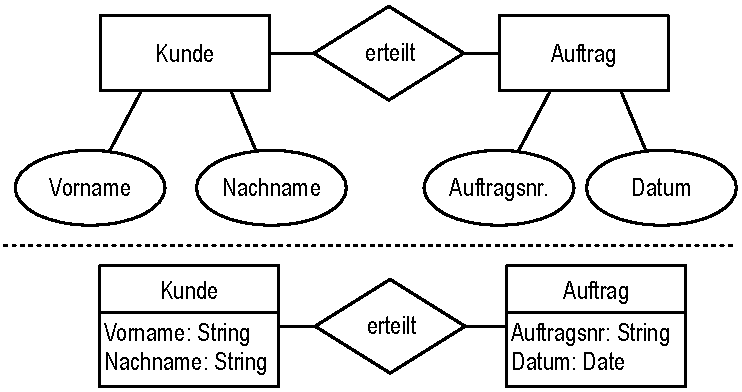
\includegraphics[width=\columnwidth]{figure.pdf}
% \caption{Enter your single-column figure caption here.}
% \label{default}
% \end{figure}
%
% \begin{figure*}[htb]
% \centering
% 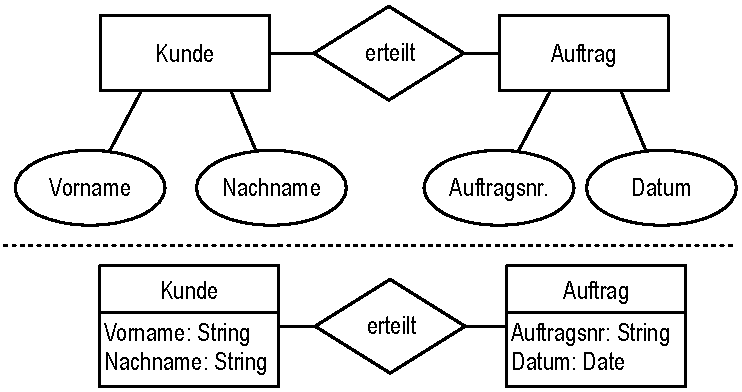
\includegraphics[width=\textwidth]{figure.pdf}
% \caption{Enter your double-column figure caption here.}
% \label{default}
% \end{figure*}
%
% \blindtext
%
%
%
% \subsection{Tables}\label{sec:tables}
% Typeset tables as floats in double-columns using \verb|\begin{table*}|, see Tab.~\ref{tab:unique-label} for an example.
%
% \begin{table*}[tb]
% \centering
% \caption{Enter your table caption above the table here.}
% \begin{tabular}{llllll}
% \toprule
% column head1 & column head2 & column head3 & column head4 & column head5 & column head6\\
% \midrule
% cell1 & cell2 & cell3 & cell4 & cell5 & cell6\\
% cell1 & cell2 & cell3 & cell4 & cell5 & cell6\\
% cell1 & cell2 & cell3 & cell4 & cell5 & cell6\\
% cell1 & cell2 & cell3 & cell4 & cell5 & cell6\\
% cell1 & cell2 & cell3 & cell4 & cell5 & cell6\\
% \bottomrule
% \end{tabular}
% \label{tab:unique-label}
% \end{table*}
%
% %\blindtext[2]\ Lorem ipsum hoc nunc.\footnote{Use footnotes only when absolutely necessary.}
%
%
% %\blindtext[1]
%
%
%
% \section{Formatting the bibliography}\label{sec:bib}
%
% Please make sure to properly enter all data for each entry in the bibliographic database (.bib). Pay special attention to formatting names and page numbers, see Listing~\ref{lst:1} for an example (\cite{key1}) formatted properly in the references section (use \verb|--| between page numbers and \verb|{}| around multiple word surnames!). 
%
% \begin{lstlisting}[float,caption={Enter your single-column listing caption here.},label={lst:1}]
% @ARTICLE{key1,
%   author = {{van der Aalst}, W. M. P. 
%   and {van Hee}, K. M. 
%   and {van Werf}, J. M. 
%   and Verdonk, M.},
%   title = {{Auditing 2.0: Using 
%   Process Mining to Support 
%   Tomorrow's Auditor}},
%   journal = {Computer},
%   year = {2010},
%   volume = {43},
%   pages = {90--93},
%   number = {3}
% }
% \end{lstlisting}
%
%
%
% \section{Source code listings}\label{sec:listings}
%
% For typesetting source code listings, use the \verb|sourcecode|, \verb|java| or \verb|pseudocode| environments provided by the document class. All three environments are customized from the lstlistings package. 
%
% See Listing~\ref{lst:2} for an example of a double-column listing.
%
% \begin{lstlisting}[float=*htbp,caption={Enter your double-column listing caption here. Note that the listing width is too wide. Correct by entering a newline before, \eg, 'Tomorrow'.},label={lst:2}]
% @ARTICLE{key1,
%   author = {{van der Aalst}, W. M. P. and {van Hee}, K. M. and 
%   {van Werf}, J. M. and Verdonk, M.},
%   title = {{Auditing 2.0: Using Process Mining to Support Tomorrow's Auditor}},
%   journal = {Computer},
%   year = {2010},
%   volume = {43},
%   pages = {90--93},
%   number = {3}
% }
% \end{lstlisting}
%
% %\blindtext[3]
%
%
% \section{Formatting pseudocode}\label{sec:algorithm}
% XXX Nutzung von algorithm-Umgebung illustrieren XXX 
%
% \printbibliography
% \end{article}
% \end{document}
% \end{examplecode}
% \clearpage
% \begin{thebibliography}{0}
% 
%   \bibitem{textcomp-pdf}
%     \href
%      {http://www.ctan.org/pkg/textcomp}
%      {Package \pkg{textcomp}:    \LaTeX\  support for the Text Companion fonts}.
% 
% 
%   \bibitem{microtype-pdf}
%     \href
%      {http://www.ctan.org/pkg/microtype}
%      {Package \pkg{microtype}:    An interface to the micro-typographic features of pdf\TeX}.
% 
% 
%   \bibitem{babel-pdf}
%     \href
%      {http://www.ctan.org/pkg/babel}
%      {Package \pkg{babel}:    Multilingual support for Plain \TeX\ or \LaTeX}.
% 
% 
%   \bibitem{float-pdf}
%     \href
%      {http://www.ctan.org/pkg/float}
%      {Package \pkg{float}: 	Improved interface for floating objects}.
% 
% 
%   \bibitem{caption-pdf}
%     \href
%      {http://www.ctan.org/pkg/caption}
%      {Package \pkg{caption}: Customising captions in floating environments}.
% 
% 
%   \bibitem{graphicx-pdf}
%     \href
%      {http://www.ctan.org/pkg/graphicx}
%      {Package \pkg{graphicx}:    Enhanced support for graphics}.
% 
% 
%   \bibitem{xcolor-pdf}
%     \href
%      {http://www.ctan.org/pkg/xcolor}
%      {Package \pkg{xcolor}: 	Driver-independent color extensions for \LaTeX\  and pdf\LaTeX}.
% 
% 
%   \bibitem{biblatex-pdf}
%     \href
%      {http://www.ctan.org/pkg/biblatex}
%      {Package \pkg{biblatex}: Bibliographies in \LaTeX\ using \BibTeX\ for sorting only}.
%  
% 
%   \bibitem{csquotes-pdf}
%     \href
%      {http://www.ctan.org/pkg/csquotes}
%      {Package \pkg{csquotes}: 	Context sensitive quotation facilities}.
% 
% 
%   \bibitem{twoopt-pdf}
%     \href
%      {http://www.ctan.org/pkg/twoopt}
%      {Package \pkg{twoopt}: Definitions with two optional arguments}.
% 
% 
%   \bibitem{environ-pdf}
%     \href
%      {http://www.ctan.org/pkg/environ}
%      {Package \pkg{environ}: 	A new interface for environments in \LaTeX}.
% 
% 
%   \bibitem{paralist-pdf}
%     \href
%      {http://www.ctan.org/pkg/paralist}
%      {Package \pkg{paralist}: 	Enumerate and itemize within paragraphs}.
% 
% 
%   \bibitem{afterpage-pdf}
%     \href
%      {http://www.ctan.org/pkg/afterpage}
%      {Package \pkg{afterpage}: 	Execute command after the next page break}.
% 
% 
%   \bibitem{xspace-pdf}
%     \href
%      {http://www.ctan.org/pkg/xspace}
%      {Package \pkg{xspace}:     Define commands that appear not to eat spaces}.
% 
% 
%   \bibitem{calc-pdf}
%     \href
%      {http://www.ctan.org/pkg/calc}
%      {Package \pkg{calc}:    Simple arithmetic in \LaTeX\  commands}.
% 
% 
%   \bibitem{geometry-pdf}
%     \href
%      {http://www.ctan.org/pkg/geometry}
%      {Package \pkg{geometry}:    Flexible and complete interface to document dimensions}.
% 
% 
%   \bibitem{eso-pic-pdf}
%     \href
%      {http://www.ctan.org/pkg/eso-pic}
%      {Package \pkg{eso-pic}:    Add picture commands (or backgrounds) to every page}.
% 
% 
%   \bibitem{hyperref-pdf}
%     \href
%      {http://www.ctan.org/pkg/hyperref}
%      {Package \pkg{hyperref}:    Extensive support for hypertext in \LaTeX}.
% 
% 
%   \bibitem{source2e-pdf}
%     \href
%      {http://www.tug.org/texlive/Contents/live/texmf-dist/doc/latex/base/source2e.pdf}
%      {The \LaTeXe\ Sources}.
%
% \end{thebibliography}
% \clearpage
% 
% \StopEventually{^^A
%  \PrintChanges
%  \PrintIndex
%}
%
%^^A%%%%%%%%%%%%%%%%%%%%%%%%%%%%%%%%%%%%%%%%%%%%%%%%%%%%%%%%%%%%%%%%%%%%%%%%%%%%
% 
% \section{Implementation}
% \label{sec:code}
% 
% Here, the code of the \LaTeX{} class \cls{\DTXname} begins.
%    \begin{macrocode}
%<*class>
%    \end{macrocode}
%
%^^A%%%%%%%%%%%%%%%%%%%%%%%%%%%%%%%%%%%%%%%%%%%%%%%%%%%%%%%%%%%%%%%%%%%%%%%%%%%%
% 
% \subsection{Options}
% \label{sec:code:opt}
% 
% \begin{option}{british}
%    \begin{macrocode}
\PassOptionsToPackage{british}{babel}
%    \end{macrocode}
% \end{option}
% \begin{option}{draft}
% \begin{option}{final}
% \begin{switch}{@draft}
% If the user requests \opt{draft} we mark any overfull boxes.  There
% is more interesting stuff to be added to this option; one could
% think of altered running titles or watermarks, for example.
%    
% As this option is handed along the package chain it might have other
% effects,~too.
%    \begin{macrocode}
\newif\if@draft
\DeclareOption{draft}{%
  \@drafttrue
  \overfullrule 10pt
}%
\DeclareOption{final}{%
  \@draftfalse
  \overfullrule\z@
}%
%    \end{macrocode}
% \end{switch}
% \end{option}
% \end{option}
% 
% \begin{option}{referee}
% \begin{option}{noreferee}
% \begin{option}{review}
% \begin{option}{noreview}
% \begin{switch}{@referee}
% The options \opt{referee} and \opt{review} switch to \emph{referee mode}.  
% In referee mode some information at the titlepage are removed in order to allow
% an anonymous submission.
%    \begin{macrocode}
\newif\if@referee
\DeclareOption{referee}{\@refereetrue}
\DeclareOption{noreferee}{\@refereefalse}
\DeclareOption{review}{\@refereetrue}
\DeclareOption{noreview}{\@refereefalse}
%    \end{macrocode}
% \end{switch}
% \end{option}
% \end{option}
% \end{option}
% \end{option}
% 
% \begin{option}{cover}
% \begin{option}{nocover}
% \begin{macro}{\coveron}
% \begin{macro}{\coveroff}
% \begin{switch}{@cover}
% Switches cover production on or off.  If \opt{cover} is given then 
% the four cover pages (outer and inner pages of front and back, 
% respectively) are produced and added to the document.
%    \begin{macrocode}
\newif\if@cover
\def\coveron{\@covertrue}
\def\coveroff{\@coverfalse}
\DeclareOption{cover}{\coveron}
\DeclareOption{nocover}{\coveroff}
%    \end{macrocode}
% \end{switch}
% \end{macro}\end{macro}
% \end{option}\end{option}
% 
%    \begin{macrocode}
\newif\if@microtype
\@microtypetrue
\DeclareOption{nomicrotype}{\@microtypefalse}
%    \end{macrocode}
%
% Completing option handling, by now unprocessed option are handed
% over to the base class \cls{article} and the class options list
% is processed from the left to the right.
%    \begin{macrocode}
\PassOptionsToClass{a4paper,twoside,11pt}{article}%
\DeclareOption*{\PassOptionsToClass{\CurrentOption}{article}}%
\ExecuteOptions{final,noreferee,nocover,oneside,openany}%
\ProcessOptions*\relax%
%    \end{macrocode}
% 
%    \begin{macrocode}
\IfFileExists{latexrelease.sty}%
   {\RequirePackage[latest]{latexrelease}}%
   {\RequirePackage{fixltx2e}}%
%    \end{macrocode}
% 
%^^A%%%%%%%%%%%%%%%%%%%%%%%%%%%%%%%%%%%%%%%%%%%%%%%%%%%%%%%%%%%%%%%%%%%%%%%%%%%%
% 
% \subsection{Loading the base class and packages}
% \label{sec:code:cls+pkg}
% 
% This class is build upon the \LaTeX{} standard class \cls{article}.
%    \begin{macrocode}
\LoadClass{article}[2001/06/01]% 
%    \end{macrocode}
% 
%    \begin{macrocode}
\RequirePackage[utf8]{inputenc}%
%    \end{macrocode}
% 
% 
% This loads font definitions for text and mathematics. 
% The package allows the user to select font encodings, and for each
% encoding provides an interface to `font-encoding-specific' commands
% for each font.  Its most powerful effect is to enable hyphenation to
% operate on texts containing any character in the font.
% It is distributed as part of the \LaTeXe{}
% distribution.
%    \begin{macrocode}
\RequirePackage[T1]{fontenc}%
%    \end{macrocode}
% 
% Since many PostScript fonts only implement a subset of the \opt{TS1}
% encoding which contains text symbols for use with the
% \opt{T1}-encoded text fonts, many commands only produce black blobs
% of ink.  The \pkg{textcomp} package is supplied as a part of the
% \LaTeX{} base distribution to resolve the resulting problems~\cite{textcomp-pdf}.
%    \begin{macrocode}
\RequirePackage[full]{textcomp}%
%    \end{macrocode}
% 
% The \pkg{microtype} package provides a \LaTeX{} interface to the
% micro-typographic extensions of pdf\TeX: most prominently, character
% protrusion and font expansion, furthermore the adjustment of
% interword spacing and additional kerning, as well as hyphenatable
% letterspacing (tracking) and the possibility to disable all or
% selected ligatures~\cite{microtype-pdf}.  It allows to apply these features to
% customisable sets of fonts, and to configure all micro-typographic
% aspects of the fonts in a straight-forward and flexible way.
% Settings for various fonts are provided.
%    \begin{macrocode}
\if@microtype
   \RequirePackage{microtype}%
\else
   \ClassWarning{emisa}{Package `microtype` not loaded!%
      \MessageBreak Output will differ from final result in the journal!%
      \MessageBreak Please consult the documentation, if you%
      \MessageBreak get an error when loading microtype}
\fi%   
%    \end{macrocode}
% 
% \pkg{babel} is a package providing an environment in which documents
% can be typeset in a language other than US English, or in more than
% one language~\cite{babel-pdf}.
%    \begin{macrocode}
\RequirePackage{babel}%
%    \end{macrocode}
% 
% This style option improves the interface for defining floating
% objects such as figures and tables in \LaTeX{}~\cite{float-pdf}. It adds the notion of
% a `float style' that governs appearance of floats.  New kinds of
% floats may be defined using a \cs{newfloat} command analogous to
% \cs{newtheorem}.  This style option also incorporates the
% functionality of David Carlisle's style option \pkg{here}, giving
% floating environments a \texttt{[H]} option which means \emph{Put
% it here!} (as opposed to the standard \texttt{[h]} option which
% means \emph{Put it here if possible, or otherwise at the next page if 
% no alternative position is specified.}).
%    \begin{macrocode}
\RequirePackage{float}
%    \end{macrocode}
% 
% The \pkg{caption} package gives the user the possibility to control the look
% \& feel of the captions from floating environments like \env{figure} and
% \env{table}. Furthermore it does similar to the caption stuff coming from
% other packages (like the \pkg{longtable} or \pkg{supertabular} package)~\cite{caption-pdf}.
% 
% For more information on that see the
% \href{http://ctan.tug.org/tex-archive/macros/latex/contrib/caption/caption-eng.pdf}{english},
% \href{http://ctan.tug.org/tex-archive/macros/latex/contrib/caption/caption-rus.pdf}{russian}, or
% \href{http://dante.ctan.org/tex-archive/macros/latex/contrib/caption/caption-deu.pdf}{german} user documentation.
%
%    \begin{macrocode}
\RequirePackage[font={small}]{caption}
%    \end{macrocode}
% 
% 
% 
%^^A%%%%%%%%%%%%%%%%%%%%%%%%%%%%%%%%%%%%%%%%%%%%%%%%%%%%%%%%%%%%%%%%%%%%%%%%%%%%
% 
% \subsubsection{Colour and graphics}
% 
% \pkg{graphicx} as part of the graphics package provides a
% key-value interface for optional arguments to the
% \cs{includegraphics} command~\cite{graphicx-pdf}.
%    \begin{macrocode}
\RequirePackage{graphicx}%
%    \end{macrocode}
% 
% The package \pkg{xcolor} is a color extension
% for \LaTeX{} and pdf\LaTeX{} that provides easy driver-independent
% access to several kinds of colors, tints, shades, tones, and mixes
% of arbitrary colors by means of color expressions~\cite{xcolor-pdf}.
% \iffalse
% It allows to select a document-wide target color model and offers tools for
% \begin{itemize}
%   \item automatic color schemes,
%   \item conversion between twelve (sic!) color models (rgb, cmy, cmyk, hsb,
%     Hsb, tHsb, gray, RGB, HTML, HSB, Gray, wave)
%   \item alternating table row colors,
%   \item color blending,
%   \item color masking,
%   \item color separation, and
%   \item color wheel calculations.
% \end{itemize}
% \fi
%    \begin{macrocode}
\RequirePackage[fixinclude,table]{xcolor}%
%    \end{macrocode}
% 
% 
% The \pkg{biblatex} package~\cite{biblatex-pdf} is a complete reimplementation of the
% bibliographic facilities provided by \LaTeX{} in conjunction with
% \BibTeX. It redesigns the way in which \LaTeX{} interacts with BibTeX at
% a fairly fundamental level. With \pkg{biblatex}, \BibTeX{} is only used to
% sort the bibliography and to generate labels. Instead of being
% implemented in \BibTeX{}'s style files, the formatting of the
% bibliography is entirely controlled by \TeX{} macros. Good working
% knowledge in \LaTeX{} should be sufficient to design new bibliography
% and citation styles. There is no need to learn \BibTeX{}'s postfix stack
% language. Just like the bibliography styles, all citation commands
% may be freely (re)defined.
% 
% Apart from the features unique to \pkg{biblatex}, the package also
% incorporates core features of the following packages: \pkg{babelbib},
% \pkg{backref}, \pkg{bibtopic}, \pkg{bibunits}, \pkg{chapterbib}, \pkg{cite},
% \pkg{citeref}, \pkg{inlinebib}, \pkg{mlbib}, \pkg{multibib}, \pkg{natbib},
% \pkg{splitbib}. There are also some conceptual parallels to the \pkg{amsrefs}
% package. The \pkg{biblatex} package supports split bibliographies, multiple
% bibliographies within one document, and separate lists of bibliographic
% shorthands. Bibliographies may be subdivided into parts (by chapter, by
% section, etc.) and/or segmented by topics (by type, by keyword, etc.). The
% package is fully localized and can interface with the \pkg{babel} package.
% 
% This package requires e-\TeX{} and the \pkg{etoolbox} package. Installing
% the \pkg{csquotes} package is recommended.
%    \begin{macrocode}
\RequirePackage{etoolbox}%
%    \end{macrocode}
% 
% We use it with these options:
% \begin{compactdesc}
%   \item{\opt{style=emisa}} sets the base name of the bibliography and 
%   citation format files; thus we use \file{emisa.bbx} and 
%   \file{emisa.cbx} that are defined below.
%   \item{\opt{natbib=true}} enables the use of \pkg{natbib} citation 
%   commands with \pkg{biblatex}.
%   \item{\opt{maxcitenames=3}} Author lists with more than two entries are 
%   abbreviated with ``et al.''.  Note that in the bibliography 
%   listing  author lists won't be shortened at all.\footnote{That is, 
%   they \emph{will} be shortened if there are more than 999 
%   authors.  That should occur not that often, though.}
%   \item{\opt{terseinits}} If Initials are given with (false) or
%   without (true) punctuation and whitespace.
%   \item{\opt{isbn=false}} In bibliographies, no ISBNS, \ldots
%   \item{\opt{url=false}} \ldots\ no URLs, \ldots
%   \item{\opt{doi=false}} \ldots\ no DOIs, \ldots
%   \item{\opt{eprint=false}} \ldots\ and no ePrint marks are   displayed.
%   \item{\opt{dashed=false}} Identical author entries of consecutive
%   bibliography entries don't get replaced by a dash (beginning with the second one).
% \end{compactdesc}
% 
%    \begin{macrocode}
\RequirePackage[%
    style=emisa,%
    natbib=true,%
    backend=biber,%
]{biblatex}
%    \end{macrocode}
% 
%    \begin{macrocode}
\ExecuteBibliographyOptions{%
   maxcitenames=3,%
   maxbibnames=999,%
   terseinits=false,%
   isbn=false,%
   url=true,%
   doi=false,%
   eprint=false,%
   dashed=false,%
   bibencoding=inputenc,%
   sorting=anyt,%
   hyperref=true%
}%
%    \end{macrocode}
% 
% This package provides advanced facilities for inline and display
% quotations~\cite{csquotes-pdf}.  
% \iffalse
% It is designed for a wide range of tasks ranging from
% the most simple applications to the more complex demands of formal
% quotations.  The facilities include commands, environments, and
% user"=definable \enquote*{smart quotes} which dynamically adjust to their
% context.  
% \fi
% Quotation marks are switched automatically if quotations
% are nested and can adjust to the current language.  There are
% additional facilities designed to cope with the more specific
% demands of academic writing, especially in the humanities and the
% social sciences.  All quote styles as well as the optional active
% quotes are freely configurable.
%    \begin{macrocode}
\RequirePackage[babel=once,english=british]{csquotes}
%    \end{macrocode}
% 
% 
% 
%^^A%%%%%%%%%%%%%%%%%%%%%%%%%%%%%%%%%%%%%%%%%%%%%%%%%%%%%%%%%%%%%%%%%%%%%%%%%%%%
% 
% \subsubsection{Helpers}
% \label{sec:code:cls+pkg:helpers}
% 
% \pkg{twoopt} provides commands to define macros with \emph{two}
% optional parameters.  This package is part of the \emph{Oberdiek}
% bundle~\cite{twoopt-pdf}.
%    \begin{macrocode}
\RequirePackage{twoopt}%
%    \end{macrocode}
% 
% 
% \pkg{environ} provides a new method of defining
% environments~\cite{environ-pdf}.
%    \begin{macrocode}
\RequirePackage{environ}%
%    \end{macrocode}
% 
% \pkg{paralist} provides a few new list environments. Itemized and enumerated 
% lists can be typesetted within paragraphs, as paragraphs and in a compact
% version. Most environments have optional arguments to format the labels.
% Additionally, the \LaTeX{} environments itemize and enumerate can be 
% extended to use a similar optional argument~\cite{paralist-pdf}.
% 
% The options' meanings are as follows:
% \begin{description}
% \item{\opt{neveradjust}\quad} The width of the labels is never
% adjusted, not even for environments where you defined the labels
% manually using the optional argument.
% \item{\opt{defblank}\quad} The two environments \env{inparablank} 
% and \env{asparablank} will be defined.
% \item{\opt{flushright}\quad} The labels in the four lists mentioned
% above are set flush right.
% \end{description}
%    \begin{macrocode}
\RequirePackage[neveradjust,defblank,flushright]{paralist}%
%    \end{macrocode}
% 
% We make the traditional list environments equal the compact ones so 
% there is no visual difference and they are both modifiable easily.
%    \begin{macrocode}
\let\itemize\compactitem
\let\enditemize\endcompactitem
\let\enumerate\compactenum
\let\endenumerate\endcompactenum
\let\description\compactdesc
\let\enddescription\endcompactdesc
%    \end{macrocode}
% 
% 
% These macros are imported from \pkg{paralist}, setting standard
% enumeration marks and list indentations.
% \changes{0.95i}{2011/04/06}{Default left margin in all levels of
% all list environments set to 1.25em.}
% \changes{0.95l}{2012/12/11}{Default left margin setting changed back to old
% setting after production-level \file{emisa.cfg}:
% 1em/0.9em/0.7em/0.5em/0.4em/0.3em.}
% \changes{2.0}{2015/12/21}{No more config files}
% \changes{2.0}{2015/12/21}{pltopsep changed}
%    \begin{macrocode}
\setdefaultenum{1.}{a)}{i.}{A}% 
\setdefaultleftmargin{1em}{0.9em}{0.7em}{0.5em}{0.4em}{0.3em}%
\setlength{\plitemsep}{3\p@}%
\setlength{\pltopsep}{6\p@}
%    \end{macrocode}
% 
% \pkg{afterpage} implements a command that causes the commands
% specified in its argument to be expanded after the current page is
% output~\cite{afterpage-pdf}.
% 
% The \pkg{xspace} package provides a single command that looks
% at what comes after it in the command stream, and decides whether to
% insert a space to replace one ``eaten'' by the \TeX{} command decoder.
% The decision is based on what came after any space, not on whether
% there was a space (which is unknowable): so if the next thing proves
% to be punctuation, the chances are there was no space, but if it's a
% letter, there's probably a need for space~\cite{xspace-pdf}.
% 
% \pkg{calc} adds infix expressions to perform arithmetic on the
% arguments of the \LaTeX{} commands \cs{setcounter}, \cs{addtocounter},
% \cs{setlength}, and \cs{addtolength}~\cite{calc-pdf}.
% 
% All three packages are part of the tools bundle in the \LaTeX{} required
% distribution.
%    \begin{macrocode}
\RequirePackage{afterpage,xspace,calc}%
%    \end{macrocode}
% 
% 
% 
% \pkg{geometry} provides an easy and flexible user interface to
% customize page layout, implementing auto-centering and
% auto-balancing mechanisms so that the users have only to give the
% least description for the page layout~\cite{geometry-pdf}.
% 
% An important feature is the package's ability to communicate the
% paper size it's set up to the output (whether via DVI \cs{special}s
% or via direct interaction with pdf\LaTeX{}).
%    \begin{macrocode}
\RequirePackage{geometry}%
%    \end{macrocode}
% 
% \pkg{eso-pic} adds one or more user commands to \LaTeX{}'s shipout
% actions, making it easy to add some picture commands to any and
% every page at absolute positions~\cite{eso-pic-pdf}.
%    \begin{macrocode}
\RequirePackage{eso-pic}%
%    \end{macrocode}
% 
% 
% 
%^^A%%%%%%%%%%%%%%%%%%%%%%%%%%%%%%%%%%%%%%%%%%%%%%%%%%%%%%%%%%%%%%%%%%%%%%%%%%%%
% 
% \subsubsection{Scripts, fonts, and maps}
% 
%    \begin{macrocode}
\RequirePackage{newtxtext}
\RequirePackage{newtxmath}
\RequirePackage[zerostyle=b,straightquotes]{newtxtt}
\if@microtype
   \UseMicrotypeSet[protrusion]{basicmath} % disable protrusion for tt fonts
\fi%
%    \end{macrocode}
% 
% To make figures and ligatures searchable when using pdf\TeX${}\geq 1.40$,
% glyph-to-unicode translation must be enabled.  The default table
% \file{glyphtounicode.tex} contains mappings from glyph names to
% corresponding unicode for embedded fonts.  It covers the AGL (Adobe
% Glyph List), names from \file{texglyphlist.txt} (part of
% \textsf{lcdf}-typetools) and \file{zapfdingbats.txt}, plus a
% few~exceptions.
%    \begin{macrocode}
\InputIfFileExists{glyphtounicode}%
   {\ClassInfo{emisa}{Reading file `glyphtounicode.tex`}
    \pdfgentounicode=1}%
   {\ClassWarning{emisa}{Couldn't find file `glyphtounicode.tex`}}%
%    \end{macrocode}
%
%    \begin{macrocode}
   \RequirePackage{booktabs}
   \RequirePackage{listings}
   \lstset{basicstyle=\ttfamily\small}
   \RequirePackage{amsmath}
   \RequirePackage[amsmath,standard,hyperref]{ntheorem}
%    \end{macrocode} 
% 
%^^A%%%%%%%%%%%%%%%%%%%%%%%%%%%%%%%%%%%%%%%%%%%%%%%%%%%%%%%%%%%%%%%%%%%%%%%%%%%%
% 
% \subsection{Hypertext}
% \label{sec:code:hypertext}
% 
% The \pkg{hyperref} package~\cite{hyperref-pdf} has to loaded as late as feasible so it 
% can intercept changes to standard macros by other packages.
%    \begin{macrocode}
\RequirePackage{url}
\urlstyle{same}
\RequirePackage[%
  colorlinks,
  breaklinks,
  pdfview=Fit,
  bookmarksopen,
  bookmarksnumbered,
  linkcolor=black,
  anchorcolor=black,
  citecolor=black,
  filecolor=black,
  urlcolor=black,
  hyperfootnotes=false
  ]{hyperref}%
%    \end{macrocode}
%
%    \begin{macrocode}
\RequirePackage{doclicense}
%    \end{macrocode} 
% 
%^^A%%%%%%%%%%%%%%%%%%%%%%%%%%%%%%%%%%%%%%%%%%%%%%%%%%%%%%%%%%%%%%%%%%%%%%%%%%%%
% 
% \subsection{Tools}
% \label{sec:code:tools}
% 
% \begin{macro}{\@ifempty}
% \begin{macro}{\@ifarg}
% \begin{macro}{\@ifnoarg}
% These determinate if an argument ist empty (or not) and to act consequently.
% An argument is \glq{}empty\grq{}, iff it contains nothing or just whitespace.
% All three macros first test their first argument. If it is empty \cs{@ifempty}
% then executes the second one, otherwise the third one. \cs{@ifnoarg} und
% \cs{@ifarg} execute their respective second argument iff the the first one is
% (not) empty.
% \begin{syntax}
% \cs{@ifempty}\marg{arg}\marg{Action\_if\_empty}\marg{Action\_if\_not\_empty}\\
% \cs{@ifnoarg}\marg{arg}\marg{Action\_if\_empty}\\
% \cs{@ifarg}\marg{arg}\marg{Action\_if\_not\_empty}\\
% \end{syntax}
%    \begin{macrocode}
\begingroup
  \catcode`\Z=3
  \long\gdef\@M@T@#1#2Z#3#4#5\@nil{#4}
  \long\gdef\@ifempty#1{\@M@T@#1ZZ\@secondoftwo\@firstoftwo\@nil}
  \long\gdef\@ifarg#1{\@M@T@#1ZZ\@firstofone\@gobble\@nil}
  \long\gdef\@ifnoarg#1{\@M@T@#1ZZ\@gobble\@firstofone\@nil}
\endgroup
%    \end{macrocode}
% \end{macro}
% \end{macro}
% \end{macro}
% 
%
%
% 
% 
%^^A%%%%%%%%%%%%%%%%%%%%%%%%%%%%%%%%%%%%%%%%%%%%%%%%%%%%%%%%%%%%%%%%%%%%%%%%%%%%
% 
% \subsection{Basic page layout}
% \label{sec:code:pagelayout}
% 
% The \pkg{geometry} options using the keyval
% (\meta{key}\,=\,\meta{value}) interface can be set either in the
% optional argument to the \cs{usepackage} command, or in the argument
% of the \cs{geometry} macro.  In either case, the argument consists
% of a list of comma-separated keyval options.  \cs{geometry} acts
% cumulative; so multiple use just appends options to the list.
%    \begin{macrocode}
\geometry{%
  a4paper,%
  portrait,%
  twoside,%
  ignoreall,%
  hcentering,%
  textwidth      = 162.5mm,%
  textheight     = 220mm,%
  heightrounded,%
  columnsep      = 12.5mm,%
  top            = 47mm,%
  headheight     = 16mm,%
  headsep        = 13mm,%
  marginparwidth = 15mm,%
  marginparsep   = 5mm,%
  footskip       = 16mm%
  }%
\marginparpush 5mm%
%    \end{macrocode}
% 
% 
%    \begin{macrocode}
\AtBeginDocument{\baselineskip=13.6pt plus 0.5pt}%
%    \end{macrocode}
% 
% 
%    \begin{macrocode}
\parindent=4mm%
%    \end{macrocode}
% 
% 
%    \begin{macrocode}
\smallskipamount=.5\baselineskip
\medskipamount=2\smallskipamount
\bigskipamount=2\medskipamount
%    \end{macrocode}
% 
% 
%    \begin{macrocode}
\flushbottom 
%    \end{macrocode}
% 
% 
%    \begin{macrocode}
\abovedisplayskip=.5\baselineskip plus .33\baselineskip 
                                  minus .33\baselineskip
\belowdisplayskip=\abovedisplayskip
\abovedisplayshortskip= 0pt plus .33\baselineskip
\belowdisplayshortskip=.5\baselineskip plus .33\baselineskip 
                                       minus .33\baselineskip
%    \end{macrocode}
% 
% 
% 
%^^A%%%%%%%%%%%%%%%%%%%%%%%%%%%%%%%%%%%%%%%%%%%%%%%%%%%%%%%%%%%%%%%%%%%%%%%%%%%%
% 
% \subsection{Scripts}
% \label{sec:code:scripts}
% 
% \begin{macro}{\pageheadfont}
% \begin{macro}{\pagenumfont}
% \begin{macro}{\pagefootfont}
% Assigning scripts to text elements.\\
% Page head and foot:
%    \begin{macrocode}
\def\pageheadfont{\normalfont}%
\def\pagenumfont{\pageheadfont\bfseries}%
\def\pagefootfont{\pageheadfont}%
%    \end{macrocode}
% \end{macro}\end{macro}\end{macro}
% 
% \begin{macro}{\authorfont}
% \begin{macro}{\titlefont}
% \begin{macro}{\subtitlefont}
% \begin{macro}{\abstractfont}
% The elements of the article titles:
%    \begin{macrocode}
\def\authorfont{\normalfont\Large}%    
\def\titlefont{\normalfont\bfseries\LARGE\boldmath}%    
\def\subtitlefont{\normalfont\bfseries\Large\boldmath}%    
\def\abstractfont{\normalfont\itshape}%    
%    \end{macrocode}
% \end{macro}\end{macro}
% \end{macro}\end{macro}
% 
% \begin{macro}{\affiliationfont}
% \begin{macro}{\affiliationauthorfont}
% \begin{macro}{\affiliationaddressfont}
% \begin{macro}{\affiliationemailfont}
% The elements of the affiliation box:
%    \begin{macrocode}
\def\affiliationfont{\normalfont}
\def\affiliationauthorfont{\bfseries}
\def\affiliationaddressfont{\mdseries}
\def\affiliationemailfont{\mdseries}%    
%    \end{macrocode}
% \end{macro}\end{macro}
% \end{macro}\end{macro}
% 
% \begin{macro}{\sectionfont}
% \begin{macro}{\sec@font}
% \begin{macro}{\para@font}
% Section headlines:
% \label{sec:code:scripts-sec@font}
%    \begin{macrocode}
\def\sectionfont{%
  \normalfont
  \bfseries   
  \boldmath}%
\def\sec@font{\sectionfont\large}%
\def\para@font{\sectionfont}%
%    \end{macrocode}
% \end{macro}
% \end{macro}
% \end{macro}
% 
% \begin{macro}{\captionfont}
% Captions:
%    \begin{macrocode}
\def\captionfont{\normalfont\small\itshape}
%    \end{macrocode}
% \end{macro}
% 
% 
%^^A%%%%%%%%%%%%%%%%%%%%%%%%%%%%%%%%%%%%%%%%%%%%%%%%%%%%%%%%%%%%%%%%%%%%%%%%%%%%
% 
% \subsection{Colours}
% \label{sec:code:color}
% 
% These are the colour definitions for a couple of elements.
% \begin{colordef}{coverbgcolor}
% \begin{colordef}{covertextcolor}
% The colours of the cover background (near 25\% grey) and cover 
% text (such as headlines, near 75\%~
% grey):
%    \begin{macrocode}
\definecolor{coverbgcolor}{cmyk}{0.15,0.1,0.09,0}%
\definecolor{covertextcolor}{cmyk}{0.77,0.76,0.70,0.61}%
%    \end{macrocode}
% \end{colordef}
% \end{colordef}
% 
% 
% \begin{colordef}{headtextcolor}
% \begin{colordef}{boxframecolor}
% \begin{colordef}{boxbgcolor}
% These are the colours of the grey elements in column titles (50\% 
% grey) and of the frame and the background of text boxes like that one used in 
% \cs{editorialboard} (100\% grey~= black and 20\% grey, respectively). 
%    \begin{macrocode}
\definecolor{headtextcolor}{gray}{0.5}%
\definecolor{boxframecolor}{gray}{1}%
\definecolor{boxbgcolor}{gray}{0.8}%
%    \end{macrocode}
% \end{colordef}
% \end{colordef}
% \end{colordef}
% 
% 
%^^A%%%%%%%%%%%%%%%%%%%%%%%%%%%%%%%%%%%%%%%%%%%%%%%%%%%%%%%%%%%%%%%%%%%%%%%%%%%%
% 
% \subsection{Double line spacing}
% \label{sec:code:referee}
%
% \begin{macro}{\displayskipstretch}
% \begin{macro}{\setdisplayskipstretch}
%    \begin{macrocode}
\newcommand{\displayskipstretch}{\baselinestretch}
\newcommand{\setdisplayskipstretch}[1]{\def\displayskipstretch{#1}}
%    \end{macrocode}
% \end{macro}
% \end{macro}
%
% \begin{macro}{\setstretch}
%  Line space commands.
%    \begin{macrocode}
\newcommand{\setstretch}[1]{%
  \def\baselinestretch{#1}%
  \@currsize
}
%    \end{macrocode}
% \end{macro}
%
% \begin{macro}{\@setsize}
% Modification of the LaTeX command \cs{@setsize}.
% Stretch the baseline \emph{before} calculating the strut size.  This
% improves spacing below tabular environments etc., probably.
% 
% The meanings of the arguments to \cs{@setsize}
% appear to be (whatever these may signify):
% \begin{syntax}
%   \cs{@setsize}\marg{current size}\marg{font baselineskip}\marg{ignored (!)}\marg{font size}
% \end{syntax}
% 
% Note that \cs{@setsize} (in modern \LaTeX{}, \cs{@setfontsize}, which
% is called by \cs{@setsize}) seems to be the only place in purely
% modern LaTeX where \cs{@currsize} is set, and \file{ltxguide.cls}
% seems to be the only file in the LaTeX base distribution that uses
% it.
%    \begin{macrocode}
\def\@setsize#1#2#3#4{%
  \@nomath#1%
  \let\@currsize#1%
  \baselineskip #2%
  \baselineskip=\baselinestretch\baselineskip
  \parskip=\baselinestretch\parskip
  \setbox\strutbox \hbox{%
    \vrule height.7\baselineskip
           depth.3\baselineskip
           width\z@}%
  \skip\footins=\baselinestretch\skip\footins
  \normalbaselineskip\baselineskip#3#4}
%    \end{macrocode}
% \end{macro}
%
% Fix up spacing before and after displayed math
% (arraystretch seems to do a fine job for inside LaTeX displayed math,
% since array and eqnarray seem to be affected as expected).
%    \begin{macrocode}
\everydisplay\expandafter{%
  \the\everydisplay
  \abovedisplayskip   \displayskipstretch\abovedisplayskip
  \belowdisplayskip   \displayskipstretch\belowdisplayskip
  \abovedisplayshortskip  \displayskipstretch\abovedisplayshortskip
  \belowdisplayshortskip  \displayskipstretch\belowdisplayshortskip
}
%    \end{macrocode}
%
% 
% 
% 
%^^A%%%%%%%%%%%%%%%%%%%%%%%%%%%%%%%%%%%%%%%%%%%%%%%%%%%%%%%%%%%%%%%%%%%%%%%%%%%%
% 
% \subsection{Document markup}
% \label{sec:code:markup}
%
% 
%^^A%%%%%%%%%%%%%%%%%%%%%%%%%%%%%%%%%%%%%%%%%%%%%%%%%%%%%%%%%%%%%%%%%%%%%%%%%%%%
% 
% \subsubsection{Declaring issue data}
% \label{sec:code:markup:issuedata}
% 
% The following macros save their argument(s) to internal variables 
% for later usage: 
% \begin{macro}{\journalname}
% The journal name.
%    \begin{macrocode}
\def\journalname#1{\@bsphack\def\@journalname{#1}\@esphack}%
\journalname{Enterprise Modelling and Information Systems Architectures}%
%    \end{macrocode}
% \end{macro}
%
% \begin{macro}{\issn}
% The International Standard Serial Number (ISSN) is the standardized
% international code which allows the identification of any serial
% publication, including electronic serials, independently of its
% country of publication, of its language or alphabet, of its
% frequency, medium, etc.; see the 
% \href{http://www.issn.org/}{ISSN~web~site}.
% 
% Here we have two of them, one for print and one for online issues.
%    \begin{macrocode}
\long\def\issn#1{\@bsphack\long\def\@issn{#1}\@esphack}%
\issn{%ISSN 1860-6059 (Print)\par
      ISSN 1866-3621 (Online)}%
%    \end{macrocode}
% \end{macro}
%
% \begin{macro}{\volume}
% Volume number.
%    \begin{macrocode}
\def\volume#1{\@bsphack\def\@volume{#1}\@esphack}%
\volume{\textcolor{red}{0}}%
%    \end{macrocode}
% \end{macro}
% 
% \begin{macro}{\issue}
% Issue number and date.
%    \begin{macrocode}
\def\issue#1#2{\@bsphack
  \def\@issue{#1}%
  \def\@issuedate{#2}%
  \@esphack}%
\issue{\textcolor{red}{0}}{\textcolor{red}{month 0000}}%
%    \end{macrocode}
% \end{macro}
% 
% \begin{macro}{\specialissuetitle}
% \changes{0.92n}{2010/05/18}{Fixed missing \cs{space} after 
% non-empty Special Issue title 
% prefix.}
% \begin{macro}{\specialissuetitle*}
% \changes{0.92n}{2010/05/18}{New.}
% \begin{macro}{\specialissuetitleprefix}
% If the current issue is a \emph{special issue}, the respective 
% title goes here.
%    \begin{macrocode}
\def\specialissuetitle{\@ifstar\@sspit\@spit}%
\newcommand{\@spit}[2][]{%
  \@bsphack
  \@ifempty{#2}%
   {\let\@specialissuetitle\relax}%
   {\@ifempty{#1}%
     {\def\@specialissuetitle{\@specialissuetitleprefix#2}}%
     {\def\@specialissuetitle{#1\space#2}}}%
  \@esphack}%
\newcommand{\@sspit}[2][]{%
  \@bsphack
  \@ifempty{#2}%
   {\let\@specialissuetitle\relax}%
   {\def\@specialissuetitle{#2}}%
  \@esphack}%
\newcommand{\specialissuetitleprefix}[1]{%
  \@bsphack
  \@ifempty{#1}%
     {\let\@specialissuetitleprefix\relax}%
     {\def\@specialissuetitleprefix{#1\space}}%
  \@esphack}%
\specialissuetitle{}%
\specialissuetitleprefix{Special Issue on}%
%    \end{macrocode}
% \end{macro}
% \end{macro}
% \end{macro}
% 
% \begin{macro}{\copyrightyear}
% \begin{macro}{\copyrightholder}
% Copyright owner and year.
%    \begin{macrocode}
\def\copyrightyear#1{\@bsphack\def\@copyrightyear{#1}\@esphack}%
\copyrightyear{\the\year}%
\def\copyrightholder#1{\@bsphack\def\@copyrightholder{#1}\@esphack}%
\copyrightholder{\textcolor{red}{\copyright{}holder}}%
%    \end{macrocode}
% \end{macro}
% \end{macro}
%
%
% \begin{macro}{\title}
% \begin{macro}{\subtitle}
% \begin{macro}{\author}
% Title, subtitle, and author information for the 
% current article.
% 
% These macros are a bit special as they accept up to \emph{two}
% optional arguments together with the obligatory one.  The optional
% arguments are for the running-title (\emph{short}) and the
% table-of-contents (\emph{ToC}) versions, respectively, of the main
% entry, if there is any:
% \begin{syntax}
% \cs{title}\oarg{short\_title}\oarg{ToC\_title}\marg{title}\\
% \cs{subtitle}\oarg{short\_subtitle}\oarg{ToC\_subtitle}\marg{subtitle}\\
% \cs{author}\oarg{short\_author}\oarg{ToC\_author}\marg{author}\\
% \end{syntax}
% 
% If \emph{no} optional argument is given the obligatory argument 
% will appear in all the respective places.
% 
% If \emph{one} optional argument is given then its' value replaces 
% both the \emph{short} and the \emph{ToC} entries.
% 
% If \emph{two} optional arguments are given then the value of the
% first one becomes the \emph{short} headline (et al.)  entry, and 
% the second one is reproduced in the table of contents.
% 
% If \emph{both} optional arguments are given but the
% first one is left empty then the \emph{short} entry defaults also 
% to the main value, and only the \emph{ToC} entry is changed.
%    \begin{macrocode}
\renewcommandtwoopt*{\title}[3][][]{%
  \@bsphack
  \def\@title{#3}%
  \@ifempty{#1}{\def\@shorttitle{\@title}}{\def\@shorttitle{#1}}%
           \@ifempty{#2}{\def\@toctitle{\@shorttitle}}{\def\@toctitle{#2}}%
  \@esphack}%
\newcommandtwoopt*{\subtitle}[3][][]{%
  \@bsphack
  \def\@subtitle{#3}%
  \@ifempty{#1}{\def\@shortsubtitle{\@subtitle}}{\def\@shortsubtitle{#1}}%
  \@ifempty{#2}{\def\@tocsubtitle{\@shortsubtitle}}{\def\@tocsubtitle{#2}}%
  \@esphack}%
\def\email#1{%
   \ifx\@email\@empty
      \def\@email{#1}
   \else
      \ClassError{emisa}{There can only be one corresponding author!}{}
   \fi}%  
\renewcommand{\author}{\@ifstar{\@authorstar}{\@authornostar}}
\newcommand*{\@authornostar}[1]{%
  \@bsphack
  \if@referee
    \def\@authors{}%
    \def\@shortauthors{}
  \else
      \gdef\@address@sep{}%
      \ifx\@authors\@empty
          \protected@xdef\@authors{#1}
          \protected@xappto\@shortauthors{#1}
      \else
          \protected@xappto\@authors{,\space #1}
          \protected@xappto\@shortauthors{,\space #1}
      \fi%
  \fi
  \@esphack}%
\newcommandtwoopt*{\@authorstar}[3][][]{%
    \@bsphack
    \if@referee
      \def\@authors{}%
      \def\@shortauthors{}%
      \def\@tocauthors{}%
      \def\@email{}%
    \else
      \gdef\@address@sep{}%
      \ifx\@authors\@empty
          \protected@xdef\@authors{#3\textsuperscript{*,}}
          \protected@xappto\@shortauthors{#3}
      \else
          \protected@xappto\@authors{,\space #3\textsuperscript{*,}}
          \protected@xappto\@shortauthors{,\space #3}
      \fi%
      \@ifempty{#1}{\def\@shortauthor{\@shortauthors}}{\def\@shortauthor{#1}}%
      \@ifempty{#2}{\def\@tocauthor{\@shortauthors}}{\def\@tocauthor{#2}}%
    \fi
    \@esphack
    \@ifnextchar\bgroup\email{\ClassError{emisa}{Please provide an E-mail address for the corresponding author}{Use the second argument for the E-mail address}}}%
\newcommand{\keywords}[1]{
   \@bsphack
   \def\and{\unskip\ \textbullet\ }%
   \def\@keywords{#1}%
   \@esphack}%
\newcommand{\authornote}[1]{
   \@bsphack
   \def\@authornote{#1}%
   \@esphack}%
\newcommand{\editor}[1]{
   \@bsphack
   \def\@articleinfo@name{#1}%
   \@esphack}%
\newcommand{\received}[1]{
   \@bsphack
   \def\@articleinfo@rdate{#1}%
   \@esphack}%
\newcommand{\accepted}[2][]{
   \@bsphack
   \def\@articleinfo@rounds{#1}
   \def\@articleinfo@adate{#2}%
   \@esphack}%
\newcommand{\doitext}{DOI:}
\newcommand*{\outdoi}{% 
  \begingroup 
  \lccode`\~=`\#\relax 
  \lowercase{\def~{\#}}%
  \lccode`\~=`\_\relax
  \lowercase{\def~{\_}}%
  \lccode`\~=`\<\relax 
  \lowercase{\def~{\textless}}%
  \lccode`\~=`\>\relax 
  \lowercase{\def~{\textgreater}}%
  \lccode`\~=0\relax 
  \catcode`\#=\active 
  \catcode`\_=\active 
  \catcode`\<=\active 
  \catcode`\>=\active 
  \@outdoi
}
\def\@outdoi#1{% 
  \let\#\relax
  \let\_\relax
  \let\textless\relax 
  \let\textgreater\relax 
  \edef\x{\toks0={{#1}}}% 
  \x
  \edef\#{\@percentchar23}%
  \edef\_{_}%
  \edef\textless{\@percentchar3C}% instead of {\string<} for Apple
  \edef\textgreater{\@percentchar3E}% instead of {\string>} for Apple
  \edef\x{\toks1={\noexpand\href{http://dx.doi.org/#1}}}% 
  \x
  \edef\x{\endgroup\doitext\the\toks1 \the\toks0}%
  \x
}
\newcommand*{\doi}[1]{
   \@bsphack
   \def\@doi{#1}
   \@esphack}%
\newcommand{\acknowledgements}[1]{
   \@bsphack
   \def\@acknowledgements{#1}
   \@esphack}%
\newif\if@licenseset
\newcommand{\licence}[1]{%
   \@bsphack
   \def\@licence{#1}
   \@esphack}%
\let\license\licence
\newcommand{\CCBYNCSAThree}{%
   \@licensesettrue%
   \def\doclicense@type{CC}%
   \def\doclicense@modifier@uppercase{BY-NC-SA}%
   \def\doclicense@versionUsed{3.0}%
}%
\newcommand{\CCBYNCSAFour}{%
   \@licensesettrue%
   \def\doclicense@type{CC}%
   \def\doclicense@modifier@uppercase{BY-NC-SA}%
   \def\doclicense@versionUsed{4.0}%
}%
\newcounter{addresses}
\renewcommand{\theaddresses}{\alph{addresses}}
\newcommand{\address}[2][]{%
  \@bsphack
  \if@referee
     \def\@addresses@list{}
  \else
      \@ifempty{#2}{%
          \@ifempty{#1}{}{%
               \protected@xappto\@authors{\textsuperscript{\@address@sep #1}}
               \gdef\address@sep{,}%
       }}{%
            \stepcounter{addresses}
            \protected@xappto\@authors{\textsuperscript{\@address@sep\theaddresses}}
            \gdef\@address@sep{,}%
            \ifx\@addresses@list\@empty
                \protected@xdef\@addresses@list{\textsuperscript{\theaddresses}\ #2}
            \else
                \protected@xappto\@addresses@list{\newline\textsuperscript{\theaddresses}\ #2}
            \fi}
  \fi
  \@esphack}%
\title{}%
\subtitle{}%
\author{}%
\address{}
\keywords{}%
\authornote{}%
\editor{}%
\received{}%
\accepted{}%
\doi{}%
\licence{}
\acknowledgements{}%
\def\abstract#1{\@bsphack\def\@abstract{#1}\@esphack}%
\abstract{}%
\def\@authors{}
\def\@shortauthor{}
\def\@shortauthors{}
\def\@tocauthor{}
\def\@tocauthors{}
\def\@email{}
\def\@addresses@list{}
%    \end{macrocode}
% \end{macro}
% \end{macro}
% \end{macro}
%  
% \begin{macro}{\abstract}
%    This accepts the abstract text.
%    \begin{macrocode}
\def\abstract#1{\@bsphack\def\@abstract{#1}\@esphack}%
\abstract{}%
%    \end{macrocode}
% \end{macro}
%
% 
% \begin{macro}{\outputarticleappendix}
% \begin{macro}{\@articleappendix}
% \begin{macro}{\@wrap@articleappendix}
% \begin{environment}{articleappendix}
% \begin{environment}{articleappendix*}
% The \env{articleappendix} and \env{articleappendix*} environments collect the
% material given within them inside an \env{article} environment. The collected
% material is accumulated and output at the article's very end. The basic form
% \env{articleappendix} begins a new page per instance while the starred form
% \env{articleappendix*} does not. Each appendix is wrapped into its own group
% so things remain local.
%    \begin{macrocode}
\DeclareRobustCommand{\outputarticleappendix}{%
  {%
   \appendix
	\@articleappendix
	\global\let\@articleappendix\relax
  }%
}%
\long\def\@wrap@articleappendix#1{\gappto{\@articleappendix}{{#1}}}
\newenvironment{articleappendix}{%
  \gappto{\@articleappendix}{\clearpage}%
  \Collect@Body\@wrap@articleappendix}{}
\newenvironment{articleappendix*}{%
  \Collect@Body\@wrap@articleappendix}{}
\let\@articleappendix\relax
%    \end{macrocode}
% \end{environment}
% \end{environment}
% \end{macro}
% \end{macro}
% \end{macro}
% 
%    \begin{macrocode}
\def\@makefnmark{\textsu{\@thefnmark}\ }%
\renewcommand\@makefntext[1]{%
    \parindent 1em%
    \noindent%
    \@makefnmark#1}%
%    \end{macrocode}    
% 
%^^A%%%%%%%%%%%%%%%%%%%%%%%%%%%%%%%%%%%%%%%%%%%%%%%%%%%%%%%%%%%%%%%%%%%%%%%%%%%%
% 
% \subsubsection{Page styles}
% \label{sec:code:markup:pagestyles}
% 
% This is the standard page style:
% \begin{description}
%   \item{\textbf{Page Head:}} three lines of text, \cs{textwidth}
%   wide and aligned to the inner and outer text body borders,
%   respectively, each above a black horizontal line at full sheet
%   width.  The text entries comprise:
%   \begin{enumerate}[{Line\,}1{,\space\hskip-1em}]
%   \item
%     \begin{description}
%       \item{inner side:} journal name;
%       \item{outer side:} no text.
%     \end{description}
%   \item 
%     \begin{description}
%       \item{inner side:} volume/number/issue date, 
%         text colour is 50\% grey;
%       \item{outer side:} no text.
%     \end{description}
%   \item  
%     \begin{description}
%       \item{inner side:} 
%         \begin{itemize}
%           \item{left pages:} section name;
%           \item{common right pages:} author's name(s);
%           \item{editorial content, both sides:} section or category 
%           name;
%         \end{itemize}
%       text colour is 50\% grey;
%       \item{outer side:} page number in bold type, coloured black,
%       shifted by an amount of \cs{headpageoffset} to the outer edge
%       of the page.
%     \end{description}
%  \end{enumerate}
%  
%  \item{\textbf{Page foot:}} Mostly empty; sometimes in editorial
%   content sections it shows a black horizontal line from the outer text
%   edge to the inner sheet edge (spine).
% \end{description}
% 
% \begin{macro}{\headwidth}
% \begin{macro}{\headmargin}
% Basic lengths for head and foot elements. \cs{headwidth} is the 
% overall width of the headbox equalling the page width plus a bleed 
% of three millimeters.  It is logically restricted to \cs{textwidth} 
% by substracting \cs{headmargin} at both sides.
% \begin{macro}{\bleed}
% \emph{Bleed} is a printing term that refers to printing beyond the edge of
% the sheet after trimming.  The \cs{bleed} is a measure describing
% the (small) amount of space by which objects on the border of your
% document will extend.  Please note that this length is not added 
% automatically, but has to be added manually.
% \begin{macro}{\footrulewidth}
% The width of the foot rule.  As it is drawn asymmetrically (running 
% from the outer text edge to the spine) it has to be a bit smaller 
% than the head box.
% \begin{macro}{\headfootruleheight}
% This is the width of all lines in head and foot.
%    \begin{macrocode}
\newlength{\headwidth}%
\newlength{\bleed}%
\newlength{\headmargin}%
\newlength{\footrulewidth}%
\newlength{\headfootruleheight}%
\setlength{\bleed}{3mm}%
\setlength{\headfootruleheight}{0.4mm}%
%    \end{macrocode}
% We want to be able to change \cs{bleed} in the preamble so we delay 
% the calculations until \cs{begin\{document\}}.
%    \begin{macrocode}
\AtBeginDocument{%
  \setlength{\headwidth}{\paperwidth+2\bleed}%
  \setlength{\headmargin}{0.5\headwidth-0.5\textwidth}%
  \setlength{\footrulewidth}{0.5\headwidth+0.5\textwidth}}%
%    \end{macrocode}
% \end{macro}
% \end{macro}
% \end{macro}
% \end{macro}
% \end{macro}
% 
% \begin{macro}{\headbox}
% The main formatting routine for the running head is a 
% \env{tabular*} environment.
%    \begin{macrocode}
\newcommand{\headbox}[6]{\bgroup%
  \setstretch{1}%
  \reset@font\pageheadfont
  \tabcolsep\z@
  \arrayrulewidth\headfootruleheight
  \hskip-\headmargin
  \begin{tabular*}{\headwidth}[b]%
    {@{\rule{\headmargin}{\z@}}%
    >{\rule[-1.25mm]{\z@}{5mm-\arrayrulewidth}}%
    l@{\extracolsep{\textwidth minus 1fill}}r%
    @{\rule{\headmargin}{\z@}}}
    #1 & #2\\
    \hline
    #3 & #4\\
    \hline
    #5 & #6\\
    \hline
  \end{tabular*}%
  \hskip-\headmargin
  \egroup
}%
%    \end{macrocode}
% \end{macro}
% 
% \begin{macro}{\theheadvolume}
% \begin{macro}{\headpageoffset}
% \begin{macro}{\theoddheadpage}
% \begin{macro}{\theevenheadpage}
% These macros are used to assemble the page head, \ldots
%    \begin{macrocode}
\newcommand{\theheadvolume}{%
  \begingroup\hypersetup{urlcolor=headtextcolor}\textcolor{headtextcolor}{Vol.\,\@volume, No.\,\@issue\ (\@issuedate).\ifx\@doi\@empty\else\ \outdoi{\@doi}\fi\ifx\@specialissuetitle\relax\else\ (\@specialissuetitle)\fi}\endgroup}%
\newlength{\headpageoffset}%
\setlength{\headpageoffset}{10mm}%
\def\theoddheadpage{%
  \rlap{\makebox[\headpageoffset][r]{\pagenumfont\thepage}}}%
\def\theevenheadpage{%
  \llap{\makebox[\headpageoffset][l]{\pagenumfont\thepage}}}%
%    \end{macrocode}
% \end{macro}
% \end{macro}
% \end{macro}
% \end{macro}
% 
% \begin{switch}{@footrule}
% \begin{macro}{\footruleoff}
% \begin{macro}{\footruleon}
% \begin{macro}{\footrule}
% \ldots\ and these are for the page foot.
%    \begin{macrocode}
\newif\if@footrule%
\def\footruleoff{\global\@footrulefalse}%
\def\footruleon{\global\@footruletrue}%
\def\footrule#1{%
  \if@footrule
    \makebox[\textwidth][#1]{%
      \reset@font
      \rule[\headfootruleheight]{\footrulewidth}{\headfootruleheight}%
      }\fi}%
%    \end{macrocode}
% \end{macro}
% \end{macro}
% \end{macro}
% \end{switch}
% 
% \begin{macro}{\headmarkstyle}
% \begin{macro}{\markhead}
% \changes{0.92d}{2010/01/20}{\cs{markboth} had to be renamed to
% \cs{markhead} to avoid \pkg{biblatex}'s \cs{printbibliography}
% putting ``REFERENCES'' into the page head.}
% \begin{macro}{\markarticle}
% \begin{macro}{\markeditorial}
% Sets the content marks in the running titles.
%    \begin{macrocode}
\def\headmarkstyle#1{\@bsphack
  \def\@headmarkstyle{#1}%
  \@esphack}%
\headmarkstyle{\color{headtextcolor}}%
\def\markhead#1#2{\@bsphack
  \gdef\@evenmark{#1}%
  \gdef\@oddmark{#2}%
  \@esphack}%    
\def\markarticle{\markhead{\@shortauthor}{\@shorttitle}}%    
\def\markeditorial{\markhead{\@shorttitle}{\@shorttitle}}%    
%    \end{macrocode}
% \end{macro}
% \end{macro}
% \end{macro}
% \end{macro}
% 
% \begin{macro}{\ps@emisa}
% Finally that all being thrown together gives the basic page style.
%    \begin{macrocode}
\def\ps@emisa{%
  \def\@oddhead{%
    \headbox{\@journalname}{}%
            {\theheadvolume}{}%
            {{\@headmarkstyle\@oddmark}}{\theoddheadpage}%
  }%
  \def\@evenhead{%
    \headbox{}{\@journalname}%
            {}{\theheadvolume}%
            {\theevenheadpage}{{\@headmarkstyle\@evenmark}}%
  }%
  \let\@oddmark\relax
  \let\@evenmark\relax
  \def\@oddfoot{\footrule{r}}%
  \def\@evenfoot{\footrule{l}}%
}%
%    \end{macrocode}
% 
% \begin{macro}{\ps@emisaarticle}
% \begin{macro}{\ps@emisaeditorial}
% We have two minimally different page styles:
% \begin{itemize}
%   \item \cs{ps@emisaarticle} for author-named articles, showing the
%   author's name{s} on the left and the article title on the right~side;
%   \item \cs{ps@emisaeditorial} for editorial material, showing the 
%   the article title on both~sides.
% \end{itemize}
% 
%    \begin{macrocode}
\def\ps@emisaarticle{%
  \ps@emisa
  \markarticle
  \footruleoff
}%
%    \end{macrocode}
% 
%    \begin{macrocode}
\def\ps@emisaeditorial{%
  \ps@emisa
  \markeditorial
  \footruleon
}%
%    \end{macrocode}
% \end{macro}
% \end{macro}
% \end{macro}
% 
% 
%    \begin{macrocode}
\AtEndOfClass{\pagestyle{emisa}}%
%    \end{macrocode}
% 
% 
% 
%^^A%%%%%%%%%%%%%%%%%%%%%%%%%%%%%%%%%%%%%%%%%%%%%%%%%%%%%%%%%%%%%%%%%%%%%%%%%%%%
% 
% \subsubsection{Cover and advertisement pages}
% \label{sec:code:markup:coverpages}
% 
% \begin{macro}{\basecoverfont}
% \begin{macro}{\covervolumefont}
% \begin{macro}{\covertitlefont}
% These are the font and size definitions for cover pages.  We are
% using the sansserif script from the \pkg{Libertine} package, called
% \emph{Linux Biolinum}, in two different sizes with the title font being
% bold.
% \begin{macrocode}
\def\basecoverfont{\normalfont\sffamily}%
\def\covervolumefont{%
  \basecoverfont\fontsize{6mm}{6mm}\selectfont}%
\def\covertitlefont{%
  \basecoverfont\bfseries\fontsize{11mm}{16.5mm}\selectfont}%
%    \end{macrocode}
% \end{macro}
% \end{macro}
% \end{macro}
% 
% \begin{macro}{\coverIbgname}
% \begin{macro}{\coverIVbgname}
% \begin{macro}{\sigmobislogoname}
% \begin{macro}{\gislogoname}
% These are names for background graphics and logos.  As these are 
% subject to be changed from time to time these adjustments are put 
% into the base config file, too. 
%    \begin{macrocode}
\def\coverIbgname{U1_bg}%
\def\coverIVbgname{U4_bg}%
\def\sigmobislogoname{SIG-MOBIS-logo-300}%
\def\sigEMISAlogoname{EMISA-Logo-svg}%
\def\gislogoname{GIS-logo_with_text-300}% 
%    \end{macrocode}
% \end{macro}
% \end{macro}
% \end{macro}
% \end{macro}
% 
% \begin{macro}{\AtPageDeadCenter}
% \begin{macro}{\page@empty}
% \cs{AtPageDeadCenter} centers its argument horizontally and
% vertically around the geometric page center.  This macro is to be  
% used inside some \pkg{eso-pic} ShipoutPicture.
%    \begin{macrocode}
\newcommand{\AtPageDeadCenter}[1]{% 
    \AtPageCenter{\makebox[\z@][c]{%
      \raisebox{-0.5\totalheight}[\z@][\z@]{#1}}}%
}%    
\def\page@empty{\relax}%
%    \end{macrocode}
% \end{macro}
% \end{macro}
% 
% \begin{macro}{\pagebg}
% Background color for one whole page plus bleed.
%    \begin{macrocode}
\newcommand{\pagebg}[1]{%
  \AtPageDeadCenter{%
    \textcolor{#1}{\rule{\paperwidth+2\bleed}{\paperheight+2\bleed}}}}% 
%    \end{macrocode}
% \end{macro}
% 
% 
% \begin{macro}{\thispagebackground}
% \cs{thispagebackground} put its obligatory argument into the
% background of the running page.  If there is a non-empty optional argument it will
% be interpreted as the style of this page (using~\cs{thispagestyle}).
%    \begin{macrocode}
\newcommand{\thispagebackground}[2][]{%
  \@ifarg{#1}{\thispagestyle{#1}}%
  \AddToShipoutPicture*{% 
    \unitlength 1mm\relax% 
    {#2}%
}}%
%    \end{macrocode}
% \end{macro}
% 
% \begin{macro}{\picturepage}
% \cs{picturepage} additionally empties and flushes the running page,
% thus producing a picture-only page.
%    \begin{macrocode}
\newcommand{\picturepage}[2][empty]{%
  \thispagebackground[#1]{#2}%
  \null\clearpage
}%
%    \end{macrocode}
% \end{macro}
% 
% \begin{macro}{\inputpagegraphic}
% This loads a picture file to generate a picture-only page from.
%    \begin{macrocode}
\newcommandtwoopt*{\inputpagegraphic}[3][empty][]{%
  \thispagebackground[#1]{\includegraphics[width=\paperwidth,#2]{#3}}%
  \null\clearpage
}%
%    \end{macrocode}
% \end{macro}
% 
% \begin{macro}{\coverpage}
% \cs{coverpage} is a special form of the \cs{picturepage}: 
%    \begin{macrocode}
\newcommand{\coverpage}[2][]{%
  \@ifarg{#1}{\setcounter{page}{#1}}% 
  \picturepage{#2}%
}%
%    \end{macrocode}
% \end{macro}
% 
% 
% 
% \begin{macro}{\thecovervolumeline}
% \begin{macro}{\thecovertitle}
% These represent the 
%    \begin{macrocode}
\newcommand{\thecovervolumeline}{%
  \parbox[t]{130mm}{%
    \raggedright
    \color{covertextcolor}\covervolumefont%
    Volume\space\@volume
    \enspace\rule[-1mm]{0.5mm}{6mm}\enspace  
    No.\,\@issue\space\textbf{\@issuedate}\\[3mm]%
    \@specialissuetitle
  }%
}%     
\def\thecovertitle{%
  \parbox[t][30mm][s]{174mm}{%
    \color{covertextcolor}%
    \covertitlefont
    \raggedright\@journalname\par
    \vskip8mm
    \covervolumefont
    \raggedleft 
    \textbf{An International Electronic Journal\,}}}
%    \end{macrocode}
% \end{macro}
% \end{macro}
% 
% 
% \begin{macro}{\sigmobispage}
% This macro holds the complete announcement page on the 
% \emph{GI-SIG-MoBIS portal} to be published on the third cover page 
% (backcover, inside).
% 
% \cs{sigmobispage} holds just the contents of the SIG-Mobis ad. It produces a
% box with an outer width of \emph{zero points} and a height as specified by the
% inner \env{minipage} environment. When used as an advertising page it has to
% be \emph{centered horizontally and vertically} in the page area. This is
% achieved most easily by using the \cs{AtPageDeadCenter} utility macro (see
% section~\ref{sec:code:markup:coverpages}) from
% \pkg{eso-pic}~\cite{eso-pic-pdf}.
%    \begin{macrocode}
\def\sigmobispage{%
  \makebox[\z@][c]{%
    \begin{minipage}[c][260mm][s]{\textwidth}    
      \sigmobispagehead
      \medskip
      
      The GI-SIG-MoBIS portal provides numerous resources on enterprise
      modelling research, such as a full-text digital library, a
      bibliography, conference announcements, a glossary and evaluation
      reports.  It is intended to establish the premier forum for an
      international community in enterprise modelling.  The new version
      is based on a Content Management System allowing authorized users
      to conveniently upload content.  A \BibTeX{} interface allows for
      conveniently integrating bibliographic data.  Information about
      this journal, such as guidelines for authors, tables of content
      and full-text access to articles (for GI-SIG-MobIS members only)
      are also available on the~portal.
      \par
      \medskip
      
      \begin{center}
        \includegraphics{GI-SIG-MOBIS_portal}
      \end{center}
      
      \medskip
      
      GI encourages everybody who wants to participate in the
      evolution of this community knowledge base to contribute to any of
	  the categories covered by the portal. Please contact Michael He\ss{}
	  (\href{mailto:m.hess@uni-duisburg-essen.de}{m.hess@uni-duisburg-essen.de}) 
	  for further~information.
      
      \vfill
      
      \sigmobispagefoot
    \end{minipage}%
  }%
}
%    \end{macrocode}
% \end{macro}
% 
% \begin{macro}{\sigmobispagehead}
% \begin{macro}{\sigmobispagefoot}
% \begin{macro}{\sigmobispagerule}
% Elements of \cs{sigmobispage}.
%    \begin{macrocode}
\def\sigmobispagerule#1{%
\parbox[c][23mm][s]{\linewidth}{%
  \centering
  \textcolor{gray}{\rule{.92\linewidth}{1mm}}%
  \par\vfill
  \raisebox{-.4\height}[.5\totalheight][.5\totalheight]{\huge#1}%
  \par\vfill
  \textcolor{gray}{\rule{.92\linewidth}{1mm}}}\par}%
\def\sigmobispagehead{\sigmobispagerule{SIG-MoBIS Portal}}
\def\sigmobispagefoot{\sigmobispagerule{http://wi-mobis.gi-ev.de/}}
%    \end{macrocode}
% \end{macro}
% \end{macro}
% \end{macro}
% 
% 
% \begin{macro}{\coverI}
% \begin{macro}{\coverII}
% \begin{macro}{\coverIII}
% \begin{macro}{\coverIV}
% Each of these prepares one of the cover pages.
%    \begin{macrocode}
\def\coverI#1{\@ifempty{#1}%
   {\let\@coverI\relax}%
   {\def\@coverI{\coverpage[-2]{#1}}}}%
\def\coverII#1{\@ifempty{#1}%
   {\let\@coverII\relax}%
   {\def\@coverII{\coverpage[-1]{#1}}}}%
\def\coverIII#1{\@ifempty{#1}%
   {\let\@coverIII\relax}%
   {\def\@coverIII{\coverpage{#1}}}}%
\def\coverIV#1{\@ifempty{#1}%
   {\let\@coverIV\relax}%
   {\def\@coverIV{\coverpage{#1}}}}%
%    \end{macrocode}
% 
% So we prepare the four cover pages.
%    \begin{macrocode}
\coverI{% 
  \pagebg{coverbgcolor}%
  \AtPageUpperLeft{%
    \raisebox{-\totalheight}{\includegraphics{\coverIbgname}}}%
  \AtPageUpperLeft{\put(17,-28){\mbox{%
    \includegraphics[height=19mm]{\sigmobislogoname}%
    \hspace{5mm}%
    \includegraphics[height=14.75mm]{\sigEMISAlogoname}%
    }}%
  }% 
  \AtPageLowerLeft{\put(166,9){\includegraphics{\gislogoname}}}% 
  \AtPageLowerLeft{\put(17,44){\thecovervolumeline}}%
  \AtTextLowerLeft{\put(-28,36){\framebox(200,62)[c]{}}}
  \AtPageLowerLeft{\put(17,112){\thecovertitle}}%
}%
\coverII{\page@empty}%
\coverIII{\AtPageCenter{\sigmobispage}}%
\coverIV{% 
  \pagebg{coverbgcolor}%
  \AtPageLowerLeft{%
    \raisebox{167mm}{\includegraphics{\coverIVbgname}}}%
  \AtPageLowerLeft{%
    \put(6,9){\parbox[b]{10cm}{\raggedright\large\sffamily\@issn}}}% 
  \AtPageLowerLeft{%
    \put(166,9){\includegraphics{GIS-logo_with_text-300}}}% 
}%
%    \end{macrocode}
% \end{macro}
% \end{macro}
% \end{macro}
% \end{macro}
% 
% 
% 
%    
%    \begin{macrocode}
\if@cover
  \AtBeginDocument{%
    \@coverI\@coverII
    \setcounter{page}{1}%
  }%
  \AtEndDocument{%
    \@coverIII\@coverIV
  }%
\fi
%    \end{macrocode}
% 
% 
% \begin{macro}{\graphicspath}
% The picture files used above have to be found.  Normally they should
% be somewhere on the \TeX{} \$PATH, probably in the same directory
% where \DTXclassname is situated.  As least as we are in Beta
% state one might put them into the local subdirectory
% \file{figs\_base/}; we provide for that by including the following
% line in the config file.
%    \begin{macrocode}
\graphicspath{{/figs_base/},{./figs_base/}}
%    \end{macrocode}
% \end{macro}
% 
% 
% 
% 
% 
% 
%^^A%%%%%%%%%%%%%%%%%%%%%%%%%%%%%%%%%%%%%%%%%%%%%%%%%%%%%%%%%%%%%%%%%%%%%%%%%%%%
% 
% \subsubsection{Formatting common articles}
% \label{sec:code:markup:formatting_common_articles}
% 
% \begin{macro}{\c@article}
% The \env{article} and \env{editorialcontent} environments maintain
% their own (common) counter.  Although it is not referenced anywhere
% at the moment of writing it is used to reset a couple of other
% counters with every new one of those environments.
%    \begin{macrocode}
\newcounter{article}%
\@addtoreset{section}{article}%
\@addtoreset{footnote}{article}%
\@addtoreset{figure}{article}%
\@addtoreset{table}{article}%
%    \end{macrocode}
% \end{macro}
% 
% 
% \begin{environment}{article}
%    This encapsulates each article.
%    \begin{macrocode}
\newenvironment{article}[1]{%
  \clearpage
  \refstepcounter{article}%
  \pagestyle{emisaarticle}%
  \col@number=\tw@\relax
  #1\relax
  \l@article
%    \end{macrocode}
% Every \env{article} is its own bibliographical unit.
%    \begin{macrocode}
  \begin{refsection}%
  \maketitle
  \ignorespaces
  }{%
  \end{refsection}%
  \outputarticleappendix\par%
  \vspace{\baselineskip}%
  \noindent\ignorespaces
  \if@licenseset
     \begin{minipage}{\columnwidth}
     \parbox[t]{\dimexpr 0.975\columnwidth-\doclicense@imagewidth\relax}{\vskip 0pt\raggedright\fontsize{9pt}{10.8pt}\selectfont\doclicenseLongText}%
     \hfill%
     \parbox[t]{\doclicense@imagewidth}{\vskip 0pt\doclicenseImage}%
     \end{minipage}%
  \else
     \ifx\@licence\@empty\relax\else\par\noindent\@licence\fi%
  \fi%
  \onecolumn
  \ignorespacesafterend}%
%    \end{macrocode}
% \end{environment}
% 
% 
%^^A%%%%%%%%%%%%%%%%%%%%%%%%%%%%%%%%%%%%%%%%%%%%%%%%%%%%%%%%%%%%%%%%%%%%%%%%%%%%
% 
% \subsubsection{Formatting editorial content}
% \label{sec:code:markup:formatting_editorial_content}
% 
% \begin{macro}{\edit@setup}
% \label{sec:code:markup:formatting_editorial_content-edit@setup}
%    This adjusts the basic page makeup for editorial material.
%    \begin{macrocode}
\newcommandtwoopt{\edit@setup}[3][][]{%
  \title[#1][#2]{#3}
  \pagestyle{emisaeditorial}
%    \end{macrocode}
% Here, section titles are a bit larger than otherwise.
%    \begin{macrocode}
  \def\sec@font{\sectionfont\Large}%
  \def\para@font{\sectionfont}%
  \setcounter{section}{0}%
}%
%    \end{macrocode}
% \end{macro}
% 
% \begin{environment}{editorialcontent}
%    This encapsulates editorial content entries.
%    \begin{macrocode}
\newenvironment{editorialcontent}[1]{%
  \onecolumn
  \refstepcounter{article}%
  \edit@setup{#1}%
  \l@editorialcontent
  \raisebox{5.5mm}[10mm][0pt]{\sec@font\@title}\\
%    \end{macrocode}
% Every \env{editorialcontent} is its own bibliographical unit.
%    \begin{macrocode}
  \begin{refsection}%
  \ignorespaces
  }{%
  \end{refsection}%
  \onecolumn
  \ignorespacesafterend}%
%    \end{macrocode}
% \end{environment}
% 
% 
%^^A%%%%%%%%%%%%%%%%%%%%%%%%%%%%%%%%%%%%%%%%%%%%%%%%%%%%%%%%%%%%%%%%%%%%%%%%%%%%
% 
% \subsubsection{Standard editorial content environments}
% \label{sec:code:markup:std_editorial_envs}
% 
% Several types of standardized editorial contents.
% 
% \begin{environment}{editorial}
% \begin{macro}{\editorialname}
%
%    This encapsulates editorials.
%    \begin{macrocode}
\def\editorialname{Editorial Preface}%
%    \end{macrocode}
%    \begin{macrocode}
\newenvironment{editorial}[1][\editorialname]{%
  \clearpage
  \edit@setup{#1}%
  \twocolumn[{\raisebox{5.5mm}[10mm][0pt]{\sec@font\@title}}]%
  \l@editorialcontent
%    \end{macrocode}
% Every \env{editorial} is its own bibliographical unit.
%    \begin{macrocode}
  \begin{refsection}%
  \ignorespaces
  }{%
  \end{refsection}%
  \onecolumn
  \ignorespacesafterend}%
%    \end{macrocode}
% \end{macro}
% \end{environment}
% 
% \begin{environment}{cfp}
% \begin{macro}{\cfpname}
% Call for papers.
%    \begin{macrocode}
\def\cfpname{Call for Papers}%
\newenvironment{cfp}[1][\cfpname]%
 {\editorialcontent{#1}}%
 {\endeditorialcontent}%
%    \end{macrocode}
% \end{macro}
% \end{environment}
%
% 
% \begin{macro}{\imprint}
% \begin{macro}{\imprintname}
% \begin{macro}{\imprintbody}
%    Imprint.
%    \begin{macrocode}
\newcommandtwoopt{\imprint}[2][\@imprintname][\@imprintbody]{%
  \onecolumn
  \edit@setup[#1]{\@journalname}%
  \l@editorialcontent
  \raisebox{5.5mm}[10mm][0pt]{\sec@font\@title}\\
  \ignorespaces
  #2
  \onecolumn\ignorespacesafterend}%
\def\imprintname#1{\@bsphack\def\@imprintname{#1}\@esphack}%
\long\def\imprintbody#1{\@bsphack\def\@imprintbody{#1}\@esphack}%
%    \end{macrocode}
% 
%    \begin{macrocode}
\imprintname{Imprint}%
\imprintbody{%
  The journal \emph{\@journalname} is the official journal of the
  Special Interest Group on Modelling Business Information Systems
  within the German Informatics Society (GI-SIG MoBIS).

  The journal Enterprise Modelling and Information Systems
  Architectures is intended to provide a forum for those who prefer a
  design-oriented approach.  As the official journal of the German
  Informatics Society (GI-SIG-MoBIS), it is dedicated to promote the
  study and application of languages and methods for enterprise
  modelling -- bridging the gap between theoretical foundations and
  real world requirements.  The journal is not only aimed at
  researchers and students in Information Systems and Computer
  Science, but also at information systems professionals in industry,
  commerce and public administration who are interested in innovative
  and inspiring concepts.

  The journal's editorial board consists of scholars and practitioners
  who are renowned experts on various aspects of developing, analysing
  and deploying enterprise models.  Besides Information Systems, they
  cover various fields of Computer Science.

  \section*{Subscription Information}

  The journal is distributed free of charge for members of the
  GI-SIG-MoBIS. Membership can be acquired through the German
  Informatics Society (http://www.gi-ev.de/verein/mitgliedschaft/).
  Single issues, priced at EUR\,25 each (plus shipment), can be ordered
  online (http://www.fg-mobis.gi-ev.de/).}
%    \end{macrocode}
% \end{macro}
% \end{macro}
% \end{macro}
%
% 
% \begin{macro}{\editorialboard}
%  Outputs the Editorial Board page.
% \begin{macro}{\editorialboardname}
%  Sets the name of the Editorial Board for use in the table of contents and in \cs{editorialboard}.
% \begin{macro}{\editorialboardbody}
%  Sets the contents of the Editorial Board for use in \cs{editorialboard}.
%  
%  The vertical size of the Editorial Board will exceed page height if there are
%  more than about 48 name entries and/or other material. To prevent that the
%  grey box is scaled down to a height of \cs{editorialboxmaxheight}  if its natural size is
%  bigger than that.
%  
%    \begin{macrocode}
\newsavebox{\@editorial@box}%
\newlength{\editorialboxmaxheight}%
\setlength{\editorialboxmaxheight}{\textheight+10mm}%
\newcommandtwoopt{\editorialboard}[2]%
 [\@editorialboardname][\@editorialboardbody]{%
  \clearpage
  \edit@setup[#1]{#1}%
  \l@editorialcontent
  \savebox{\@editorial@box}{%
    \vbox{\centering%
	  \fboxsep=5mm
	  \fcolorbox{boxframecolor}{boxbgcolor}{%
		\begin{minipage}[t]{110mm}
		  \raggedright
		  #2
		\end{minipage}}\\*
	}%
  }%
  \raisebox{15mm-\totalheight}[5mm][0mm]{\makebox[\textwidth][c]{%
    \ifdim\ht\@editorial@box>\editorialboxmaxheight
	  \resizebox{!}{\editorialboxmaxheight}{\usebox{\@editorial@box}}%
	\else
	  \usebox{\@editorial@box}%
	\fi
  }}\\*
  \raisebox{-\textheight}[0mm][0mm]{\makebox[\textwidth][l]{%
	  \parbox[t]{\textwidth}{\raggedleft\bfseries\@issn}%
	}}%
  \onecolumn\ignorespacesafterend
}%
\def\editorialboardname#1{%
  \@bsphack\def\@editorialboardname{#1}\@esphack}%
\long\def\editorialboardbody#1{%
  \@bsphack\def\@editorialboardbody{#1}\@esphack}%
%    \end{macrocode}
% 
% 
% \changes{0.95i}{2011/04/06}{Affiliation adress for Reinhard Jung
% changed from \emph{University of Duisburg-Essen} to \emph{University
% of St.\,Gallen}.}
%    \begin{macrocode}
\editorialboardname{Editorial Board}%
\editorialboardbody{%
  \section*{\@title}\vskip1mm
  {\Large Editors in Chief\\[1mm]}
  Ulrich Frank, University of Duisburg-Essen\\
  Manfred Reichert, Ulm University\\[1mm]
  {\Large Associate Editors\\[1mm]}
  Wil van der Aalst, Eindhoven University of Technology\\
  Witold Abramowicz, Poznan University of Economics\\
  Colin Atkinson, University of Mannheim\\
  J\"org Becker, University of M\"unster\\
  J\"org Desel, University of Hagen\\
  Werner Esswein, Dresden University of Technology\\
  Fernand Feltz, Centre de Recherche Public Gabriel Lippmann\\
  Andreas Gadatsch, Bonn-Rhine-Sieg University of Applied Sciences\\
  Martin Glinz, University of Zurich\\
  Norbert Gronau, University of Potsdam\\
  Wilhelm Hasselbring, University of Kiel\\
  Brian Henderson-Sellers, University of Technology, Sydney\\
  Stefan Jablonski, University of Bayreuth\\
  Manfred Jeusfeld, Tilburg University\\
  Reinhard Jung, University of St.\,Gallen\\
  Dimitris Karagiannis, University of Vienna\\
  John Krogstie, University of Trondheim\\
  Thomas K\"uhne, Victoria University of Wellington\\
  Frank Leymann, University of Stuttgart\\
  Stephen W. Liddle, Brigham Young University\\
  Peter Loos, Johannes Gutenberg-University of Mainz\\
  Oscar Pastor L\'opez, Universidad Polit\`ecnica de Val\`encia\\
  Heinrich C. Mayr, University of Klagenfurt\\
  Jan Mendling, Vienna University of Economics and Business\\
  Markus N\"uttgens, University of Hamburg\\
  Andreas Oberweis, University of Karlsruhe\\
  Erich Ortner, Darmstadt University of Technology\\
  Erik Proper, Radboud University Nijmegen\\
  Michael Rebstock, University of Applied Sciences Darmstadt\\
  Stefanie Rinderle-Ma, University of Vienna\\
  Michael Rosemann, Queensland University of Technology\\
  Matti Rossi, Aalto University\\
  Elmar J. Sinz, University of Bamberg\\
  Friedrich Steimann, University of Hagen\\
  Stefan Strecker, University of Hagen\\
  Bernhard Thalheim, University of Kiel\\
  Oliver Thomas, University of Osnabr\"uck\\
  Juha-Pekka Tolvanen, University of Jyv\"askyl\"a\\
  Klaus Turowski, University of Augsburg\\
  Gottfried Vossen, University of M\"unster\\
  Mathias Weske, University of Potsdam\\
  Robert Winter, University of St.\,Gallen\\
  Heinz Z\"ullighoven, University of Hamburg}%
%    \end{macrocode}
% \end{macro}
% \end{macro}
% \end{macro}
%
% 
% \begin{macro}{\guidelines}
% \begin{macro}{\guidelinesname}
% \begin{macro}{\guidelinesbody}
%    Guidelines for Authors.
%    \label{sec:code:markup:std_editorial_envs-guidelines}
%    \begin{macrocode}
\newcommandtwoopt{\guidelines}[2]%
 [\@guidelinesname][\@guidelinesbody]{%
  \onecolumn
  \edit@setup{#1}%
  \l@editorialcontent
  \raisebox{5.5mm}[10mm][0pt]{\sec@font\@title}\\
  \ignorespaces
  #2
  \onecolumn\ignorespacesafterend}%
\def\guidelinesname#1{%
  \@bsphack\def\@guidelinesname{#1}\@esphack}%
\long\def\guidelinesbody#1{%
  \@bsphack\def\@guidelinesbody{#1}\@esphack}%
%    \end{macrocode}
% 
% 
%    \begin{macrocode}
\guidelinesname{Guidelines for Authors}%
\guidelinesbody{%
  The journal serves to publish results of innovative research on all
  facets of creating and analysing enterprise models and information
  systems architectures.  For research papers, it is required to
  satisfy academic standards in terms of originality, level of
  abstraction and justification of results.  Experience reports serve
  to describe and analyse success stories as well as practical
  obstacles and resulting research challenges.  Topics covered by the
  journal include, but are not restricted to the following subjects:
  \begin{itemize}
    \item  Languages and Methods for Enterprise Modelling 
    \item  Reusable Domain Models (Reference Models) 
    \item  Analysis and Design Patterns 
    \item  Modelling of Business Processes and Workflows 
    \item  Process-Oriented System Architectures 
    \item  Component-Oriented System Architectures 
    \item  Conceptual Modelling for Component-Oriented Design 
    \item  Ontologies for Enterprise Modelling 
    \item  Modelling for Enterprise Application Integration 
    \item  Modelling for Data Warehouses 
    \item  Modelling to support Knowledge Management 
    \item  Model-Driven Development 
    \item  Aspect-Oriented Design 
    \item  Agile Methods for Enterprise Modelling 
  \end{itemize}
  Authors are asked for electronic submissions, which have to be sent
  to the editor in chief as e-mail attachment.  In case of multiple
  authors, it is required to name one author who acts as contact
  person.  The submission should include a cover page with the paper's
  title and the names, affiliations and e-mail addresses of all
  authors.  The first page of the paper starts with the title and does
  not carry the authors' names.  A manuscript must be either in MS
  Word or PDF format.  It should not exceed 5.000 words -- this
  includes an abstract of around 150 words.

  Submitted papers will be reviewed within no more than two months.
  The review process is double blind.  Authors who submit a manuscript
  guarantee that it has not been published elsewhere, nor is intended
  to be published elsewhere.  Papers that were accepted for
  publication must be written according to the style defined for the
  journal.  A comprehensive description as well as a corresponding
  Word template is provided on the web portal of the GI-SIG-MobIS
  (http://www.fg-mobis.gi-ev.de/).}
%    \end{macrocode}
% \end{macro}
% \end{macro}
% \end{macro}
% 
% 
% 
%^^A%%%%%%%%%%%%%%%%%%%%%%%%%%%%%%%%%%%%%%%%%%%%%%%%%%%%%%%%%%%%%%%%%%%%%%%%%%%%
% 
% \subsubsection{Making the title}
% \label{sec:code:markup:title}
% 
% \begin{macro}{\maketitle}
%    This takes a couple of prerequisites, then looks if we are in one-
%    or twocolumn mode and finally outputs the information accordingly.
%    \begin{macrocode}
\def\maketitle{%
   \begingroup
   \let\footnoterule\relax
   \let\footnote\thanks
   \let\thefootnote\relax
   \def\@makefnmark{\textsuperscript{\@thefnmark}}%
   \ifnum\col@number=\@ne
      \@maketitle
   \else
      \twocolumn[\@maketitle]%
   \fi
   \global\@topnum\z@
   \@thanks
  \endgroup
  \setcounter{footnote}{0}%
}%
%    \end{macrocode}
% \begin{macro}{\@maketitle}
% This assembles and outputs the article title.
%    \begin{macrocode}
\def\@maketitle{%
  \bgroup
  \normalfont
  \pretolerance=9999
  \parskip\z@
  \parindent\z@
    \if!\@title!
    \else
    {\raggedright
        \titlefont\ignorespaces
        \strut\@title\strut\par}%
    \vskip2mm\relax
    \fi
  \if!\@subtitle!
  \vskip5mm\relax
  \else
    {\makebox[\textwidth][r]{%
      \begin{minipage}{\textwidth-15mm}
          \raggedright
          \subtitlefont\ignorespaces
          \strut\@subtitle\strut
        \end{minipage}}%
        \par}%
    \vskip5mm\relax
  \fi
  \if!\@authors!
  \else
  {\raggedright
   \authorfont\ignorespaces
   \strut\@authors
   \ifx\@email\@empty
       \ClassError{emisa}{There has to be one corresponding author!}{Please use \string\author* and provide an E-mail address}
   \else
      \ignorespaces\makebox[0pt][l]{\footnote{*~Corresponding author.\newline E-mail.\ \url{\@email}}}%
   \fi%
   \ifx\@acknowledgements\@empty
   \else
      \ignorespaces\makebox[0pt][l]{\footnote{\@acknowledgements}}%
   \fi%   
   \strut\par}%
  \vskip2mm\relax
  \fi
  \if!\@addresses@list!
  \else
    {\raggedright
     \footnotesize\ignorespaces
     \strut\@addresses@list\strut\par}%
    \vskip8mm\relax
  \fi
  \if!\@authornote!
  \else
    \let\thefootnote\relax
    \ignorespaces\makebox[0pt][l]{\footnote{Note: \@authornote}}%
  \fi
  \if!\@abstract!
  \else
   {\abstractfont\ignorespaces
    \strut\textup{Abstract.\ }\@abstract\strut\par}%
    \vskip5mm\relax
  \fi
  \if!\@keywords!
    \vskip3mm\relax
  \else
   {\raggedright
    \ignorespaces
    \strut Keywords.\ \@keywords\strut\par}
    \vskip3mm\relax
  \fi
  \if!\@articleinfo@name!
    \if!\@articleinfo@rdate!
      \if!\@articleinfo@adate!
        \vskip\baselineskip\relax
      \fi
    \fi
  \else
   {\raggedright
    \small
    \ignorespaces
    \strut Communicated by\ \@articleinfo@name.%
    \if!\@articleinfo@rdate!%
    \else
       \space Received\ \@articleinfo@rdate.%
    \fi%
    \if!\@articleinfo@adate!%
    \else
       \space Accepted\ %  
       \if!\@articleinfo@rounds!%
       \else%
         \ifnum\@articleinfo@rounds=1
            after \@articleinfo@rounds{} revision\space%
         \else
            after \@articleinfo@rounds{} revisions\space%
         \fi%
       \fi%
       on \@articleinfo@adate.
    \fi%
    \strut\par}
    \vskip5mm\relax
  \fi
  \egroup
}
%    \end{macrocode}
% \end{macro}
% \end{macro}
% 
% 
%^^A%%%%%%%%%%%%%%%%%%%%%%%%%%%%%%%%%%%%%%%%%%%%%%%%%%%%%%%%%%%%%%%%%%%%%%%%%%%%
% 
% \subsubsection{Sectioning}
% \label{sec:code:markup:sec}
% 
% \begin{macro}{\@sect}
% This internal macro facilitates the representation of unstarred
% sectioning commands using \cs{@startsection}.  
% \begin{syntax}
% \cs{@sect}\marg{\#1:\,name}\marg{\#2:\,level}%
%   \newline\hspace*{1em}\marg{\#3:\,indent}\marg{\#4:\,beforeskip}\marg{\#5:\,afterskip}%
%   \newline\hspace*{1em}\marg{\#6:\,style}\oarg{\#7:\,toc-heading}\marg{\#8:\,heading}
%  \end{syntax}
% Here is the meaning of all these parameters:
% \begin{compactdesc}
%   \item[\meta{name}] 
%   \label{list:code:markup:sec:param}%
%   The name of the current sectioning level, e.g., «subsection».
%   
%   \item[\meta{level}] 
%   The level number, describing the hierarchical depth of the current
%   sectioning level named in -- e.g., chapter~=~1, section~=~2, etc. This is 
%   used namely in the tabel of contents.
%   
%   \item[\meta{indent}] 
%   The indentation of the heading, relative to the left margin.  Positive 
%   values shift the heading to the right («inward»), negative
%   values to the left («outward»).
%   
%   \item[\meta{beforeskip}] 
%   The absolute value represents the space to leave above the
%   heading. If the value is negative,  the first paragraph indent following the
%   heading is suppressed.
%   
%   \item[\meta{afterskip}] 
%   If positive, then the section heading is typeset on its own line and the
%   value determines the amount of vertical space to leave below the heading.
%   If negative, then the section heading is typeset run-in and the absolute
%   value determines the amount of horizontal space to leave between the heading
%   and the following text.
%   
%   \item[\meta{style}] 
%   Commands to set the output style. Since he June 1996 release of \LaTeXe{}
%   the \emph{last} command in this argument may be a command such as
%   \cs{MakeUppercase} or \cs{fbox} that takes an argument. The section heading
%   will be supplied as the argument to this command. So setting this to, say,
%   «\cs{bfseries}\cs{MakeUppercase}» would produce bold, uppercase headings.
%   
%   \item[\meta{toc-heading}] 
%   The optional string to be output in the table of contents (toc). If not
%   given, the value from \meta{heading} is used.
%   
%   \item[\meta{heading}] 
%   The heading text to be output in the text body.
% 
% \end{compactdesc}
% These parameters are used also in more high-level sectioning macros upto the familiar
% user level commands defined below. 
% 
%    \begin{macrocode}
\def\@sect#1#2#3#4#5#6[#7]#8{%
  \ifnum #2>\c@secnumdepth
    \let\@svsec\@empty
  \else
    \refstepcounter{#1}%
%    \end{macrocode}
% Since \cs{@seccntformat} might end with an improper \cs{hskip} which is
% scanning forward for \arg{plus} or \arg{minus} we end the definition of
% \cs{@svsec} with \cs{relax} as a precaution.
%    \begin{macrocode}
    \protected@edef\@svsec{\@seccntformat{#1}}%
  \fi
  \@tempskipa #5\relax
  \ifdim \@tempskipa>\z@
%    \end{macrocode}
% If afterskip is positive, then its value denotes the amount of vertical skip to
%   leave below the heading: 
%    \begin{macrocode}
    \begingroup
      #6{\noindent%
         \@hangfrom{\hskip #3\relax\@svsec}%
          \raggedright
          \interlinepenalty\@M
          \strut#8\strut
          \@@par}%
    \endgroup
    \csname #1mark\endcsname{#7}%
    \addcontentsline{toc}{#1}{%
      \ifnum #2>\c@secnumdepth \else
        \protect\numberline{\csname the#1\endcsname}%
      \fi
      #7}%
  \else
%    \end{macrocode}
% If afterskip is negative, the its absolute value indicates the amount of
% horizontal skip to leave to the right of the run-in heading.
%    \begin{macrocode}
    \def\@svsechd{%
      #6{\hskip #3\relax
      \@svsec #8}%
      \csname #1mark\endcsname{#7}%
      \addcontentsline{toc}{#1}{%
        \ifnum #2>\c@secnumdepth \else
          \protect\numberline{\csname the#1\endcsname}%
        \fi
        #7}}%
  \fi
  \@xsect{#5}}
%    \end{macrocode}
% \end{macro}
% 
%
% \begin{macro}{\@ssect}
% The mechanism is very similar for \emph{starred} sectioning commands, but there 
% are few parameters.
%  \begin{syntax}[See also the list on p.\,\pageref{list:code:markup:sec:param}.]
% \cs{@ssect}\marg{\#1:\,indent}\marg{\#2:\,beforeskip}\marg{\#3:\,afterskip}%
%   \newline\hspace*{1em}\marg{\#4:\,style}\marg{\#5:\,heading}%
%  \end{syntax}
%    \begin{macrocode}
\def\@ssect#1#2#3#4#5{%
  \@tempskipa #3\relax
  \ifdim \@tempskipa>\z@
    \begingroup
      #4{\noindent%
        \hskip #1\relax
        \noindent%
        \parbox[t]{\linewidth}{%
          \raggedright\interlinepenalty\@M#5\strut}\@@par}%
    \endgroup
  \else
    \def\@svsechd{#4{\hskip #1\relax #5}}%
  \fi
  \@xsect{#3}}
%    \end{macrocode}
% \end{macro}
% 
%
% \begin{macro}{\@seccntformat}
%    This formats the counters (including any whitespace) of sectioning 
%    headers.
%    \begin{macrocode}
\def\@seccntformat#1{%
  \csname the#1\endcsname%
  \relax\ \ }%
%    \end{macrocode}
% \end{macro}
%
%    
% 
% \begin{macro}{\section}
%  These are the sectioning commands, all being built on top of 
%  \cs{@startsection}.
%  \begin{syntax}[See also the list on p.\,\pageref{list:code:markup:sec:param}.]
% \cs{@startsection}\marg{\#1:\,name}\marg{\#2:\,level}%
%   \newline\hspace*{1em}\marg{\#3:\,indent}\marg{\#4:\,beforeskip}\marg{\#5:\,afterskip}%
%   \newline\hspace*{1em}\marg{\#6:\,style}
%  \end{syntax} 
%  All the user level sectioning commands are defined using \cs{@startsection}.
%
%  Normally the corresponding section level counter is incremented and printed
%  out; the exact output is determined by the definition of the corresponding
%  \cs{the\ldots} macro. Additionally, the command uses the counter
%  \arg{secnumdepth} to determine the highest section level to be numbered at
%  all.  
%  If an asterisk (\arg{*}) follows the command, then the corresponding section
%  level counter is \emph{not} used and \emph{no} \oarg{altheading} argument is
%  allowed.
%    \begin{macrocode}
\def\section{\@startsection{section}%
  {1}{\z@}%
  {-1\baselineskip plus -2mm minus -2mm}%
  {.5\baselineskip plus .25\baselineskip minus .125\baselineskip}%
  {\sec@font}}%
%    \end{macrocode}
% \end{macro}
%
% \begin{macro}{\subsection}
%    \begin{macrocode}
\def\subsection{\@startsection{subsection}%
  {2}{\z@}%
  {-3mm plus -2mm minus -1.5mm}%
  {.25\baselineskip  plus .125\baselineskip minus .125\baselineskip}%
  {\sec@font}}%
%    \end{macrocode}
% \end{macro}
%
% \begin{macro}{\subsubsection}
%    \begin{macrocode}
\def\subsubsection{\@startsection{subsubsection}%
  {3}{\z@}%
  {-3mm plus -2mm minus -1mm}%
  {1sp}%
  {\sec@font}}%
%    \end{macrocode}
% \end{macro}
%
% \begin{macro}{\paragraph}
%    \begin{macrocode}
\def\paragraph{\@startsection{paragraph}%
  {4}{\z@}%
  {-1.5mm plus -1mm minus -0.75mm}%
  {1sp}%
  {\para@font}}%
%    \end{macrocode}
% \end{macro}
%
% \begin{macro}{\subparagraph}
%    \begin{macrocode}
\def\subparagraph{\@startsection{subparagraph}%
  {5}{\z@}%
  {-1.5mm}%
  {-1em}%
  {\para@font}}%
%    \end{macrocode}
% \end{macro}
% 
% 
%^^A%%%%%%%%%%%%%%%%%%%%%%%%%%%%%%%%%%%%%%%%%%%%%%%%%%%%%%%%%%%%%%%%%%%%%%%%%%%%
% 
% \subsubsection{The table of contents}
% \label{sec:code:markup:toc}
%
% \begin{macro}{\tableofcontents}
%    This typesets the table of contents (ToC).  First the page style 
%    is set and the title line is typeset, \ldots
%    \begin{macrocode}
\def\tableofcontents{%
  \onecolumn
  \pagestyle{emisaeditorial}%
  \footruleon
  \title{Table of Contents}%
  \null
  \vskip10mm
  \maketitle
  \vskip15mm
  \bgroup
%    \end{macrocode}
% \ldots\ then, after some more adjustments, the entries are read 
% from \file{\meta{jobname}.toc} using
% \cs{@starttoc\{toc\}} and output.
%    \begin{macrocode}
    \parindent\z@ 
    \parskip\z@ 
    \@starttoc{toc}%
  \egroup
  \onecolumn
  }
%    \end{macrocode}
% \end{macro}
% 
% 
% \begin{macro}{\l@article}
% \begin{macro}{\l@editorialcontent}
% \label{sec:code:markup:toc-l@editorialcontent}
% These two routines output content lines to the ToC.
%    \begin{macrocode}
\newcommand*\l@article{%    
  \if!\@subtitle!
    \addtocentry{\@tocauthor}{\thepage}{\@toctitle}%
  \else
    \addtocentry{\@tocauthor}{\thepage}{\@toctitle\ --\ \@tocsubtitle}%
  \fi}%
\newcommand*\l@editorialcontent{%    
  \addtocentry{\@toctitle}{\thepage}{}}%
%    \end{macrocode}
% \end{macro}
% \end{macro}
% 
% \begin{macro}{\addtocentry}
% \cs{addtocentry} adds an entry using the typical \DTXclassname 
% layout to the contents listing of choice (default: ToC).
%    \begin{macrocode}
\newcommand*\addtocentry[4][toc]{%
  \addtocontents{#1}{\string\emisa@tocentry{#2}{#3}{#4}}}%
%    \end{macrocode}
% \end{macro}
%
% \begin{macro}{\emisa@tocentry}
% \cs{emisa@tocentry} typesets that entry.
%    \begin{macrocode}
\newcommand{\emisa@tocentry}[3]{% 
  \makebox[\textwidth][l]{%
    \parbox[t]{72.5mm-\@pnumwidth}{\raggedright\textbf{#1}}%
    \makebox[\@pnumwidth][r]{\textbf{#2}}%
    \hfill
    \parbox[t]{85mm}{\raggedright#3}}%
  \vspace{3mm}}%
%    \end{macrocode}
% \end{macro}
%
% The output of ToC entries of level -1 (\cs{part}) and above is suppressed.
%    \begin{macrocode}
\setcounter{tocdepth}{-2}
%    \end{macrocode}
%
%^^A%%%%%%%%%%%%%%%%%%%%%%%%%%%%%%%%%%%%%%%%%%%%%%%%%%%%%%%%%%%%%%%%%%%%%%%%%%%%
% 
% \subsubsection{A few abbreviations}
% \label{sec:code:markup:abbr}
% 
% \begin{macro}{\ie}
% \begin{macro}{\eg}
% \begin{macro}{\cf}
% \begin{macro}{\etal}
% \begin{macro}{\emisa@abbrv}
% \begin{macro}{\emisaabbrv}
% \begin{macro}{\emisa@vabbrv}
% \begin{macro}{\OMG}
% \begin{macro}{\BPM}
% \begin{macro}{\BPMN}
% \begin{macro}{\UML}
% Macros for a couple of abbreviations used quite frequently.
%    \begin{macrocode}
\newcommand*{\emisa@abbrv}[1]{#1\@\xspace}
\newcommand*{\emisaabbrv}[2]{\gdef#1{\emisa@abbrv{#2}}}
\newcommand*{\emisa@vabbrv}[1]{\textsc{#1}\xspace}
\newcommand*{\ie}{\emisa@abbrv{i.e.,}}
\newcommand*{\eg}{\emisa@abbrv{e.g.,}}
\newcommand*{\cf}{\emisa@abbrv{cf.}}
\newcommand*{\etal}{\emisa@abbrv{et~al.}}
\newcommand*{\OMG}{\emisa@vabbrv{omg}}
\newcommand*{\BPM}{\emisa@vabbrv{bpm}}
\newcommand*{\BPMN}{\emisa@vabbrv{bpmn}}
\newcommand*{\UML}{\emisa@vabbrv{uml}}
%    \end{macrocode}
% \end{macro}
% \end{macro}
% \end{macro}
% \end{macro}
% \end{macro}
% \end{macro}
% \end{macro}
% \end{macro}
% \end{macro}
% \end{macro}
% \end{macro}
%
% 
% 
% 
%^^A%%%%%%%%%%%%%%%%%%%%%%%%%%%%%%%%%%%%%%%%%%%%%%%%%%%%%%%%%%%%%%%%%%%%%%%%%%%%
% 
% \subsection{Bibliographies}
% \label{sec:code:bib}
% 
% The infrastructure for that is already present in
% \LaTeX{}~\cite[ltbibl.dtx]{source2e-pdf} so we have to tinker with just a couple of
% things.
% 
% \begin{macro}{\bibliography}
% \pkg{biblatex} defines this macro in a way
% that it prescribes the bibliography data base(s) globally for the whole of the
% document. As we need a means to use different bibliography data bases with
% different articles, we redefine \cs{bibliography} such that it
% \begin{inparaenum}
%   \item\label{list:code:bib:bib-requirements:a}%
%   works globally (\pkg{biblatex} style), when used in the 
%   preamble;
%   \item\label{list:code:bib:bib-requirements:b}%
%    works locally in the document body (as defined here);
%   and
%   \item\label{list:code:bib:bib-requirements:c}%
%    appends locally to any globally given bibliography data base(s).
% \end{inparaenum}
% 
% Point~\ref{list:code:bib:bib-requirements:a} is met simply by postponing the 
% redefinition until \cs{begin\{document\}}.  That way we have the unchanged 
% behaviour in the preamble and the new one after that.
% 
% Points~\ref{list:code:bib:bib-requirements:b} and 
% \ref{list:code:bib:bib-requirements:c} lead to redefining this macro 
% the same way as it was (in principle; see the original definition in 
% \file{biblatex.sty}) but limited to a local scope.
% 
% 
%    \begin{macrocode}
\def\@tempa#1\do\addbibresource#2\nil{%
    \ifx\relax#2\relax
    \else
    \def\@tempa##1\do\addbibresource##2\nil{\def\@preamblecmds{##1##2}}%
    \expandafter\@tempa\@preamblecmds\nil
    \fi
}
\expandafter\@tempa\@preamblecmds\do\addbibresource\nil
\AfterEndPreamble{%
   \DeclareRobustCommand{\bibliography}[1]{%
      \addbibresource{#1}}%
}%
%    \end{macrocode}
%  \end{macro}
%
%
%    \begin{macrocode}
\tolerance 1414
\hbadness 1414
\emergencystretch 1.5em
\hfuzz 0.3pt
\widowpenalty=10000
\displaywidowpenalty=10000
\clubpenalty=5000
\interfootnotelinepenalty=9999
\brokenpenalty=2000
\vfuzz \hfuzz
%    \end{macrocode}
% 
% 
% Here, the generation of the main class module is paused by the first tag
% (there are more pieces below); instead, generating a few
% \pkg{biblatex}-related code files starts with the second tag.
%    \begin{macrocode}
%</class>
%<*biblatex>
%    \end{macrocode}
% 
%^^A%%%%%%%%%%%%%%%%%%%%%%%%%%%%%%%%%%%%%%%%%%%%%%%%%%%%%%%%%%%%%%%%%%%%%%%%%%%%
% 
% \subsubsection{The \protect\DTXclassname bibliography style}
% \label{sec:code:emisa-bbx}
% 
% A \pkg{biblatex} \emph{bibliography style} is a set of macros used to output
% the entries in the bibliography. Bibliography styles are defined in files with
% the suffix \file{bbx}.  The selected one is loaded at the end of the \pkg{biblatex} 
% package.
% 
% Here we produce the \DTXclassname bibliography style by the not so very
% surprising name \file{\DTXname.bbx}. This file will be generated on
% installation from the following code lines between the \texttt{<*bbx>} and
% \texttt{</bbx>} meta-tags.
%    \begin{macrocode}
%<*bbx>
%    \end{macrocode}
% We start by declaring the file name and date.
%    \begin{macrocode}
\ProvidesFile{emisa.bbx}[2012/12/21 0.4 EMISA bibliography style]
%    \end{macrocode}
% The \DTXclassname bibliography style is  built on top of the standard style \file{authoryear.bbx}
% being loaded here \ldots
%    \begin{macrocode}
\RequireBibliographyStyle{authoryear}
%    \end{macrocode}
% \ldots\ to be expanded and modified in the following.
% \begin{macro}{\bibitemlabel}
% The macro \cs{bibitemlabel} represents the formatting of the \cs{bibitem} 
% labels.
%    \begin{macrocode}
\newcommand*{\bibitemlabel}[1]{%
  \normalfont #1}
%    \end{macrocode}
% \end{macro}
% 
% \begin{environment}{thebibliography}
% The implementation of the \env{thebibliography} environment typically makes
% use of the generic list environment. First a few length registers needed
% internally are adjusted. Note the infix notation used in some declarations
% facilitated by the \pkg{calc} package.
%    \begin{macrocode}
\defbibenvironment{bibliography}
 {\list{}%
   {\setlength{\labelwidth}{\z@}% 
    \setlength{\leftmargin}{\z@}%
    \setlength{\itemindent}{-\leftmargin}%
    \setlength{\itemsep}{.5\baselineskip\@plus.2\baselineskip\@minus.2\baselineskip}%
    \setlength{\parsep}{\bibparsep}%
%    \end{macrocode}
% In the bibliography listings we want the name lists not to be abbreviated.
% Well, a name list containing more than 999 names \emph{will} be abbreviated
% nevertheless; but then, having a name list \emph{this} long might be a problem in
% itsself.
%    \begin{macrocode}
    }%
    \let\makelabel\bibitemlabel
%    \end{macrocode}
% Adjusting short lines in small paragraphs can be rather
% hard, so some tolerance is added here.
%    \begin{macrocode}
    \tolerance 9999
    \emergencystretch 3em
    \hfuzz .5\p@ 
    \vfuzz\hfuzz
%    \end{macrocode}
% This is setting the normal (non-infinite) value of \cs{clubpenalty} for the
% whole of this environment, so we must reset its stored value also.
%    \begin{macrocode}
    \clubpenalty 4000
    \@clubpenalty\clubpenalty
    \widowpenalty 4000
%    \end{macrocode}
% This causes a «.» (period) not to produce an end-of-sentence space.
%    \begin{macrocode}
    \sfcode`\.\@m
%    \end{macrocode}
% Inside the bibliography we want no «and» in author lists.
%    \begin{macrocode}
    \renewcommand*{\finalnamedelim}{\addcomma\space}%
  }%
 {%
%    \end{macrocode}
% An empty \env{thebibliography} environment will cause a warning.
%    \begin{macrocode}
  \def\@noitemerr{\@latex@warning{Empty `thebibliography' environment}}%
  \endlist}
%    \end{macrocode}
%
%    \begin{macrocode}
 {\item}
%    \end{macrocode}
% \end{environment}
% 
% 
%^^A%%%%%%%%%%%%%%%%%%%%%%%%%%%%%%%%%%%%%%%%%%%%%%%%%%%%%%%%%%%%%%%%%%%%%%%%%%%%
% 
% \paragraph{Formatting commands: punctuation and spacing, blocks and units}
% \label{sec:code:formatting-commands}
% 
% The following code is taken from \file{biblatex.def} and modified at several
% places (see comments). These are some basic and/or generic macros and might be
% superseded afterwards by definitions taken from \file{standard.cbx} or
% \file{authoryear.cbx}.
% 
% The major segments of a bibliography entry are ‘blocks' and ‘units'. 
% A block is the larger segment of the two, a unit is shorter or at most equal
% in length.
% For example, the values of fields such as title or note usually form a unit
% which is separated from subsequent data by a period or a comma.
% A block may comprise several fields which are treated as separate units, for
% example publisher, location, and year.
% An entry is segmented by inserting \cs{newblock} and
% \cs{newunit} commands at suitable places and \cs{finentry} at the very end.
% The actual printed output of these is defined in the corresponding 
% \cs{\ldots punct} macros.
% 
% The following commands add punctuation marks but automatically prevent
% doubling and remove preceding whitespace. Note that the behavior described
% below is the package default which is adjustable using
% \cs{DeclarePunctuationPairs}. Just the commands used in \DTXclassname are
% discussed here.
% \begin{compactdesc}
% 
%   \item[\cs{addperiod}] 
%   adds a period unless it is preceded by an abbreviation dot or any other
%   punctuation mark. This command may also be used to turn a previously
%   inserted abbreviation dot into a period, for example at the end of a
%   sentence.
%   
%   \item[\cs{addcomma}] 
%   adds a comma unless it is preceded by another comma, a semicolon, a colon, or a period.
%   
%   \item[\cs{addcolon}] 
%   adds a colon unless it is preceded by a comma, a semicolon, another colon,
%   or a period.
% 
%   \item[\cs{isdot}]
%   turns a previously inserted literal period into an abbreviation dot. In
%   contrast to \cs{adddot}, nothing is inserted if this command is not preceded by
%   a period.
% 
% \end{compactdesc}
% The following macros insert space.
% \begin{compactdesc}
% 
%   \item[\cs{addspace}]
%     adds a breakable interword space.
%     
%   \item[\cs{addhighpenspace}]
%     adds a space penalized by the value of the \arg{highnamepenalty} counter which
%     holds a penalty affecting line-breaking in names; please refer to the
%     \pkg{biblatex} manual for explanation. The counter is initialized to
%     \cs{hyphenpenalty} at load-time. Higher values lower the number of
%     linebreaks and vice versa. The traditional \BibTeX behavior (no linebreaks
%     at highnamepenalty breakpoints) is reached by setting it to ‘infinite'
%     ($\geq 10\,000$).
%  
%   \item[\cs{addlowpenspace}]
%     adds a space penalized by the value of the \arg{lownamepenalty} counter,
%     similar to \arg{highnamepenalty}. The counter is initialized to
%     0.5\,\cs{hyphenpenalty} at load-time.
% 
% \end{compactdesc}
% 
% \begin{macro}{\newunitpunct}
%  The separator inserted between "`units"' in the sense explained above.
%  Here, the definition is just a space.
%    \begin{macrocode}
\renewcommand*{\newunitpunct}{\space}
%    \end{macrocode}
% \end{macro}
% 
% \begin{macro}{\finentrypunct}
%  This inserts the punctuation printed at the very end of every bibliography entry. 
%  Here it is simply nothing.
%    \begin{macrocode}
\renewcommand*{\finentrypunct}{\relax}
%    \end{macrocode}
% \end{macro}
% 
% \cs{bibsetup} is a generic hook controlling the (low-level) layout of
% the bibliography and the list of shorthands. The default
% definition should work fine in most cases.
%    \begin{macrocode}
\renewcommand*{\bibsetup}{%
  \interlinepenalty=5000\relax
  \widowpenalty=10000\relax
  \clubpenalty=10000\relax
  \biburlsetup
  \flushbottom
  \frenchspacing
  \sloppy}
%    \end{macrocode}
% The penalties above are not specific to \pkg{biblatex} but
% low-level TeX features. 
% \begin{compactitem}
% 
% \item \cs{interlinepenalty} is the penalty assigned
% to page breaks within a paragraph (i.\,e., in this case, a
% bibliography entry); 
%   
% \item \cs{clubpenalty} is an additional penalty
% assigned to page breaks after the first line of a paragraph;
%   
% \item \cs{widowpenalty} is an additional penalty assigned to page breaks
% before the last line of a paragraph.
%   
% \end{compactitem}
% Note that the value 10000
% means «infinite» as far as TeX is concerned. Setting some penalty to
% 10000 will unconditionally suppress the respective breakpoint.
%
% The net effect of the above settings is as follows. Breaking a
% bibliography entry across pages is discouraged, but not suppressed
% altogether. If a bibliography entry spans less than four lines,
% TeX will always keep it on one page. If it spans four or more
% lines, it may be broken across pages, provided that there are at
% least two lines on the page before and after the break.
%
% These penalties should normally be used in conjunction with
% \cs{raggedbottom}. If you don't like that and remove \cs{raggedbottom}
% from the definition of \cs{bibsetup}, make sure to provide some
% stretchability between bibliography entries by setting \cs{bibitemsep}
% to a suitable value, e.g.:
% \begin{Verbatim}[gobble=4,numbers=none]
%   \setlength{\bibitemsep}{0.5\baselineskip plus 0.5\baselineskip}
% \end{Verbatim}
% 
% \begin{macro}{\biburlsetup}%   
% This is some local setup in order to use \cs{url} properly.
% 
% To ease the job of folding long URLs into narrow columns the following code
% allows linebreaks after numbers as a last resort. The macro also allows breaks
% after hyphens and adjusts \cs{Urlmuskip} to add some stretchability to
% URL~strings.
% 
%    \begin{macrocode}
\renewcommand*{\biburlsetup}{%
  \Urlmuskip=0mu plus 2mu\relax
  \mathchardef\UrlBreakPenalty=200\relax
  \mathchardef\UrlBigBreakPenalty=100\relax
  \mathchardef\UrlEmergencyPenalty=9000\relax
  \appto\UrlSpecials{%
    \do\0{\mathchar`\0\penalty\UrlEmergencyPenalty}%
    \do\1{\mathchar`\1\penalty\UrlEmergencyPenalty}%
    \do\2{\mathchar`\2\penalty\UrlEmergencyPenalty}%
    \do\3{\mathchar`\3\penalty\UrlEmergencyPenalty}%
    \do\4{\mathchar`\4\penalty\UrlEmergencyPenalty}%
    \do\5{\mathchar`\5\penalty\UrlEmergencyPenalty}%
    \do\6{\mathchar`\6\penalty\UrlEmergencyPenalty}%
    \do\7{\mathchar`\7\penalty\UrlEmergencyPenalty}%
    \do\8{\mathchar`\8\penalty\UrlEmergencyPenalty}%
    \do\9{\mathchar`\9\penalty\UrlEmergencyPenalty}}%
  \def\UrlBreaks{%
    \do\.\do\@\do\/\do\\\do\!\do\_\do\|\do\;\do\>\do\]\do\)\do\}%
    \do\,\do\?\do\'\do\+\do\=\do\#\do\$\do\&\do\*\do\^\do\"}%
  \def\UrlBigBreaks{\do\:\do\-}%
%    \end{macrocode}
% URLs are typeset in sans-serif script.
%    \begin{macrocode}
  \def\UrlFont{\sffamily}%
  }
%    \end{macrocode}
% For further details please see the documentation of the \pkg{url} package as
% well as the comments inside~\file{url.sty}.
% \end{macro}
% 
% 
%^^A%%%%%%%%%%%%%%%%%%%%%%%%%%%%%%%%%%%%%%%%%%%%%%%%%%%%%%%%%%%%%%%%%%%%%%%%%%%%
% 
% \paragraph{Miscellaneous field formatting directives}
% \label{sec:code:bib:formatting-misc}
% 
% This subsection introduces \pkg{biblatex} commands and utility macros used to
% define the formatting directives required by the data commands.
%     
% The following list shows a few frequently used ones; those more rarely used
% are described below.  
% \begin{compactdesc}
% 
%   \item[\cs{DeclareFieldFormat\oarg{entry type}\marg{format}\marg{code}}]
%     defines the formatting code given in \meta{code} to be executed by
%     \cs{printfield} on processing the field \meta{format}. The value of the
%     field will be passed to \meta{code} as its first and only argument. If an
%     \meta{entry type} is specified, the format is specific to that type;
%     otherwise it applies to all entry types defined. The name of the field
%     currently being processed is available in \cs{currentfield}.
%    
%   \item[\cs{DeclareFieldAlias\oarg{entry type}\marg{alias}\oarg{format entry type}\marg{format}}]
%     declares \meta{alias} to be an alias of the field format \meta{format}. If
%     an \meta{entry type} is specified, the alias is specific to that type. The
%     \meta{format entry type} is the entry type of the backend format. This is
%     only required when declaring an alias of a type specific formatting
%     directive.
% 
%   \item[\cs{bibstring\oarg{wrapper}\marg{key}}] 
%     prints the bibliography string identified by \meta{key}. The string will
%     be capitalized as required. Depending on the \opt{abbreviate} package
%     option, \cs{bibstring} prints the short or the long version of the string.
%     If bibliography strings are nested, i.\,e., if \cs{bibstring} is used in
%     another string, it will behave like \cs{bibxstring}. If the \meta{wrapper}
%     argument is given, the string is passed to the \meta{wrapper} for
%     formatting. This is intended for font commands such as \cs{emph}.
%   
%   \item[\cs{bibcpstring\oarg{wrapper}\marg{key}}] 
%     Similar to \cs{bibstring} but the string is always capitalized.
%   
%   \item[\cs{bibxstring\marg{key}}] 
%     is a simplified but expandable version of \cs{bibstring}. Note that this
%     variant does not capitalize automatically, nor does it hook into the
%     punctuation tracker. It is intended for special cases in which strings are
%     nested or an expanded bibliography string is required in a test.
%   
% \end{compactdesc}
% 
% 
% The \verb+citetitle+ format is used to output the title field in citations.
%    \begin{macrocode}
\DeclareFieldFormat{citetitle}{#1}
\DeclareFieldFormat[article]{citetitle}{#1\isdot}
\DeclareFieldFormat[inbook]{citetitle}{#1\isdot}
\DeclareFieldFormat[incollection]{citetitle}{#1\isdot}
\DeclareFieldFormat[inproceedings]{citetitle}{#1\isdot}
\DeclareFieldFormat[patent]{citetitle}{#1\isdot}
\DeclareFieldFormat[thesis]{citetitle}{#1\isdot}
\DeclareFieldFormat[unpublished]{citetitle}{#1\isdot}
%    \end{macrocode}
% 
% The following field formats are used for output in bibliographies.
%    \begin{macrocode}
\DeclareFieldFormat{booktitle}{#1\isdot}
\DeclareFieldFormat{journaltitle}{#1}
\DeclareFieldFormat{issuetitle}{#1}
\DeclareFieldFormat{maintitle}{#1}
\DeclareFieldFormat{title}{#1}
\DeclareFieldFormat[article]{title}{#1\isdot}
\DeclareFieldFormat[inbook]{title}{#1\isdot}
\DeclareFieldFormat[incollection]{title}{#1\isdot}
\DeclareFieldFormat[inproceedings]{title}{#1\isdot}
\DeclareFieldFormat[patent]{title}{#1\isdot}
\DeclareFieldFormat[thesis]{title}{#1\isdot}
\DeclareFieldFormat[unpublished]{title}{#1\isdot}
\DeclareFieldFormat{url}{\url{#1}}
\DeclareFieldFormat{urldate}{\bibstring{urlseen}\addcolon\space#1}
\DeclareFieldAlias[misc]{note}{urldate}
\DeclareFieldAlias[report]{note}{urldate}
\DeclareFieldAlias[thesis]{note}{urldate}
\DeclareFieldFormat{version}{\bibcpstring{version}~#1}
\DeclareFieldFormat{volume}{\bibcpstring{volume}~#1}
\DeclareFieldFormat{volumes}{#1~\bibcpstring{volumes}}
%    \end{macrocode}
% 
% 
% 
% 
%^^A%%%%%%%%%%%%%%%%%%%%%%%%%%%%%%%%%%%%%%%%%%%%%%%%%%%%%%%%%%%%%%%%%%%%%%%%%%%%
% 
% \paragraph{Formatting names and name lists}
% \label{sec:code:bib:formatting-namelists}
% 
% The following code morsels are taken from \file{biblatex.def} and modified.
% 
% The section employs special \pkg{biblatex} commands to (re)define or use
% macros in bibliography and citation styles.
% \begin{compactdesc}
% 
%   \item[\cs{newbibmacro\marg{name}\oarg{arguments}\oarg{optional}\marg{definition}}]
%     defines a macro to be executed via \cs{usebibmacro} later. The 
%     syntax and argument handling of
%     this command is very similar to \cs{newcommand} except that 
%     \begin{compactitem}
%       \item \meta{name} may contain characters such as numbers and punctuation
%       marks but no backslash, and
%       \item \cs{newbibmacro} issues just a warning message if the macro is
%       already defined, then falls back to \cs{renewbibmacro}.
%     \end{compactitem}
%   
%   \item[\cs{renewbibmacro\marg{name}\oarg{arguments}\oarg{optional}\marg{definition}}]
%     is similar to \cs{newbibmacro} but redefines \meta{name}.
%     If the macro is undefined,
%     \cs{renewbibmacro} issues a warning message  and falls back to \cs{newbibmacro}.
%   
%   \item[\cs{usebibmacro\marg{name}}] 
%     executes the \pkg{biblatex} macro \meta{name}, as defined with
%     \cs{newbibmacro}. If the macro takes any arguments, they are simply
%     appended after \meta{name}. \cs{usebibmacro} is robust.
%     
% \end{compactdesc}
% 
% 
% 
% All the formatting directives for name lists get the following «arguments»:
% \begin{compactenum}[\#1{${}=$}]
%   \item  last name
%   \item  last name (initials)
%   \item  first name
%   \item  first name (initials)
%   \item  name prefix, a.k.a. `von part'
%   \item  name prefix (initials)
%   \item  name affix, a.k.a. `junior part'
%   \item  name affix (initials)
% \end{compactenum}
% 
% This declares the output format of name lists to be used by \cs{printnames}.
%    \begin{macrocode}
\DeclareNameFormat{emisa:names}{%
  \usebibmacro{name:last-firstinit}{#1}{#4}{#5}{#7}%
  \usebibmacro{name:andothers}}
%    \end{macrocode}
% 
% This bibmacro formats the names of authors, editors or translators.
% \begin{bibmacro}{name:last-firstinit}
%    \begin{macrocode}
\newbibmacro*{name:last-firstinit}[4]{%
  \usebibmacro{name:delim}{#2#3#1}%
  \usebibmacro{name:hook}{#2#3#1}%
%    \end{macrocode}
% Formatting: name prefix (`von part'), \ldots
%    \begin{macrocode}
  \ifblank{#3}{}{%
    \mkbibnameprefix{#3}%\isdot
    \ifpunctmark{'}
      {}
      {\ifuseprefix{\addhighpenspace}{\addlowpenspace}}}%
%    \end{macrocode}
% \ldots\ last name \ldots
%    \begin{macrocode}
  \mkbibnamelast{#1}\addhighpenspace
%    \end{macrocode}
% \ldots\ name affix (`junior part'), \ldots
%    \begin{macrocode}
  \ifblank{#4}{}{\addlowpenspace\mkbibnameaffix{#4}\addlowpenspace}%
%    \end{macrocode}
% \ldots\ and first name (initials).
%    \begin{macrocode}
  \ifblank{#2}{}{\mkbibnamefirst{#2}\isdot}%
}%
%    \end{macrocode}
% \end{bibmacro}
% 
% \begin{bibmacro}{in:}
% This outputs the «in:» tag, as in bibliography entries for proceedings, collections, edited books and 
% so on.
%    \begin{macrocode}
\renewbibmacro*{in:}{%
  \printtext{%
    \bibcpstring{in}%
    \intitlepunct}}
%    \end{macrocode}
% \end{bibmacro}
% 
% 
%^^A%%%%%%%%%%%%%%%%%%%%%%%%%%%%%%%%%%%%%%%%%%%%%%%%%%%%%%%%%%%%%%%%%%%%%%%%%%%%
% 
% \paragraph{Generic bibliography macros}
% \label{sec:code:bib:generic-bibmacros}
% 
% In this subsection the generic bibmacros outputting the typical 
% name fields in bibliographies are customised.
% 
% \begin{bibmacro}{author}
%    \begin{macrocode}
\renewbibmacro*{author}{%
  \ifthenelse{\ifuseauthor\AND\NOT\ifnameundef{author}}
    {\printnames{author}%
     \iffieldundef{authortype}
       {}
       {\setunit{\addspace}%
	\usebibmacro{authorstrg}}}
    {}}
%    \end{macrocode}
% \end{bibmacro}
% 
% 
% \begin{bibmacro}{editor}
%    \begin{macrocode}
\renewbibmacro*{editor}{%
  \ifthenelse{\ifuseeditor\AND\NOT\ifnameundef{editor}}
    {\printnames{editor}%
     \setunit{\addspace}%
     \usebibmacro{editorstrg}%
     \clearname{editor}}
    {}}
%    \end{macrocode}
% \end{bibmacro}
% 
% 
% \begin{bibmacro}{editor+others}
%    \begin{macrocode}
\renewbibmacro*{editor+others}{%
  \ifthenelse{\ifuseeditor\AND\NOT\ifnameundef{editor}}
    {\printnames[emisa:names]{editor}%
     \setunit{\addspace}%
     \usebibmacro{editor+othersstrg}%
    \clearname{editor}}
    {}}
%    \end{macrocode}
% \end{bibmacro}
% 
% 
% \begin{bibmacro}{translator}
%    \begin{macrocode}
\renewbibmacro*{translator}{%
  \ifthenelse{\ifusetranslator\AND\NOT\ifnameundef{translator}}
    {\printnames{translator}%
     \setunit{\addspace}%
     \usebibmacro{translatorstrg}%
     \clearname{translator}}
    {}}
%    \end{macrocode}
% \end{bibmacro}
% 
% 
% \begin{bibmacro}{translator+others}
%    \begin{macrocode}
\renewbibmacro*{translator+others}{%
  \ifthenelse{\ifusetranslator\AND\NOT\ifnameundef{translator}}
    {\printnames{translator}%
     \setunit{\addspace}%
     \usebibmacro{translator+othersstrg}%
     \clearname{translator}}
    {}}
%    \end{macrocode}
% \end{bibmacro}
% 
% 
% \begin{bibmacro}{editor+othersstrg}
%    \begin{macrocode}
\renewbibmacro*{editor+othersstrg}{%
  \iffieldundef{editortype}
    {\ifthenelse{\value{editor}>1\OR\ifandothers{editor}}
       {\def\abx@tempa{editors}}
       {\def\abx@tempa{editor}}}
    {\ifthenelse{\value{editor}>1\OR\ifandothers{editor}}
       {\edef\abx@tempa{\thefield{editortype}s}}
       {\edef\abx@tempa{\thefield{editortype}}}}%
  \let\abx@tempb=\empty
  \ifnamesequal{editor}{translator}
    {\appto\abx@tempa{tr}%
     \appto\abx@tempb{\clearname{translator}}}
    {}%
  \ifnamesequal{editor}{commentator}
    {\appto\abx@tempa{co}%
     \appto\abx@tempb{\clearname{commentator}}}
    {\ifnamesequal{editor}{annotator}
       {\appto\abx@tempa{an}%
\appto\abx@tempb{\clearname{annotator}}}
       {}}%
  \ifnamesequal{editor}{introduction}
    {\appto\abx@tempa{in}%
     \appto\abx@tempb{\clearname{introduction}}}
    {\ifnamesequal{editor}{foreword}
       {\appto\abx@tempa{fo}%
\appto\abx@tempb{\clearname{foreword}}}
       {\ifnamesequal{editor}{afterword}
          {\appto\abx@tempa{af}%
           \appto\abx@tempb{\clearname{afterword}}}
          {}}}%
  \ifbibxstring{\abx@tempa}
    {\bibstring[\mkbibparens]{\abx@tempa}%
     \abx@tempb}
    {\usebibmacro{editorstrg}}}%
%    \end{macrocode}
% \end{bibmacro}
% 
% 
% \begin{bibmacro}{emisa:url+urldate}
%    \begin{macrocode}
\newbibmacro*{emisa:url+urldate}{%
  \iffieldundef{url}
    {\printfield{howpublished}}
    {\printfield{url}}
  \setunit*{\addperiod\space}\newblock
  \iffieldundef{urlyear}
    {\printfield{note}}
    {\printtext[urldate]{\printurldate}}}
%    \end{macrocode}
% \end{bibmacro}
% 
% 
% \begin{bibmacro}{emisa:url+type+version+urldate}
%    \begin{macrocode}
\newbibmacro*{emisa:url+type+version+urldate}{%
  \iffieldundef{url}%
    {\printfield{url}}
    {\printfield{howpublished}}%
  \setunit*{\addcomma\space}\newblock
  \printfield{type}%
  \setunit*{\addcomma\space}\newblock
  \printfield{version}%
  \setunit*{\addcomma\space}\newblock
  \iffieldundef{urlyear}
    {\printfield{note}}
    {\printtext[urldate]{\printurldate}}}
%    \end{macrocode}
% \end{bibmacro}
% 
% 
% This is the end of the code taken (and modified) from
% \file{biblatex.def}.
% 
% 
% 
%^^A%%%%%%%%%%%%%%%%%%%%%%%%%%%%%%%%%%%%%%%%%%%%%%%%%%%%%%%%%%%%%%%%%%%%%%%%%%%%
% 
% \paragraph{Code from \file{standard.bbx}}
% \label{sec:code:standard-bbx}
% 
% The following code is taken from \file{standard.bbx} and 
% modified at several places (see comments).
% This sections's definitions supersede those taken from
% \file{standard.cbx} and might in turn be superseded by the following
% code from \file{authoryear.bbx}.
% 
% \begin{bibmacro}{finentry}
%    \begin{macrocode}
\renewbibmacro*{finentry}{}%
%    \end{macrocode}
% \end{bibmacro}
% 
% 
%^^A%%%%%%%%%%%%%%%%%%%%%%%%%%%%%%%%%%%%%%%%%%%%%%%%%%%%%%%%%%%%%%%%%%%%%%%%%%%%
% 
% 
% \label{sec:code:bbx:standard-bbx:article}
% 
% \begin{bibdriver}{article}
%    \begin{macrocode}
\DeclareBibliographyDriver{article}{%
  \usebibmacro{bibindex}%
  \usebibmacro{begentry}%
  \usebibmacro{author/translator+others}%
  \setunit{\labelnamepunct}\newblock
  \usebibmacro{title}%
  \newunit
  \printlist{language}%
  \newunit\newblock
  \usebibmacro{bytranslator+others}%
  \newunit\newblock
  \printfield{version}%
  \setunit{\addperiod\space}%
  \usebibmacro{in:}%
  \usebibmacro{journal+issuetitle}%
  \newunit\newblock
  \usebibmacro{editor+others}%
  \newunit\newblock
  \usebibmacro{note+pages}%
  \newunit\newblock
  \iftoggle{bbx:isbn}
    {\printfield{issn}}
    {}%
  \newunit\newblock
  \usebibmacro{doi+eprint+url}%
  \newunit\newblock
  \usebibmacro{addendum+pubstate}%
  \newunit\newblock
  \usebibmacro{pageref}%
  \usebibmacro{finentry}}
%    \end{macrocode}
% \end{bibdriver}
% 
% 
%^^A%%%%%%%%%%%%%%%%%%%%%%%%%%%%%%%%%%%%%%%%%%%%%%%%%%%%%%%%%%%%%%%%%%%%%%%%%%%%
% 
% 
% \label{sec:code:bbx:standard-bbx:book}
% 
% \begin{bibdriver}{book}
%    \begin{macrocode}
\DeclareBibliographyDriver{book}{%
  \usebibmacro{bibindex}%
  \usebibmacro{begentry}%
  \usebibmacro{author/editor+others/translator+others}%
  \setunit{\labelnamepunct}\newblock
  \usebibmacro{maintitle+title}%
  \newunit
  \printlist{language}%
  \newunit\newblock
  \usebibmacro{editor+others}%
  \setunit{\addcomma\space}%
  \newblock
  \printfield{edition}%
  \setunit{\addperiod\space}%
  \newblock
  \usebibmacro{series+number}%
  \newunit
  \newblock
  \iffieldundef{maintitle}
    {\printfield{volume}%
     \printfield{part}}
    {}%
  \newunit
  \printfield{volumes}%
  \setunit{\addperiod\space}%
  \newblock
  \printfield{note}%
  \setunit{\addperiod\space}%
  \newblock
  \usebibmacro{publisher+location+date}%
  \newunit\newblock
  \usebibmacro{chapter+pages}%
  \newunit
  \printfield{pagetotal}%
  \newunit\newblock
  \iftoggle{bbx:isbn}
    {\printfield{isbn}}
    {}%
  \newunit\newblock
  \usebibmacro{doi+eprint+url}%
  \newunit\newblock
  \usebibmacro{addendum+pubstate}%
  \newunit\newblock
  \usebibmacro{pageref}%
  \usebibmacro{finentry}}
%    \end{macrocode}
% \end{bibdriver}
% 
% 
%^^A%%%%%%%%%%%%%%%%%%%%%%%%%%%%%%%%%%%%%%%%%%%%%%%%%%%%%%%%%%%%%%%%%%%%%%%%%%%%
% 
% 
% \label{sec:code:bbx:standard-bbx:booklet}
% 
% \begin{bibdriver}{booklet}
%    \begin{macrocode}
\DeclareBibliographyDriver{booklet}{%
  \usebibmacro{bibindex}%
  \usebibmacro{begentry}%
  \usebibmacro{author/editor+others/translator+others}%
  \setunit{\labelnamepunct}\newblock
  \usebibmacro{title}%
  \newunit
  \printlist{language}%
  \newunit\newblock
  \usebibmacro{editor+others}%
  \newunit\newblock
  \printfield{howpublished}%
  \newunit\newblock
  \printfield{type}%
  \newunit\newblock
  \printfield{note}%
  \newunit\newblock
  \usebibmacro{location+date}%
  \newunit\newblock
  \usebibmacro{chapter+pages}%
  \newunit
  \printfield{pagetotal}%
  \newunit\newblock
  \usebibmacro{doi+eprint+url}%
  \newunit\newblock
  \usebibmacro{addendum+pubstate}%
  \newunit\newblock
  \usebibmacro{pageref}%
  \usebibmacro{finentry}}
%    \end{macrocode}
% \end{bibdriver}
% 
% 
%^^A%%%%%%%%%%%%%%%%%%%%%%%%%%%%%%%%%%%%%%%%%%%%%%%%%%%%%%%%%%%%%%%%%%%%%%%%%%%%
% 
% 
% \label{sec:code:bbx:standard-bbx:collection}
% 
% \begin{bibdriver}{collection}
%    \begin{macrocode}
\DeclareBibliographyDriver{collection}{%
  \usebibmacro{bibindex}%
  \usebibmacro{begentry}%
  \usebibmacro{editor+others}%
  \setunit{\labelnamepunct}\newblock
  \usebibmacro{maintitle+title}%
  \newunit
  \printlist{language}%
  \newunit\newblock
  \usebibmacro{editor+others}%
  \setunit{\addcomma\space}%
  \newblock
  \printfield{edition}%
  \setunit{\addperiod\space}%
  \newblock
  \usebibmacro{series+number}%
\newunit
  \newblock
  \iffieldundef{maintitle}
    {\printfield{volume}%
     \printfield{part}}
    {}%
  \newunit
  \printfield{volumes}%
  \setunit{\addperiod\space}%
  \newblock
  \printfield{note}%
  \setunit{\addperiod\space}%
  \newblock
  \usebibmacro{publisher+location+date}%
  \newunit\newblock
  \usebibmacro{chapter+pages}%
  \newunit
  \printfield{pagetotal}%
  \newunit\newblock
  \iftoggle{bbx:isbn}
    {\printfield{isbn}}
    {}%
  \newunit\newblock
  \usebibmacro{doi+eprint+url}%
  \newunit\newblock
  \usebibmacro{addendum+pubstate}%
  \newunit\newblock
  \usebibmacro{pageref}%
  \usebibmacro{finentry}}
%    \end{macrocode}
% \end{bibdriver}
% 
% 
%^^A%%%%%%%%%%%%%%%%%%%%%%%%%%%%%%%%%%%%%%%%%%%%%%%%%%%%%%%%%%%%%%%%%%%%%%%%%%%%
% 
% 
% \label{sec:code:bbx:standard-bbx:inbook}
% 
% \begin{bibdriver}{inbook}
%    \begin{macrocode}
\DeclareBibliographyDriver{inbook}{%
  \usebibmacro{bibindex}%
  \usebibmacro{begentry}%
  \usebibmacro{author/translator+others}%
  \setunit{\labelnamepunct}\newblock
  \usebibmacro{title}%
  \newunit
  \printlist{language}%
  \newunit\newblock
  \usebibmacro{in:}%
  \usebibmacro{bybookauthor}%
  \newunit\newblock
  \usebibmacro{maintitle+booktitle}%
  \newunit\newblock
  \usebibmacro{editor+others}%
  \setunit{\addcomma\space}%
  \newblock
  \printfield{edition}%
  \newunit
  \iffieldundef{maintitle}
    {\printfield{volume}%
     \printfield{part}}
    {}%
  \newunit
  \printfield{volumes}%
  \newunit\newblock
  \usebibmacro{series+number}%
  \newunit\newblock
  \printfield{note}%
  \newunit\newblock
  \usebibmacro{publisher+location+date}%
  \newunit\newblock
  \usebibmacro{chapter+pages}%
  \newunit\newblock
  \iftoggle{bbx:isbn}
    {\printfield{isbn}}
    {}%
  \newunit\newblock
  \usebibmacro{doi+eprint+url}%
  \newunit\newblock
  \usebibmacro{addendum+pubstate}%
  \newunit\newblock
  \usebibmacro{pageref}%
  \usebibmacro{finentry}}
%    \end{macrocode}
% \end{bibdriver}
% 
% 
%^^A%%%%%%%%%%%%%%%%%%%%%%%%%%%%%%%%%%%%%%%%%%%%%%%%%%%%%%%%%%%%%%%%%%%%%%%%%%%%
% 
% 
% \label{sec:code:bbx:standard-bbx:incollection}
% 
% \begin{bibdriver}{incollection}
%    \begin{macrocode}
\DeclareBibliographyDriver{incollection}{%
  \usebibmacro{bibindex}%
  \usebibmacro{begentry}%
  \usebibmacro{author/translator+others}%
  \setunit{\labelnamepunct}\newblock
  \usebibmacro{title}%
  \setunit{\addcomma\space}%
  \printlist{language}%
%    \end{macrocode}
% \end{bibdriver}
% 
% Period after title, if any
%    \begin{macrocode}
  \setunit{\addperiod\space}%
  \usebibmacro{in:}%
  \usebibmacro{editor+others}%
  \setunit{\addspace}%
  \newblock
  \usebibmacro{byauthor}%
  \newblock
  \usebibmacro{maintitle+booktitle}%
%    \end{macrocode}
% Colon after maintitle, if any
%    \begin{macrocode}
  \newblock
  \printfield{edition}%
  \setunit{\addperiod\space}%
  \newblock
  \usebibmacro{series+number}%
  \newunit
  \newblock
  \iffieldundef{maintitle}
    {\printfield{volume}%
     \printfield{part}}
    {}%
  \newunit
  \printfield{volumes}%
  \setunit{\addperiod\space}%
  \newblock
  \printfield{note}%
  \setunit{\addperiod\space}%
  \newblock
  \usebibmacro{publisher+location+date}%
  \setunit*{\addcomma\space}%
  \newblock
  \usebibmacro{chapter+pages}%
  \newunit\newblock
  \iftoggle{bbx:isbn}
    {\printfield{isbn}}
    {}%
  \newunit\newblock
  \usebibmacro{doi+eprint+url}%
  \newunit\newblock
  \usebibmacro{addendum+pubstate}%
  \newunit\newblock
  \usebibmacro{pageref}%
  \usebibmacro{finentry}}
%    \end{macrocode}
% 
%^^A%%%%%%%%%%%%%%%%%%%%%%%%%%%%%%%%%%%%%%%%%%%%%%%%%%%%%%%%%%%%%%%%%%%%%%%%%%%%
% 
% 
% \label{sec:code:bbx:standard-bbx:inproceedings}
% 
% \begin{bibdriver}{inproceedings}
%    \begin{macrocode}
\DeclareBibliographyDriver{inproceedings}{%
  \usebibmacro{bibindex}%
  \usebibmacro{begentry}%
  \usebibmacro{author/translator+others}%
  \setunit{\labelnamepunct}%
  \newblock
  \usebibmacro{title}%
  \setunit{\addcomma\space}%
  \printlist{language}%
  \newblock
  \usebibmacro{byauthor}%
%    \end{macrocode}
% \end{bibdriver}
% 
% Period after title, if any
%    \begin{macrocode}
  \setunit{\addperiod\space}%
  \usebibmacro{in:}%
  \usebibmacro{editor+others}%
  \setunit{\addspace}%
  \newblock
  \usebibmacro{byauthor}%
  \newblock
  \usebibmacro{maintitle+booktitle}%
%    \end{macrocode}
% Colon after maintitle, if any
%    \begin{macrocode}
  \newblock
  \usebibmacro{event+venue+date}%
  \setunit{\addperiod\space}%
  \newblock
  \usebibmacro{series+number}%
  \newunit
  \newblock
  \iffieldundef{maintitle}
    {\printfield{volume}%
     \printfield{part}}
    {}%
  \newunit
  \printfield{volumes}%
  \setunit{\addperiod\space}%
  \newblock
  \printfield{note}%
  \setunit{\addperiod\space}%
  \newblock
  \printlist{organization}%
  \setunit{\addperiod\space}%
  \newblock
  \usebibmacro{publisher+location+date}%
  \setunit{\addcomma\space}%
  \newblock
  \usebibmacro{chapter+pages}%
  \newunit\newblock
  \iftoggle{bbx:isbn}
    {\printfield{isbn}}
    {}%
  \newunit\newblock
  \usebibmacro{doi+eprint+url}%
  \newunit\newblock
  \usebibmacro{addendum+pubstate}%
  \newunit\newblock
  \usebibmacro{pageref}%
  \usebibmacro{finentry}}
%    \end{macrocode}
% 
%^^A%%%%%%%%%%%%%%%%%%%%%%%%%%%%%%%%%%%%%%%%%%%%%%%%%%%%%%%%%%%%%%%%%%%%%%%%%%%%
% 
% 
% \label{sec:code:bbx:standard-bbx:manual}
% 
% \begin{bibdriver}{manual}
%    \begin{macrocode}
\DeclareBibliographyDriver{manual}{%
  \usebibmacro{bibindex}%
  \usebibmacro{begentry}%
  \usebibmacro{author/editor}%
  \setunit{\labelnamepunct}\newblock
  \usebibmacro{title}%
  \newunit
  \printlist{language}%
  \newunit\newblock
  \usebibmacro{byeditor}%
  \setunit{\addcomma\space}%
  \newblock
  \printfield{edition}%
  \newunit\newblock
  \usebibmacro{series+number}%
  \newunit\newblock
  \printfield{type}%
  \newunit
  \printfield{version}%
  \newunit
  \printfield{note}%
  \newunit\newblock
  \printlist{organization}%
  \newunit
  \usebibmacro{publisher+location+date}%
  \newunit\newblock
  \usebibmacro{chapter+pages}%
  \newunit
  \printfield{pagetotal}%
  \newunit\newblock
  \iftoggle{bbx:isbn}
    {\printfield{isbn}}
    {}%
  \newunit\newblock
  \usebibmacro{doi+eprint+url}%
  \newunit\newblock
  \usebibmacro{addendum+pubstate}%
  \newunit\newblock
  \usebibmacro{pageref}%
  \usebibmacro{finentry}}
%    \end{macrocode}
% \end{bibdriver}
% 
% 
%^^A%%%%%%%%%%%%%%%%%%%%%%%%%%%%%%%%%%%%%%%%%%%%%%%%%%%%%%%%%%%%%%%%%%%%%%%%%%%%
% 
% 
% \label{sec:code:bbx:standard-bbx:misc}
% 
% \begin{bibdriver}{misc}
%    \begin{macrocode}
\DeclareBibliographyDriver{misc}{%
  \usebibmacro{bibindex}%
  \usebibmacro{begentry}%
  \usebibmacro{author/editor+others/translator+others}%
  \setunit{\labelnamepunct}\newblock
  \usebibmacro{title}%
  \newunit
  \printlist{language}%
%    \end{macrocode}
% \end{bibdriver}
% 
% Period after title, if any
%    \begin{macrocode}
  \setunit{\addperiod\space}%
  \usebibmacro{emisa:url+urldate}%
  \usebibmacro{finentry}}
%    \end{macrocode}
% 
%^^A%%%%%%%%%%%%%%%%%%%%%%%%%%%%%%%%%%%%%%%%%%%%%%%%%%%%%%%%%%%%%%%%%%%%%%%%%%%%
% 
% 
% \label{sec:code:bbx:standard-bbx:online}
% 
% \begin{bibdriver}{online}
%    \begin{macrocode}
\DeclareBibliographyDriver{online}{%
  \usebibmacro{bibindex}%
  \usebibmacro{begentry}%
  \usebibmacro{author/editor+others/translator+others}%
  \setunit{\labelnamepunct}\newblock
  \usebibmacro{title}%
  \newunit
  \printlist{language}%
  \newunit\newblock
  \usebibmacro{editor+others}%
  \newunit\newblock
  \printfield{version}%
  \newunit
  \printfield{note}%
  \newunit\newblock
  \printlist{organization}%
  \newunit\newblock
  \usebibmacro{date}%
  \newunit\newblock
  \iftoggle{bbx:eprint}
    {\usebibmacro{eprint}}
    {}%
  \newunit\newblock
  \usebibmacro{url+urldate}%
  \newunit\newblock
  \usebibmacro{addendum+pubstate}%
  \newunit\newblock
  \usebibmacro{pageref}%
  \usebibmacro{finentry}}
%    \end{macrocode}
% \end{bibdriver}
% 
% 
%^^A%%%%%%%%%%%%%%%%%%%%%%%%%%%%%%%%%%%%%%%%%%%%%%%%%%%%%%%%%%%%%%%%%%%%%%%%%%%%
% 
% 
% \label{sec:code:bbx:standard-bbx:patent}
% 
% \begin{bibdriver}{patent}
%    \begin{macrocode}
\DeclareBibliographyDriver{patent}{%
  \usebibmacro{bibindex}%
  \usebibmacro{begentry}%
  \usebibmacro{author}%
  \setunit{\labelnamepunct}\newblock
  \usebibmacro{title}%
  \newunit
  \printlist{language}%
  \newunit\newblock
  \printfield{type}%
  \setunit*{\addspace}%
  \printfield{number}%
  \iflistundef{location}
    {}
    {\setunit*{\addspace}%
     \printtext[parens]{%
       \printlist[][-\value{listtotal}]{location}}}%
  \newunit\newblock
  \usebibmacro{byholder}%
  \newunit\newblock
  \printfield{note}%
  \newunit\newblock
  \usebibmacro{date}%
  \newunit\newblock
  \iftoggle{bbx:url}
    {\usebibmacro{url+urldate}}
    {}%
  \newunit\newblock
  \usebibmacro{addendum+pubstate}%
  \newunit\newblock
  \usebibmacro{pageref}%
  \usebibmacro{finentry}}
%    \end{macrocode}
% \end{bibdriver}
% 
% 
%^^A%%%%%%%%%%%%%%%%%%%%%%%%%%%%%%%%%%%%%%%%%%%%%%%%%%%%%%%%%%%%%%%%%%%%%%%%%%%%
% 
% 
% \label{sec:code:bbx:standard-bbx:periodical}
% 
% \begin{bibdriver}{periodical}
%    \begin{macrocode}
\DeclareBibliographyDriver{periodical}{%
  \usebibmacro{bibindex}%
  \usebibmacro{begentry}%
  \usebibmacro{editor}%
  \setunit{\labelnamepunct}\newblock
  \usebibmacro{title+issuetitle}%
  \newunit
  \printlist{language}%
  \newunit\newblock
  \usebibmacro{byeditor}%
  \newunit\newblock
  \printfield{note}%
  \newunit\newblock
  \iftoggle{bbx:isbn}
    {\printfield{issn}}
    {}%
  \newunit\newblock
  \usebibmacro{doi+eprint+url}%
  \newunit\newblock
  \usebibmacro{addendum+pubstate}%
  \newunit\newblock
  \usebibmacro{pageref}%
  \usebibmacro{finentry}}
%    \end{macrocode}
% \end{bibdriver}
% 
% 
%^^A%%%%%%%%%%%%%%%%%%%%%%%%%%%%%%%%%%%%%%%%%%%%%%%%%%%%%%%%%%%%%%%%%%%%%%%%%%%%
% 
% 
% \label{sec:code:bbx:standard-bbx:proceedings}
% 
% \begin{bibdriver}{proceedings}
%    \begin{macrocode}
\DeclareBibliographyDriver{proceedings}{%
  \usebibmacro{bibindex}%
  \usebibmacro{begentry}%
  \usebibmacro{editor+others}%
  \setunit{\labelnamepunct}\newblock
  \usebibmacro{maintitle+title}%
  \newunit
  \printlist{language}%
  \newunit\newblock
  \usebibmacro{event+venue+date}%
  \newunit\newblock
  \usebibmacro{editor+others}%
  \setunit{\addperiod\space}%
  \newblock
  \usebibmacro{series+number}%
  \newunit
  \newblock
  \iffieldundef{maintitle}
    {\printfield{volume}%
     \printfield{part}}
    {}%
  \newunit
  \printfield{volumes}%
  \setunit{\addperiod\space}%
  \newblock
  \printfield{note}%
  \setunit{\addperiod\space}%
  \newblock
  \printlist{organization}%
  \setunit{\addperiod\space}%
  \newblock
  \usebibmacro{publisher+location+date}%
  \newblock
  \usebibmacro{chapter+pages}%
  \newunit
  \printfield{pagetotal}%
  \newunit\newblock
  \iftoggle{bbx:isbn}
    {\printfield{isbn}}
    {}%
  \newunit\newblock
  \usebibmacro{doi+eprint+url}%
  \newunit\newblock
  \usebibmacro{addendum+pubstate}%
  \newunit\newblock
  \usebibmacro{pageref}%
  \usebibmacro{finentry}}
%    \end{macrocode}
% \end{bibdriver}
% 
% 
% 
% Technical reports
%   \begin{compactdesc}
%     \item{author}
%     \item{title}
%     \item{year} 
%     \item{type}
%     \item{number}
%     \item{institution}
%     \item{address}
%     \item{url}
%     \item{note}
%   \end{compactdesc}
%^^A%%%%%%%%%%%%%%%%%%%%%%%%%%%%%%%%%%%%%%%%%%%%%%%%%%%%%%%%%%%%%%%%%%%%%%%%%%%%
% 
% 
% \label{sec:code:bbx:standard-bbx:report}
% 
% \begin{bibdriver}{report}
%    \begin{macrocode}
\DeclareBibliographyDriver{report}{%
  \usebibmacro{bibindex}%
  \usebibmacro{begentry}%
  \usebibmacro{author}%
  \setunit{\labelnamepunct}\newblock
  \usebibmacro{title}%
  \setunit{\addperiod\space}%
  \printfield{type}%
  \newunit
  \printfield{number}%
  \setunit{\addperiod\space}%
  \printlist{institution}%
  \setunit*{\addperiod\space}\newblock
  \printlist{location}%
  \setunit*{\addperiod\space}\newblock
  \printfield{url}%
  \setunit*{\addperiod\space}\newblock
  \printfield{note}%
  \newunit\newblock
  \usebibmacro{finentry}}%
\DeclareBibliographyAlias{techreport}{report}%  
%    \end{macrocode}
% \end{bibdriver}
% 
% 
%^^A%%%%%%%%%%%%%%%%%%%%%%%%%%%%%%%%%%%%%%%%%%%%%%%%%%%%%%%%%%%%%%%%%%%%%%%%%%%%
% 
% 
% \label{sec:code:bbx:standard-bbx:thesis}
% 
% \begin{bibdriver}{thesis}
%    \begin{macrocode}
\DeclareBibliographyDriver{thesis}{%
  \usebibmacro{bibindex}%
  \usebibmacro{begentry}%
  \usebibmacro{author}%
  \setunit{\labelnamepunct}\newblock
  \usebibmacro{title}%
  \newunit
  \printlist{language}%
%    \end{macrocode}
% \end{bibdriver}
% 
% Period after title, if any
%    \begin{macrocode}
  \setunit{\addperiod\space}%
  \printfield{type}%
  \setunit*{\addcomma\space}%
  \usebibmacro{institution+location+date}%
  \setunit{\addperiod\space}%
  \usebibmacro{chapter+pages}%
  \newunit
  \printfield{pagetotal}%
  \newunit\newblock
  \printfield{url}%
  \setunit*{\addperiod\space}\newblock
  \printfield{note}%
  \newunit\newblock
  \usebibmacro{addendum+pubstate}%
  \newunit\newblock
  \usebibmacro{pageref}%
  \usebibmacro{finentry}}
%    \end{macrocode}
% 
%^^A%%%%%%%%%%%%%%%%%%%%%%%%%%%%%%%%%%%%%%%%%%%%%%%%%%%%%%%%%%%%%%%%%%%%%%%%%%%%
% 
% 
% \label{sec:code:bbx:standard-bbx:unpublished}
% 
% \begin{bibdriver}{unpublished}
%    \begin{macrocode}
\DeclareBibliographyDriver{unpublished}{%
  \usebibmacro{bibindex}%
  \usebibmacro{begentry}%
  \usebibmacro{author}%
  \setunit{\labelnamepunct}\newblock
  \usebibmacro{title}%
  \newunit
  \printlist{language}%
  \newunit\newblock
  \printfield{howpublished}%
  \newunit\newblock
  \printfield{note}%
  \newunit\newblock
  \usebibmacro{date}%
  \newunit\newblock
  \iftoggle{bbx:url}
    {\usebibmacro{url+urldate}}
    {}%
  \newunit\newblock
  \usebibmacro{addendum+pubstate}%
  \newunit\newblock
  \usebibmacro{pageref}%
  \usebibmacro{finentry}}
%    \end{macrocode}
% \end{bibdriver}
% 
% 
% 
% \begin{bibmacro}{maintitle+booktitle}
%    \begin{macrocode}
\renewbibmacro*{maintitle+booktitle}{%
  \iffieldundef{maintitle}
   {}
   {\usebibmacro{maintitle}%
    \addspace
    \newblock
    \iffieldundef{volume}
     {}
     {\printfield{volume}%
      \printfield{part}%
      \addspace
   }}%
  \usebibmacro{booktitle}%
  \newunit}
%    \end{macrocode}
% \end{bibmacro}
% 
% 
% \begin{bibmacro}{journal+issuetitle}
%    \begin{macrocode}
\renewbibmacro*{journal+issuetitle}{%
  \usebibmacro{journal}%
  \setunit*{\addspace}%
  \iffieldundef{series}
    {}
    {\newunit
     \printfield{series}%
     \setunit{\addspace}}%
  \printfield{volume}%
  \printfield[parens]{number}%
  \setunit{\addcomma\space}%
  \printfield{eid}%
  \setunit{\addspace}%
  \usebibmacro{issue+date}%
  \setunit{\addcolon\space}%
  \usebibmacro{issue}%
  \newunit}
%    \end{macrocode}
% \end{bibmacro}
% 
% 
% 
% \begin{bibmacro}{emisa:doi+eprint+url}
%    \begin{macrocode}
\newbibmacro*{emisa:doi+eprint+url}{%
  \iftoggle{bbx:doi}
    {\printfield{doi}}
    {}%
  \newunit\newblock
  \iftoggle{bbx:eprint}
    {\usebibmacro{eprint}}
    {}%
  \newunit\newblock
  \iftoggle{bbx:url}
    {\usebibmacro{emisa:url+urldate}}
    {}}
%    \end{macrocode}
% \end{bibmacro}
% 
% 
% This is the end of the code taken (and modified) from \file{standard.bbx}.
% 
% 
% 
%^^A%%%%%%%%%%%%%%%%%%%%%%%%%%%%%%%%%%%%%%%%%%%%%%%%%%%%%%%%%%%%%%%%%%%%%%%%%%%%
% 
% \paragraph{Code from \file{authoryear.bbx}}
% \label{sec:code:authoryear-bbx}
% 
% The following code is taken from \file{authoryear.bbx} and 
% modified at several places (see comments).
% The macros in this subsection will supersede any previous definition
% by the same name(s).
% 
% \changes{2010-06-21}{v0.93}{Modified to use EMISA name format.}
% \begin{bibmacro}{author}
%    \begin{macrocode}
\renewbibmacro*{author}{%
  \ifthenelse{\ifuseauthor\AND\NOT\ifnameundef{author}}
   {\ifthenelse{\iffieldequals{fullhash}{\bbx@lasthash}\AND
                \NOT\iffirstonpage\AND
                \(\NOT\boolean{bbx@inset}\OR
                \iffieldequalstr{entrysetcount}{1}\)}
     {\bibnamedash}
     {\usebibmacro{bbx:savehash}%
      \printnames[emisa:names]{author}%
      \iffieldundef{authortype}
       {\setunit{\addspace}}
       {\setunit{\addcomma\space}%
        \usebibmacro{authorstrg}%
        \setunit{\addspace}}}%
   }{%
    \global\undef\bbx@lasthash
    \usebibmacro{labeltitle}%
    \setunit*{\addspace}}%
  \usebibmacro{date+extrayear}}
%    \end{macrocode}
% \end{bibmacro}
% 
% 
% \changes{2010-06-21}{v0.93}{Modified to use EMISA name format.}
% \begin{bibmacro}{bbx:editor}
%    \begin{macrocode}
\renewbibmacro*{bbx:editor}[1]{%
  \ifthenelse{\ifuseeditor\AND\NOT\ifnameundef{editor}}
    {\ifthenelse{\iffieldequals{fullhash}{\bbx@lasthash}\AND
                 \NOT\iffirstonpage\AND
                 \(\NOT\boolean{bbx@inset}\OR
                 \iffieldequalstr{entrysetcount}{1}\)}
      {\bibnamedash}
      {\printnames[emisa:names]{editor}%
       \setunit{\addcomma\space}%
       \usebibmacro{bbx:savehash}}%
     \usebibmacro{#1}%
     \clearname{editor}%
     \setunit{\addspace}%
    }{\global\undef\bbx@lasthash
     \usebibmacro{labeltitle}%
     \setunit*{\addspace}%
    }%
%   \usebibmacro{date+extrayear}%
  }
%    \end{macrocode}
% \end{bibmacro}
% 
% 
% 
% \changes{2010-06-21}{v0.93}{Modified to use EMISA name format.}
% \begin{bibmacro}{bbx:translator}
%    \begin{macrocode}
\renewbibmacro*{bbx:translator}[1]{%
  \ifthenelse{\ifusetranslator\AND\NOT\ifnameundef{translator}}
    {\ifthenelse{\iffieldequals{fullhash}{\bbx@lasthash}\AND
                 \NOT\iffirstonpage\AND
		 \(\NOT\boolean{bbx@inset}\OR
		   \iffieldequalstr{entrysetcount}{1}\)}
       {\bibnamedash}
       {\printnames[emisa:names]{translator}%
	\setunit{\addcomma\space}%
	\usebibmacro{bbx:savehash}}%
     \usebibmacro{translator+othersstrg}%
     \clearname{translator}%
     \setunit{\addspace}}%
    {\global\undef\bbx@lasthash
     \usebibmacro{labeltitle}%
     \setunit*{\addspace}}%
  \usebibmacro{date+extrayear}}
%    \end{macrocode}
% \end{bibmacro}
% 
% 
% 
% \begin{bibmacro}{publisher+location+date}
%    \begin{macrocode}
\renewbibmacro*{publisher+location+date}{%
  \printlist{publisher}%
  \setunit*{\addcomma\space}%
  \printlist{location}%
  \newunit}
%    \end{macrocode}
% \end{bibmacro}
% 
% 
% \begin{bibmacro}{institution+location+date}
%    \begin{macrocode}
\renewbibmacro*{institution+location+date}{%
  \printlist{institution}%
  \setunit*{\addcomma\space}%
  \printlist{location}%
  \newunit}
%    \end{macrocode}
% \end{bibmacro}
% 
% This is the end of the code taken (and modified) from \file{authoryear.bbx}.
% 
%^^A%%%%%%%%%%%%%%%%%%%%%%%%%%%%%%%%%%%%%%%%%%%%%%%%%%%%%%%%%%%%%%%%%%%%%%%%%%%%
% 
% \paragraph{Localization}
% \label{sec:code:localization}
% 
%    \begin{macrocode}
\DefineBibliographyStrings{english}{%
urlseen = {Last Access},
techreport = {},%
}%
%    \end{macrocode}
%
%    \begin{macrocode}
\DefineBibliographyStrings{german}{%
urlseen = {Letzter Zugriff},%
techreport = {},%
}%
%    \end{macrocode}
%
%    \begin{macrocode}
\DefineBibliographyStrings{ngerman}{%
urlseen = {Letzter Zugriff},%
techreport = {},%
}%
%    \end{macrocode}
% 
%^^A%%%%%%%%%%%%%%%%%%%%%%%%%%%%%%%%%%%%%%%%%%%%%%%%%%%%%%%%%%%%%%%%%%%%%%%%%%%%
% 
% \paragraph{Unlocalization}
% \label{sec:code:unlocalization}
% 
%    \begin{macrocode}
% year/month/day
\protected\def\mkbibdateiso#1#2#3{%
  \iffieldundef{#1}{}{%
    \thefield{#1}%
    \iffieldundef{#2}{}{-}}%
  \iffieldundef{#2}{}{%
    \mkdatezeros{\thefield{#2}}%
    \iffieldundef{#3}{}{-}}%
  \mkdatezeros{\thefield{#3}}%
}%
%    \end{macrocode}
%
%    \begin{macrocode}
\DefineBibliographyExtras{english}{\let\mkbibdateshort\mkbibdateiso}%
\DefineBibliographyExtras{german}{\let\mkbibdateshort\mkbibdateiso}%
\DefineBibliographyExtras{ngerman}{\let\mkbibdateshort\mkbibdateiso}%
%    \end{macrocode}
%
% Here, the \DTXclassname bibliography style file \file{\DTXname.bbx} ends.
%    \begin{macrocode}
%</bbx>
%    \end{macrocode}
% 
% 
%^^A%%%%%%%%%%%%%%%%%%%%%%%%%%%%%%%%%%%%%%%%%%%%%%%%%%%%%%%%%%%%%%%%%%%%%%%%%%%%
% 
% \subsubsection{The \protect\DTXclassname citation style}
% \label{sec:code:emisa-cbx}
% 
% \label{aut:cbx}
% 
% A citation style is a set of commands such as \cmd{cite} which print
% different types of citations.  Such styles are defined in files with
% the suffix \file{cbx}.  The \pkg{biblatex} package loads the
% selected citation style file at the end of the package.  Note that a
% small repertory of frequently used macros shared by several of the
% standard citation styles is also included in \path{biblatex.def}.
% This file is loaded at the end of the package as well, prior to the
% selected citation style.
% 
% The \DTXclassname citation style is defined in the file \file{\DTXname.cbx}
% which is generated from the following code lines between the \texttt{<*cbx>}
% and \texttt{</cbx>} meta-tags.
% 
%    \begin{macrocode}
%<*cbx>
%    \end{macrocode}
%
%    \begin{macrocode}
\ProvidesFile{emisa.cbx}[2010/09/24 0.3 EMISA citation style]
\RequireCitationStyle{authoryear-comp}
\renewcommand*{\nameyeardelim}{\addspace}
%    \end{macrocode}
% 
% 
% \cs{DeclareRangeChars} configures the \cs{ifnumerals} and \cs{ifpages} tests.
% The setup will also affect \cs{iffieldnums} and \cs{iffieldpages} as well as
% \cs{mkpageprefix} and \cs{mkpagetotal}. The argument is an undelimited list of
% characters which are to be considered as range indicators. The regular version
% of this command replaces the current setting, the starred version appends its
% argument to the current list. The default setting is \{\verb&~,;-+/&\}, so
% strings like \enquote*{3--5}, \enquote*{35+}, \enquote*{8/9} and so on will be
% considered as a range.
% 
% Here we add the character \verb&f& to enable ranges like 
% ``123f'' and ``456ff''.
%    \begin{macrocode}
\DeclareRangeChars*{f}
%    \end{macrocode}
% 
% Here, the \DTXclassname citation style file \file{\DTXname.cbx} ends.
%    \begin{macrocode}
%</cbx>
%</biblatex>
%<*class>
%    \end{macrocode}
% 
% Here, the \LaTeX{} class \DTXclassname ends.
%    \begin{macrocode}
%</class>
%    \end{macrocode}
% 
%  
%^^A%%%%%%%%%%%%%%%%%%%%%%%%%%%%%%%%%%%%%%%%%%%%%%%%%%%%%%%%%%%%%%%%%%%%%%%%%%%%
% 
% \subsection{Examples and templates}
% \label{sec:code-expl+tpl}
% 
% \iffalse
%^^A%%%%%%%%%%%%%%%%%%%%%%%%%%%%%%%%%%%%%%%%%%%%%%%%%%%%%%%%%%%%%%%%%%%%%%%%%%%%
% 
% \subsubsection{Example documents}
% \label{sec:code-expl+tpl:examples}
% 
% Below two example documents are added, demonstrating the usage of
% the class \DTXclassname: just one article in
% \jobname-article-example.tex, that could have been delivered by an
% author, and a whole issue in \jobname-issue-example.tex, as a copy
% editor might produce it.  Both are generated from the following
% code.
% 
%    \begin{macrocode}
%<*example>
%<article>\documentclass[]{emisa}
%<issue>\documentclass[final,cover]{emisa}
% 
%% The following package imports are recommended, but not mandatory!
\usepackage{amsmath,amssymb,mathtools}
%<article|issue>\end{document}
%</example>
%    \end{macrocode}
% 
% 
% 
% 
% 
% \fi
% 
%^^A%%%%%%%%%%%%%%%%%%%%%%%%%%%%%%%%%%%%%%%%%%%%%%%%%%%%%%%%%%%%%%%%%%%%%%%%%%%%
% 
% \subsubsection{Document templates}
% \label{sec:usage:tpl:articles}
% 
% Here we add a couple of small document templates to ease the creation of
% documents: \jobname-article-template.tex for article authors and
% \jobname-issue-template.tex for copy editors.  Both are generated 
% from the following piece. 
% 
%    \begin{macrocode}
%<*template>
%<*article>
\documentclass[]{emisa}
%% You can use this additional option (e.g.,"[english,draft]"):
%% draft -- this marks overfull lines
%</article>
%<issue>\documentclass[final,cover]{emisa}
%<*article|issue>
%% The following package imports are recommended, but not obligatory;
%% you might want take a look into their respective manuals if you
%% don't know what they do.
\usepackage{amsmath,amssymb,mathtools}
%% Additional package imports go here:
%</article|issue>
%<*issue>
%% Insert here issue data:
\volume{}% Volume No.
\issue{}{}% Issue No. and Issue Date
%% If there are any bibliography data bases to be used globally 
%% please indicate here:
\bibliography{}
%% Insert here any (relative or absolute) path to be searched for
%% graphics files:
\graphicspath{{./figs_base/},{}}
%% Here you can alter the cover pages; e.g. this:
%% \coverII{\AtPageDeadCenter{Something}}
%% typesets the word "Something" centered on the inner side of the 
%% front sheet.
%% You can also delete any cover pages at all by defining them empty, 
%% see below:
\coverII{}
%% This outputs the SIG-MOBIS page on the inner side of the back 
%% sheet:
\coverIII{\AtPageCenter{\sigmobispage}}
%</issue>
%<*article|issue>
%% Here, the normal text begins.
\begin{document}
%</article|issue>
%<*issue>
\tableofcontents

\begin{editorial}
%% Please insert editorial text here.

\end{editorial}  
%</issue>
%<*article|issue>
\begin{article}{%
%% Please declare the title elements of your article here.  Unused
%% elements can either be deleted or commented out, or else just let 
%% empty.  In either case they are not typeset.
%% If the option referee or review is given, all author tags, address, 
%% email and acknowledgements will be likewise omitted.
  \title{}
  \subtitle{}
  \author*{<Name>}{<Email address>}
  \address{address line 1\\address line 2}
  \author{Name}
  \address[a]{}
  \abstract{}
  \keywords{Keyword 1 \and keyword 2\and keyword 3}
  \authornote{This article extends an earlier conference paper, see ...}
%</article|issue>
%<*issue>
  \editor{My self}
  \received{24 Octover 2014}
  \accepted[2]{1 November 2015}
  \doi{10.5073/EMISA.2011.11.1}
%</issue>
%<*article|issue>
  \acknowledgements{}
%% Please declare here the bibliography data base(s) you want to use 
%% in this article (make sure to add the file extension, e.g. .bib):  
  \bibliography{}
  }
%% Please insert your article text here.

  
  
%% This directive typesets the bibliography.  To achieve this, one has
%% to run the biber program on the corresponding auxiliary file
%% generated in the previous LaTeX run; you can just use the job name
%% (the name of this file without ".tex")", e.g.: biber emisa-author-template
\printbibliography
% 
\end{article}
%</article|issue>
%<*issue>

%% Please insert as much article environments here as are needed.
\begin{article}{%
   \title{}
   \subtitle{}
   \author*{<Name>}{<Email address>}
   \address{address line 1\\address line 2}
   \author{Name}
   \address[a]{}
   \abstract{}
   \keywords{Keyword 1 \and keyword 2\and keyword 3}
   \authornote{This article extends an earlier conference paper, see ...}
   \acknowledgements{}
   \editor{My self}
   \received{24 Octover 2014}
   \accepted[2]{1 November 2015}
   \doi{10.5073/EMISA.2011.11.1}
   \bibliography{}
  }

  
\printbibliography
\end{article}

\begin{cfp}
%% Please insert your Call for papers here. 
\end{cfp}

\imprint
\editorialboard
\guidelines
%</issue>
%<article|issue>\end{document}
%</template>
%    \end{macrocode}
% 
% \clearpage
% \PrintIndex
% \Finale
\endinput
